\documentclass[a4paper]{book}
\usepackage{a4wide}
\usepackage{makeidx}
\usepackage{graphicx}
\usepackage{multicol}
\usepackage{float}
\usepackage{listings}
\usepackage{color}
\usepackage{textcomp}
\usepackage{alltt}
\usepackage[utf8]{inputenc}
\usepackage{doxygen}
\lstset{language=C++,inputencoding=utf8,basicstyle=\footnotesize,breaklines=true,breakatwhitespace=true,tabsize=8,numbers=left }
\makeindex
\setcounter{tocdepth}{3}
\renewcommand{\footrulewidth}{0.4pt}
\begin{document}
\begin{titlepage}
\vspace*{7cm}
\begin{center}
{\Large CLUSTERING \\[1ex]\large 1.0.3 }\\
\vspace*{1cm}
{\large Generated by Doxygen 1.6.1}\\
\vspace*{0.5cm}
{\small Fri Dec 1 18:25:04 2017}\\
\end{center}
\end{titlepage}
\clearemptydoublepage
\pagenumbering{roman}
\tableofcontents
\clearemptydoublepage
\pagenumbering{arabic}
\chapter{Directory Hierarchy}
\section{Directories}
This directory hierarchy is sorted roughly, but not completely, alphabetically:\begin{DoxyCompactList}
\item \contentsline{section}{calice\_\-reco}{\pageref{dir_f98b43a53f5533225f05987ae358305b}}{}
\begin{DoxyCompactList}
\item \contentsline{section}{recoSiPM}{\pageref{dir_01780ac29724157a4922dcd586d6082b}}{}
\begin{DoxyCompactList}
\item \contentsline{section}{include}{\pageref{dir_c3d352f5158c78b0c23f5f807db2ef1c}}{}
\item \contentsline{section}{src}{\pageref{dir_1f1ceb4cb990831dc6e091a4a09bb7bd}}{}
\end{DoxyCompactList}
\end{DoxyCompactList}
\end{DoxyCompactList}

\chapter{Data Structure Index}
\section{Class Hierarchy}
This inheritance list is sorted roughly, but not completely, alphabetically:\begin{DoxyCompactList}
\item \contentsline{section}{CALICE::AdcBlock}{\pageref{classCALICE_1_1AdcBlock}}{}
\item \contentsline{section}{CALICE::Ahc2Calibrations}{\pageref{classCALICE_1_1Ahc2Calibrations}}{}
\item \contentsline{section}{CALICE::Ahc2HardwareConnection}{\pageref{classCALICE_1_1Ahc2HardwareConnection}}{}
\item \contentsline{section}{CALICE::Ahc2SatCorr}{\pageref{classCALICE_1_1Ahc2SatCorr}}{}
\item \contentsline{section}{CALICE::AhcAmplitude}{\pageref{classCALICE_1_1AhcAmplitude}}{}
\item \contentsline{section}{CALICE::AhcConditions}{\pageref{classCALICE_1_1AhcConditions}}{}
\item \contentsline{section}{CALICE::AhcSlowReadoutModMapper}{\pageref{classCALICE_1_1AhcSlowReadoutModMapper}}{}
\item \contentsline{section}{CALICE::AhcSlowReadoutModMapping}{\pageref{classCALICE_1_1AhcSlowReadoutModMapping}}{}
\item \contentsline{section}{CALICE::AhcTempProvider}{\pageref{classCALICE_1_1AhcTempProvider}}{}
\begin{DoxyCompactList}
\item \contentsline{section}{CALICE::AhcCern2010TempProvider}{\pageref{classCALICE_1_1AhcCern2010TempProvider}}{}
\item \contentsline{section}{CALICE::AhcMedianFilterTempProvider}{\pageref{classCALICE_1_1AhcMedianFilterTempProvider}}{}
\item \contentsline{section}{CALICE::AhcSimpleTempProvider}{\pageref{classCALICE_1_1AhcSimpleTempProvider}}{}
\end{DoxyCompactList}
\item \contentsline{section}{CALICE::AhcTempSensorIndex}{\pageref{classCALICE_1_1AhcTempSensorIndex}}{}
\item \contentsline{section}{CALICE::Alignment}{\pageref{classCALICE_1_1Alignment}}{}
\begin{DoxyCompactList}
\item \contentsline{section}{CALICE::MappingAndAlignment}{\pageref{classCALICE_1_1MappingAndAlignment}}{}
\end{DoxyCompactList}
\item \contentsline{section}{Average\_\-t}{\pageref{classAverage__t}}{}
\item \contentsline{section}{AverageSimple\_\-t}{\pageref{classAverageSimple__t}}{}
\item \contentsline{section}{AverageValue$<$ T $>$}{\pageref{classAverageValue}}{}
\item \contentsline{section}{CALICE::BadDataException}{\pageref{classCALICE_1_1BadDataException}}{}
\item \contentsline{section}{CALICE::BeamMetaData}{\pageref{classCALICE_1_1BeamMetaData}}{}
\item \contentsline{section}{CALICE::BeamMomentum}{\pageref{classCALICE_1_1BeamMomentum}}{}
\item \contentsline{section}{CALICE::BeamMomentumException}{\pageref{classCALICE_1_1BeamMomentumException}}{}
\item \contentsline{section}{CALICE::BeamParameter}{\pageref{classCALICE_1_1BeamParameter}}{}
\item \contentsline{section}{CALICE::BinnedVector$<$ K, D $>$}{\pageref{classCALICE_1_1BinnedVector}}{}
\item \contentsline{section}{CALICE::BitSet}{\pageref{classCALICE_1_1BitSet}}{}
\begin{DoxyCompactList}
\item \contentsline{section}{CALICE::Ahc2CalibrationStatusBits}{\pageref{classCALICE_1_1Ahc2CalibrationStatusBits}}{}
\item \contentsline{section}{CALICE::SiPMCalibrationStatusBits}{\pageref{classCALICE_1_1SiPMCalibrationStatusBits}}{}
\item \contentsline{section}{CALICE::TcmtEventBits}{\pageref{classCALICE_1_1TcmtEventBits}}{}
\end{DoxyCompactList}
\item \contentsline{section}{CALICE::BoardID}{\pageref{classCALICE_1_1BoardID}}{}
\item \contentsline{section}{CALICE::CalibrationWriter}{\pageref{classCALICE_1_1CalibrationWriter}}{}
\item \contentsline{section}{CALICE::CaliceConditions}{\pageref{classCALICE_1_1CaliceConditions}}{}
\item \contentsline{section}{CALICE::CaliceElogInfo}{\pageref{classCALICE_1_1CaliceElogInfo}}{}
\item \contentsline{section}{CALICE::CaliceHit}{\pageref{classCALICE_1_1CaliceHit}}{}
\item \contentsline{section}{CALICE::CellDescription}{\pageref{classCALICE_1_1CellDescription}}{}
\item \contentsline{section}{CALICE::CellDescriptionGenerator}{\pageref{classCALICE_1_1CellDescriptionGenerator}}{}
\item \contentsline{section}{CALICE::CellIndex}{\pageref{classCALICE_1_1CellIndex}}{}
\begin{DoxyCompactList}
\item \contentsline{section}{CALICE::HcalCellIndex}{\pageref{classCALICE_1_1HcalCellIndex}}{}
\end{DoxyCompactList}
\item \contentsline{section}{CALICE::CellIterator}{\pageref{classCALICE_1_1CellIterator}}{}
\item \contentsline{section}{CALICE::CellMappingHcal}{\pageref{classCALICE_1_1CellMappingHcal}}{}
\item \contentsline{section}{CALICE::CellNeighbourCalculator}{\pageref{classCALICE_1_1CellNeighbourCalculator}}{}
\item \contentsline{section}{CALICE::CellNeighbours}{\pageref{classCALICE_1_1CellNeighbours}}{}
\item \contentsline{section}{CALICE::CellQuality}{\pageref{classCALICE_1_1CellQuality}}{}
\item \contentsline{section}{CALICE::ClusterShapesTyped}{\pageref{classCALICE_1_1ClusterShapesTyped}}{}
\item \contentsline{section}{CALICE::ConditionsChangeDelegator$<$ T $>$}{\pageref{classCALICE_1_1ConditionsChangeDelegator}}{}
\item \contentsline{section}{CALICE::ConditionsDataWriteHandler}{\pageref{classCALICE_1_1ConditionsDataWriteHandler}}{}
\item \contentsline{section}{marlin::ConditionsDataWriter}{\pageref{classmarlin_1_1ConditionsDataWriter}}{}
\item \contentsline{section}{CALICE::ConnCellMappingHcal}{\pageref{classCALICE_1_1ConnCellMappingHcal}}{}
\item \contentsline{section}{CALICE::TriggerHandlerCalice::Crate\_\-t}{\pageref{classCALICE_1_1TriggerHandlerCalice_1_1Crate__t}}{}
\item \contentsline{section}{CALICE::DAQconnection}{\pageref{classCALICE_1_1DAQconnection}}{}
\item \contentsline{section}{CALICE::MappedContainer$<$ T $>$::DataWithAddress}{\pageref{classCALICE_1_1MappedContainer_1_1DataWithAddress}}{}
\item \contentsline{section}{CALICE::DCIndex}{\pageref{classCALICE_1_1DCIndex}}{}
\item \contentsline{section}{CALICE::DecoderSet}{\pageref{classCALICE_1_1DecoderSet}}{}
\item \contentsline{section}{CALICE::DetectorTransformation}{\pageref{classCALICE_1_1DetectorTransformation}}{}
\item \contentsline{section}{CALICE::DriftChamberParameter}{\pageref{classCALICE_1_1DriftChamberParameter}}{}
\item \contentsline{section}{CALICE::EcalModuleCalibration}{\pageref{classCALICE_1_1EcalModuleCalibration}}{}
\item \contentsline{section}{CALICE::EncodingStringHelper}{\pageref{classCALICE_1_1EncodingStringHelper}}{}
\item \contentsline{section}{CALICE::ErrorBits}{\pageref{classCALICE_1_1ErrorBits}}{}
\item \contentsline{section}{CALICE::EUDAQBlock}{\pageref{classCALICE_1_1EUDAQBlock}}{}
\item \contentsline{section}{CALICE::EUDAQTempSensorBlock}{\pageref{classCALICE_1_1EUDAQTempSensorBlock}}{}
\item \contentsline{section}{CALICE::ExperimentalSetup}{\pageref{classCALICE_1_1ExperimentalSetup}}{}
\item \contentsline{section}{CALICE::FastCaliceHit}{\pageref{classCALICE_1_1FastCaliceHit}}{}
\item \contentsline{section}{CALICE::FastCaliceHitMemoryPool}{\pageref{structCALICE_1_1FastCaliceHitMemoryPool}}{}
\item \contentsline{section}{CALICE::FastDecoder}{\pageref{classCALICE_1_1FastDecoder}}{}
\item \contentsline{section}{CALICE::FeInfo}{\pageref{classCALICE_1_1FeInfo}}{}
\item \contentsline{section}{FeStatListBase\_\-t}{\pageref{classFeStatListBase__t}}{}
\begin{DoxyCompactList}
\item \contentsline{section}{FeStatList\_\-t$<$ T\_\-StatObj\_\-t $>$}{\pageref{classFeStatList__t}}{}
\end{DoxyCompactList}
\item \contentsline{section}{CALICE::TcmtHit::flt\_\-or\_\-int}{\pageref{unionCALICE_1_1TcmtHit_1_1flt__or__int}}{}
\item \contentsline{section}{CALICE::FastCaliceHit::flt\_\-or\_\-int}{\pageref{unionCALICE_1_1FastCaliceHit_1_1flt__or__int}}{}
\item \contentsline{section}{CALICE::HcalBoardsConn}{\pageref{classCALICE_1_1HcalBoardsConn}}{}
\item \contentsline{section}{CALICE::HcalCassVsCrc}{\pageref{classCALICE_1_1HcalCassVsCrc}}{}
\item \contentsline{section}{CALICE::HcalModuleIndexReverseLookup}{\pageref{classCALICE_1_1HcalModuleIndexReverseLookup}}{}
\item \contentsline{section}{CALICE::HcalTileIndex}{\pageref{classCALICE_1_1HcalTileIndex}}{}
\item \contentsline{section}{HstBase}{\pageref{classHstBase}}{}
\begin{DoxyCompactList}
\item \contentsline{section}{HstChanNoise}{\pageref{classHstChanNoise}}{}
\end{DoxyCompactList}
\item \contentsline{section}{HstTGraphErrors}{\pageref{classHstTGraphErrors}}{}
\item \contentsline{section}{IConditionsChangeListener}{\pageref{classlccd_1_1IConditionsChangeListener}}{}
\item \contentsline{section}{CALICE::LabviewBlock2}{\pageref{classCALICE_1_1LabviewBlock2}}{}
\item \contentsline{section}{CALICE::LCGenericObjectImplCloner}{\pageref{classCALICE_1_1LCGenericObjectImplCloner}}{}
\item \contentsline{section}{CALICE::LCGenericObjectImplExt}{\pageref{classCALICE_1_1LCGenericObjectImplExt}}{}
\begin{DoxyCompactList}
\item \contentsline{section}{CALICE::AcquisitionData}{\pageref{classCALICE_1_1AcquisitionData}}{}
\item \contentsline{section}{CALICE::AhcSlowReadoutBlock}{\pageref{classCALICE_1_1AhcSlowReadoutBlock}}{}
\item \contentsline{section}{CALICE::AhcVfeConfigurationBlock}{\pageref{classCALICE_1_1AhcVfeConfigurationBlock}}{}
\item \contentsline{section}{CALICE::BeamParameterException}{\pageref{classCALICE_1_1BeamParameterException}}{}
\item \contentsline{section}{CALICE::BeEvent}{\pageref{classCALICE_1_1BeEvent}}{}
\item \contentsline{section}{CALICE::BeTrgConf}{\pageref{classCALICE_1_1BeTrgConf}}{}
\item \contentsline{section}{CALICE::BeTrgEvent}{\pageref{classCALICE_1_1BeTrgEvent}}{}
\item \contentsline{section}{CALICE::BeTrgPollData}{\pageref{classCALICE_1_1BeTrgPollData}}{}
\item \contentsline{section}{CALICE::BmlCaen1290ConfigurationBlock}{\pageref{classCALICE_1_1BmlCaen1290ConfigurationBlock}}{}
\item \contentsline{section}{CALICE::BmlCaen767ConfigurationBlock}{\pageref{classCALICE_1_1BmlCaen767ConfigurationBlock}}{}
\item \contentsline{section}{CALICE::BmlCaen767ReadoutConfigurationBlock}{\pageref{classCALICE_1_1BmlCaen767ReadoutConfigurationBlock}}{}
\item \contentsline{section}{CALICE::BmlCaenConfigurationBlock}{\pageref{classCALICE_1_1BmlCaenConfigurationBlock}}{}
\item \contentsline{section}{CALICE::BmlEventData}{\pageref{classCALICE_1_1BmlEventData}}{}
\item \contentsline{section}{CALICE::BmlEventDataSup}{\pageref{classCALICE_1_1BmlEventDataSup}}{}
\item \contentsline{section}{CALICE::DaqRunSummaryBlock}{\pageref{classCALICE_1_1DaqRunSummaryBlock}}{}
\item \contentsline{section}{CALICE::DaqTypeDataBlock}{\pageref{classCALICE_1_1DaqTypeDataBlock}}{}
\begin{DoxyCompactList}
\item \contentsline{section}{CALICE::BmlSlowRunDataBlock}{\pageref{classCALICE_1_1BmlSlowRunDataBlock}}{}
\end{DoxyCompactList}
\item \contentsline{section}{CALICE::DhcRawChipContent}{\pageref{classCALICE_1_1DhcRawChipContent}}{}
\item \contentsline{section}{CALICE::DhcReadoutConfBlock}{\pageref{classCALICE_1_1DhcReadoutConfBlock}}{}
\item \contentsline{section}{CALICE::DifTrigger}{\pageref{classCALICE_1_1DifTrigger}}{}
\item \contentsline{section}{CALICE::EmcStageDataBlock}{\pageref{classCALICE_1_1EmcStageDataBlock}}{}
\item \contentsline{section}{CALICE::EventHeader}{\pageref{classCALICE_1_1EventHeader}}{}
\item \contentsline{section}{CALICE::FeConfigurationBlock}{\pageref{classCALICE_1_1FeConfigurationBlock}}{}
\item \contentsline{section}{CALICE::FeEvent}{\pageref{classCALICE_1_1FeEvent}}{}
\item \contentsline{section}{CALICE::FeTrgData}{\pageref{classCALICE_1_1FeTrgData}}{}
\item \contentsline{section}{CALICE::HodoscopeEventDataBlock}{\pageref{classCALICE_1_1HodoscopeEventDataBlock}}{}
\item \contentsline{section}{CALICE::ReadOutConfigurationBlock}{\pageref{classCALICE_1_1ReadOutConfigurationBlock}}{}
\item \contentsline{section}{CALICE::RunLocation}{\pageref{classCALICE_1_1RunLocation}}{}
\item \contentsline{section}{CALICE::ScintCaloSlowReadoutModBlock}{\pageref{classCALICE_1_1ScintCaloSlowReadoutModBlock}}{}
\begin{DoxyCompactList}
\item \contentsline{section}{CALICE::AhcSlowReadoutModBlock}{\pageref{classCALICE_1_1AhcSlowReadoutModBlock}}{}
\item \contentsline{section}{CALICE::SceSlowReadoutModBlock}{\pageref{classCALICE_1_1SceSlowReadoutModBlock}}{}
\end{DoxyCompactList}
\item \contentsline{section}{CALICE::TrgReadoutConfigurationBlock}{\pageref{classCALICE_1_1TrgReadoutConfigurationBlock}}{}
\end{DoxyCompactList}
\item \contentsline{section}{CALICE::LCHcalCalibrationObject}{\pageref{classCALICE_1_1LCHcalCalibrationObject}}{}
\begin{DoxyCompactList}
\item \contentsline{section}{CALICE::DeadNoiseConstants}{\pageref{classCALICE_1_1DeadNoiseConstants}}{}
\item \contentsline{section}{CALICE::GainConstants}{\pageref{classCALICE_1_1GainConstants}}{}
\begin{DoxyCompactList}
\item \contentsline{section}{CALICE::TempGainConstants}{\pageref{classCALICE_1_1TempGainConstants}}{}
\end{DoxyCompactList}
\item \contentsline{section}{CALICE::InterConstants}{\pageref{classCALICE_1_1InterConstants}}{}
\item \contentsline{section}{CALICE::LCHcalCalibrationObject2D}{\pageref{classCALICE_1_1LCHcalCalibrationObject2D}}{}
\begin{DoxyCompactList}
\item \contentsline{section}{CALICE::SaturationConstants}{\pageref{classCALICE_1_1SaturationConstants}}{}
\end{DoxyCompactList}
\item \contentsline{section}{CALICE::MIPConstants}{\pageref{classCALICE_1_1MIPConstants}}{}
\item \contentsline{section}{CALICE::PedestalConstants}{\pageref{classCALICE_1_1PedestalConstants}}{}
\item \contentsline{section}{CALICE::TcmtSaturationConstants}{\pageref{classCALICE_1_1TcmtSaturationConstants}}{}
\end{DoxyCompactList}
\item \contentsline{section}{CALICE::LinearFitCompound}{\pageref{classCALICE_1_1LinearFitCompound}}{}
\item \contentsline{section}{CALICE::LinearFitConstant}{\pageref{classCALICE_1_1LinearFitConstant}}{}
\item \contentsline{section}{CALICE::LinearFitResult}{\pageref{classCALICE_1_1LinearFitResult}}{}
\item \contentsline{section}{CALICE::LinearFitSlope}{\pageref{classCALICE_1_1LinearFitSlope}}{}
\item \contentsline{section}{LinearRegression}{\pageref{classLinearRegression}}{}
\item \contentsline{section}{CALICE::MappedContainer$<$ T $>$}{\pageref{classCALICE_1_1MappedContainer}}{}
\item \contentsline{section}{CALICE::Mapper}{\pageref{classCALICE_1_1Mapper}}{}
\begin{DoxyCompactList}
\item \contentsline{section}{CALICE::Ahc2Mapper}{\pageref{classCALICE_1_1Ahc2Mapper}}{}
\item \contentsline{section}{CALICE::AhcMapper}{\pageref{classCALICE_1_1AhcMapper}}{}
\end{DoxyCompactList}
\item \contentsline{section}{MD5}{\pageref{classMD5}}{}
\item \contentsline{section}{CALICE::ModuleConnection}{\pageref{classCALICE_1_1ModuleConnection}}{}
\item \contentsline{section}{CALICE::ModuleDescription}{\pageref{classCALICE_1_1ModuleDescription}}{}
\item \contentsline{section}{CALICE::ModuleLocation}{\pageref{classCALICE_1_1ModuleLocation}}{}
\item \contentsline{section}{CALICE::DecoderSet::MokkaID\_\-t}{\pageref{structCALICE_1_1DecoderSet_1_1MokkaID__t}}{}
\item \contentsline{section}{CALICE::MultipleConditionsChangeDelegator$<$ T $>$}{\pageref{classCALICE_1_1MultipleConditionsChangeDelegator}}{}
\item \contentsline{section}{CALICE::NVector\_\-t$<$ T, dimension $>$}{\pageref{classCALICE_1_1NVector__t}}{}
\item \contentsline{section}{RunInformation}{\pageref{classRunInformation}}{}
\item \contentsline{section}{CALICE::RunLocationWhizard}{\pageref{classCALICE_1_1RunLocationWhizard}}{}
\item \contentsline{section}{CALICE::RunTimeConditionsHandler}{\pageref{classCALICE_1_1RunTimeConditionsHandler}}{}
\item \contentsline{section}{CALICE::RunTimeInfo}{\pageref{classCALICE_1_1RunTimeInfo}}{}
\item \contentsline{section}{marlin::RunTimeProcessor}{\pageref{classmarlin_1_1RunTimeProcessor}}{}
\item \contentsline{section}{CALICE::RunTimeWhizard}{\pageref{classCALICE_1_1RunTimeWhizard}}{}
\item \contentsline{section}{CALICE::SatCorrFunction}{\pageref{classCALICE_1_1SatCorrFunction}}{}
\begin{DoxyCompactList}
\item \contentsline{section}{CALICE::SatCorrItep}{\pageref{classCALICE_1_1SatCorrItep}}{}
\item \contentsline{section}{CALICE::SatCorrItepCutOff}{\pageref{classCALICE_1_1SatCorrItepCutOff}}{}
\end{DoxyCompactList}
\item \contentsline{section}{CALICE::SaturationParameters}{\pageref{classCALICE_1_1SaturationParameters}}{}
\item \contentsline{section}{CALICE::ScECALGainfit}{\pageref{classCALICE_1_1ScECALGainfit}}{}
\item \contentsline{section}{CALICE::ScECALIntercalib}{\pageref{classCALICE_1_1ScECALIntercalib}}{}
\item \contentsline{section}{CALICE::ScECALMapping}{\pageref{classCALICE_1_1ScECALMapping}}{}
\item \contentsline{section}{CALICE::ScECALMIPfit}{\pageref{classCALICE_1_1ScECALMIPfit}}{}
\item \contentsline{section}{CALICE::ScECALNoisyChannel}{\pageref{classCALICE_1_1ScECALNoisyChannel}}{}
\item \contentsline{section}{CALICE::ScECALOnePeADC}{\pageref{classCALICE_1_1ScECALOnePeADC}}{}
\item \contentsline{section}{CALICE::ScECALTemperature}{\pageref{classCALICE_1_1ScECALTemperature}}{}
\item \contentsline{section}{SimpleArray\_\-t$<$ T $>$}{\pageref{classSimpleArray__t}}{}
\item \contentsline{section}{CALICE::SimpleValue}{\pageref{classCALICE_1_1SimpleValue}}{}
\item \contentsline{section}{CALICE::SimpleValueVector}{\pageref{classCALICE_1_1SimpleValueVector}}{}
\item \contentsline{section}{CALICE::SiPMCalibrations}{\pageref{classCALICE_1_1SiPMCalibrations}}{}
\item \contentsline{section}{CALICE::SiPMMappingHcal}{\pageref{classCALICE_1_1SiPMMappingHcal}}{}
\item \contentsline{section}{CALICE::SiPMVolCorr}{\pageref{classCALICE_1_1SiPMVolCorr}}{}
\item \contentsline{section}{StatObj\_\-t}{\pageref{classStatObj__t}}{}
\begin{DoxyCompactList}
\item \contentsline{section}{ConfStat\_\-t}{\pageref{classConfStat__t}}{}
\item \contentsline{section}{EventStat\_\-t}{\pageref{classEventStat__t}}{}
\end{DoxyCompactList}
\item \contentsline{section}{CALICE::TcmtConnection}{\pageref{classCALICE_1_1TcmtConnection}}{}
\item \contentsline{section}{CALICE::TcmtEventIdentifier}{\pageref{classCALICE_1_1TcmtEventIdentifier}}{}
\item \contentsline{section}{CALICE::TcmtHit}{\pageref{classCALICE_1_1TcmtHit}}{}
\item \contentsline{section}{CALICE::TcmtHitMemoryPool}{\pageref{structCALICE_1_1TcmtHitMemoryPool}}{}
\item \contentsline{section}{CALICE::TdcConnection}{\pageref{classCALICE_1_1TdcConnection}}{}
\item \contentsline{section}{CALICE::TdcIndex}{\pageref{classCALICE_1_1TdcIndex}}{}
\item \contentsline{section}{TestCondDataProcessor}{\pageref{classTestCondDataProcessor}}{}
\item \contentsline{section}{CALICE::TilesItep}{\pageref{classCALICE_1_1TilesItep}}{}
\item \contentsline{section}{CALICE::TilesItepSaturation}{\pageref{classCALICE_1_1TilesItepSaturation}}{}
\item \contentsline{section}{CALICE::TilesProduction}{\pageref{classCALICE_1_1TilesProduction}}{}
\item \contentsline{section}{CALICE::TriggerBits}{\pageref{classCALICE_1_1TriggerBits}}{}
\item \contentsline{section}{CALICE::TriggerCheck}{\pageref{classCALICE_1_1TriggerCheck}}{}
\item \contentsline{section}{CALICE::TriggerHandlerCalice::TriggerDef\_\-t}{\pageref{classCALICE_1_1TriggerHandlerCalice_1_1TriggerDef__t}}{}
\item \contentsline{section}{CALICE::TriggerHandler}{\pageref{classCALICE_1_1TriggerHandler}}{}
\begin{DoxyCompactList}
\item \contentsline{section}{CALICE::TriggerHandlerCalice}{\pageref{classCALICE_1_1TriggerHandlerCalice}}{}
\end{DoxyCompactList}
\item \contentsline{section}{CALICE::TriggerHistory}{\pageref{classCALICE_1_1TriggerHistory}}{}
\item \contentsline{section}{CALICE::TriggerHandlerCalice::TriggerValue\_\-t}{\pageref{classCALICE_1_1TriggerHandlerCalice_1_1TriggerValue__t}}{}
\item \contentsline{section}{vector}{\pageref{classstd_1_1vector}}{}
\item \contentsline{section}{CALICE::VetoFraction}{\pageref{classCALICE_1_1VetoFraction}}{}
\item \contentsline{section}{CALICE::VetoThreshold}{\pageref{classCALICE_1_1VetoThreshold}}{}
\item \contentsline{section}{CALICE::WrongDataFormatException}{\pageref{classCALICE_1_1WrongDataFormatException}}{}
\end{DoxyCompactList}

\chapter{Data Structure Index}
\section{LABVIEW2LCIO Data Structures}
Here are the data structures with brief descriptions:\begin{CompactList}
\item\contentsline{section}{\bf{CALICE::Event\-Checker} (Class to process Labview raw )}{\pageref{classCALICE_1_1EventChecker}}{}
\item\contentsline{section}{\bf{CALICE::HBUTemperature\-Block} (Class for the Labview Data as acquired by the AHCAL Labview )}{\pageref{classCALICE_1_1HBUTemperatureBlock}}{}
\item\contentsline{section}{\bf{CALICE::Labview\-Block} (Class for the Labview Data as acquired by the AHCAL Labview )}{\pageref{classCALICE_1_1LabviewBlock}}{}
\item\contentsline{section}{\bf{CALICE::Labview\-Block2} (Class for the Labview Data as acquired by the AHCAL Labview )}{\pageref{classCALICE_1_1LabviewBlock2}}{}
\item\contentsline{section}{\bf{marlin::Labview\-Converter} (Processor for reading the AHCAL Labview asscii files )}{\pageref{classmarlin_1_1LabviewConverter}}{}
\item\contentsline{section}{\bf{marlin::Labview\-Converter2} (Processor for reading the AHCAL Labview asscii files )}{\pageref{classmarlin_1_1LabviewConverter2}}{}
\item\contentsline{section}{\bf{marlin::Labview\-Converter2::raw\-Data} (The labview data format )}{\pageref{structmarlin_1_1LabviewConverter2_1_1rawData}}{}
\item\contentsline{section}{\bf{LConverter} }{\pageref{classLConverter}}{}
\item\contentsline{section}{\bf{CALICE::Root\-Tree\-Generator} (Class to process Labview raw )}{\pageref{classCALICE_1_1RootTreeGenerator}}{}
\item\contentsline{section}{\bf{CALICE::Root\-Tree\-Generator2} (Class to process Labview raw )}{\pageref{classCALICE_1_1RootTreeGenerator2}}{}
\item\contentsline{section}{\bf{marlin::Root\-Write\-Engine} (Abstract base class of callback classes for the Root\-Tree\-Write processor Abstract interface for a Root\-Tree\-Writer-engine )}{\pageref{classmarlin_1_1RootWriteEngine}}{}
\item\contentsline{section}{\bf{CALICE::Temp\-Sensor\-Block} (Class for the Labview Data as acquired by the AHCAL Labview )}{\pageref{classCALICE_1_1TempSensorBlock}}{}
\end{CompactList}

\chapter{Directory Documentation}
\section{/afs/desy.de/user/t/torimart/work/CosmiTestLCIO/calice\_\-reco/ Directory Reference}
\label{dir_f98b43a53f5533225f05987ae358305b}\index{/afs/desy.de/user/t/torimart/work/CosmiTestLCIO/calice\_\-reco/ Directory Reference@{/afs/desy.de/user/t/torimart/work/CosmiTestLCIO/calice\_\-reco/ Directory Reference}}
\subsection*{Directories}
\begin{DoxyCompactItemize}
\item 
directory {\bf recoSiPM}
\end{DoxyCompactItemize}

\section{/afs/desy.de/user/t/torimart/work/CosmiTestLCIO/calice\_\-reco/clustering/ Directory Reference}
\label{dir_76266a67d7fd350906daaf78462c4837}\index{/afs/desy.de/user/t/torimart/work/CosmiTestLCIO/calice\_\-reco/clustering/ Directory Reference@{/afs/desy.de/user/t/torimart/work/CosmiTestLCIO/calice\_\-reco/clustering/ Directory Reference}}
\subsection*{Directories}
\begin{DoxyCompactItemize}
\item 
directory {\bf include}
\item 
directory {\bf src}
\end{DoxyCompactItemize}

\section{/afs/desy.de/user/t/torimart/work/CosmiTestLCIO/calice\_\-reco/clustering/include/ Directory Reference}
\label{dir_3d67f82afc17f026a273bfc7062c407a}\index{/afs/desy.de/user/t/torimart/work/CosmiTestLCIO/calice\_\-reco/clustering/include/ Directory Reference@{/afs/desy.de/user/t/torimart/work/CosmiTestLCIO/calice\_\-reco/clustering/include/ Directory Reference}}
\subsection*{Files}
\begin{DoxyCompactItemize}
\item 
file {\bfseries B\_\-Util\_\-DA.h}
\item 
file {\bfseries cernlib\_\-utils.hh}
\item 
file {\bfseries DeepAnalysis.hh}
\item 
file {\bfseries DeepAnalysisProcessor.hh}
\item 
file {\bfseries HistogrammPT.h}
\item 
file {\bfseries RecoUtil.hh}
\end{DoxyCompactItemize}

\section{/afs/desy.de/user/t/torimart/work/CosmiTestLCIO/calice\_\-reco/clustering/src/ Directory Reference}
\label{dir_0a8ebc297fa2fc60b7a5a0c36223d55c}\index{/afs/desy.de/user/t/torimart/work/CosmiTestLCIO/calice\_\-reco/clustering/src/ Directory Reference@{/afs/desy.de/user/t/torimart/work/CosmiTestLCIO/calice\_\-reco/clustering/src/ Directory Reference}}
\subsection*{Files}
\begin{DoxyCompactItemize}
\item 
file {\bfseries B\_\-Util\_\-DA.cc}
\item 
file {\bfseries cernlib\_\-utils.cc}
\item 
file {\bfseries DeepAnalysisProcessor.cc}
\item 
file {\bfseries HistogrammPT.cc}
\item 
file {\bfseries RecoUtil.cc}
\end{DoxyCompactItemize}

\chapter{Data Structure Documentation}
\section{\_\-comp\_\-gt$<$ \_\-t $>$ Class Template Reference}
\label{class__comp__gt}\index{\_\-comp\_\-gt@{\_\-comp\_\-gt}}
\subsection*{Static Public Member Functions}
\begin{DoxyCompactItemize}
\item 
static bool {\bfseries comp} (const \_\-t \&x, const \_\-t \&y)\label{class__comp__gt_a82581319ab397721d0ce28a9dc620d5d}

\end{DoxyCompactItemize}


\subsection{Detailed Description}
\subsubsection*{template$<$typename \_\-t$>$ class \_\-comp\_\-gt$<$ \_\-t $>$}



Definition at line 349 of file B\_\-Util\_\-DA.h.

The documentation for this class was generated from the following file:\begin{DoxyCompactItemize}
\item 
B\_\-Util\_\-DA.h\end{DoxyCompactItemize}

\section{\_\-comp\_\-lt$<$ \_\-t $>$ Class Template Reference}
\label{class__comp__lt}\index{\_\-comp\_\-lt@{\_\-comp\_\-lt}}
\subsection*{Static Public Member Functions}
\begin{DoxyCompactItemize}
\item 
static bool {\bfseries comp} (const \_\-t \&x, const \_\-t \&y)\label{class__comp__lt_aec999dedbbb1665449e4f63e629d23d6}

\end{DoxyCompactItemize}


\subsection{Detailed Description}
\subsubsection*{template$<$typename \_\-t$>$ class \_\-comp\_\-lt$<$ \_\-t $>$}



Definition at line 344 of file B\_\-Util\_\-DA.h.

The documentation for this class was generated from the following file:\begin{DoxyCompactItemize}
\item 
B\_\-Util\_\-DA.h\end{DoxyCompactItemize}

\section{\_\-RSIteratorBase$<$ \_\-Tp $>$ Class Template Reference}
\label{class__RSIteratorBase}\index{\_\-RSIteratorBase@{\_\-RSIteratorBase}}
Inheritance diagram for \_\-RSIteratorBase$<$ \_\-Tp $>$::\begin{figure}[H]
\begin{center}
\leavevmode
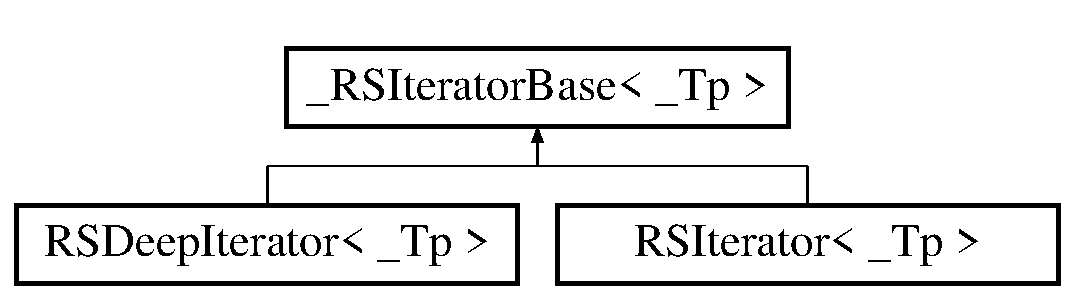
\includegraphics[height=2cm]{class__RSIteratorBase}
\end{center}
\end{figure}
\subsection*{Public Member Functions}
\begin{DoxyCompactItemize}
\item 
{\bfseries \_\-RSIteratorBase} ({\bf RSObj} $\ast$\_\-root)\label{class__RSIteratorBase_af07a7397181c549e9dccda2f1ed00ffa}

\item 
\_\-Tp \& {\bfseries operator$\ast$} ()\label{class__RSIteratorBase_ab2c8eb9b01dca6f47d8229cb797b6ead}

\item 
\_\-Tp $\ast$ {\bfseries operator-\/$>$} ()\label{class__RSIteratorBase_a84c8d55b3d349d466c7b3113e8a5fc18}

\item 
\_\-Tp $\ast$ {\bfseries operator\&} ()\label{class__RSIteratorBase_ae17fe20d0ec34ab179549c172986c740}

\end{DoxyCompactItemize}
\subsection*{Protected Attributes}
\begin{DoxyCompactItemize}
\item 
{\bf RSObj} $\ast$ {\bfseries root}\label{class__RSIteratorBase_af96f1020e4efafc8106508034a64c69a}

\item 
{\bf RSLinkGroup} $\ast$ {\bfseries lg}\label{class__RSIteratorBase_ad54c4d5423dc09135301671c4cbd24b7}

\item 
{\bf RSLink} $\ast$ {\bfseries nxt}\label{class__RSIteratorBase_a1630611fa3ae296aced716c08721c163}

\item 
{\bf RSLink} $\ast$ {\bfseries cur}\label{class__RSIteratorBase_a061cc072cef6ae5f9c849742e59ce700}

\item 
RSType {\bfseries type}\label{class__RSIteratorBase_a4d1df4dc2b03c6d03310ddc85ca3848b}

\end{DoxyCompactItemize}


\subsection{Detailed Description}
\subsubsection*{template$<$class \_\-Tp$>$ class \_\-RSIteratorBase$<$ \_\-Tp $>$}



Definition at line 443 of file RecoUtil.hh.

The documentation for this class was generated from the following file:\begin{DoxyCompactItemize}
\item 
RecoUtil.hh\end{DoxyCompactItemize}

\section{\_\-RSParentIteratorBase$<$ \_\-Tp $>$ Class Template Reference}
\label{class__RSParentIteratorBase}\index{\_\-RSParentIteratorBase@{\_\-RSParentIteratorBase}}
Inheritance diagram for \_\-RSParentIteratorBase$<$ \_\-Tp $>$::\begin{figure}[H]
\begin{center}
\leavevmode
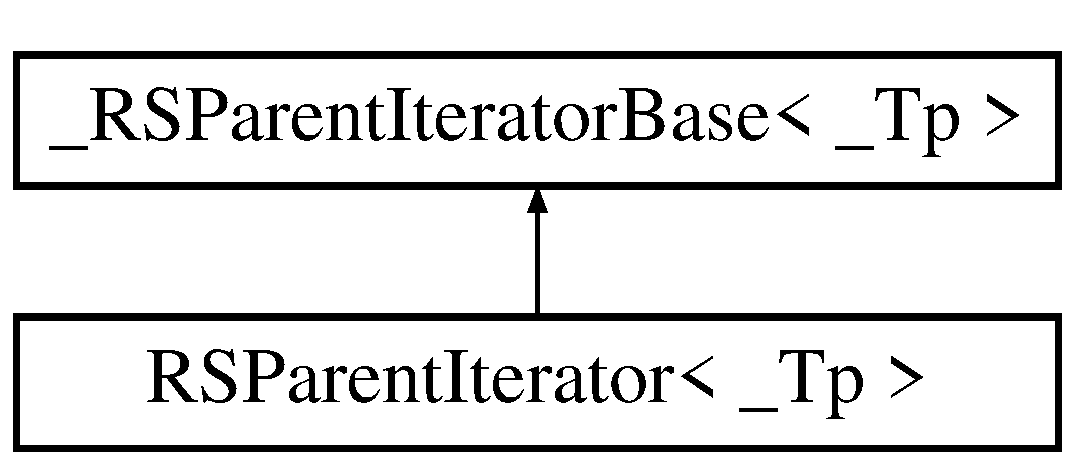
\includegraphics[height=2cm]{class__RSParentIteratorBase}
\end{center}
\end{figure}
\subsection*{Public Member Functions}
\begin{DoxyCompactItemize}
\item 
{\bfseries \_\-RSParentIteratorBase} ({\bf RSObj} $\ast$\_\-root)\label{class__RSParentIteratorBase_a8d94f20fa8429a0d2fb71cff51687af0}

\item 
\_\-Tp \& {\bfseries operator$\ast$} ()\label{class__RSParentIteratorBase_a1c2f4e14e17c6cbde822b8b5443340ff}

\item 
\_\-Tp $\ast$ {\bfseries operator-\/$>$} ()\label{class__RSParentIteratorBase_a6d9145b0e1e626999790890171a58cb4}

\item 
\_\-Tp $\ast$ {\bfseries operator\&} ()\label{class__RSParentIteratorBase_a1a1ca787bb7f8ba776ef0f23792c6485}

\end{DoxyCompactItemize}
\subsection*{Protected Attributes}
\begin{DoxyCompactItemize}
\item 
{\bf RSObj} $\ast$ {\bfseries root}\label{class__RSParentIteratorBase_ac1bd28e65d3b9777a9f16cdee00b7b6e}

\item 
{\bf RSLink} $\ast$ {\bfseries nxt}\label{class__RSParentIteratorBase_a71bbd4437d43e17760315c6178757bbc}

\item 
{\bf RSLink} $\ast$ {\bfseries cur}\label{class__RSParentIteratorBase_a20edc033cc73d5b7c5eb962fc32c78e5}

\item 
RSType {\bfseries type}\label{class__RSParentIteratorBase_a93a2da9e38fa9a9e8a207f131b3b6149}

\end{DoxyCompactItemize}


\subsection{Detailed Description}
\subsubsection*{template$<$class \_\-Tp$>$ class \_\-RSParentIteratorBase$<$ \_\-Tp $>$}



Definition at line 498 of file RecoUtil.hh.

The documentation for this class was generated from the following file:\begin{DoxyCompactItemize}
\item 
RecoUtil.hh\end{DoxyCompactItemize}

\section{HistogrammPT::AxisRange Class Reference}
\label{classHistogrammPT_1_1AxisRange}\index{HistogrammPT::AxisRange@{HistogrammPT::AxisRange}}


Class for axis range.  


{\ttfamily \#include $<$HistogrammPT.h$>$}\subsection*{Public Member Functions}
\begin{DoxyCompactItemize}
\item 
bool {\bfseries set} (const {\bf MinMaxRange}$<$ double $>$ \&\_\-lim, double \_\-step)\label{classHistogrammPT_1_1AxisRange_a2502c6bc3acea4407d8c40f98b8ebbbc}

\item 
unsigned {\bfseries idx} (double val)\label{classHistogrammPT_1_1AxisRange_a9704c7046100d7dde3f6d68e201142f2}

\end{DoxyCompactItemize}
\subsection*{Data Fields}
\begin{DoxyCompactItemize}
\item 
{\bf MinMaxRange}$<$ double $>$ {\bfseries lim}\label{classHistogrammPT_1_1AxisRange_af69eb3b0a5c1444e10943256c2c44484}

\item 
double {\bfseries step}\label{classHistogrammPT_1_1AxisRange_a5ce62b557ca23603c32cc5ad5b5bc52e}

\item 
unsigned {\bfseries n}\label{classHistogrammPT_1_1AxisRange_a145ae4ea2354e5ff0881a69672c23e2a}

\end{DoxyCompactItemize}


\subsection{Detailed Description}
Class for axis range. 

Definition at line 30 of file HistogrammPT.h.

The documentation for this class was generated from the following files:\begin{DoxyCompactItemize}
\item 
HistogrammPT.h\item 
HistogrammPT.cc\end{DoxyCompactItemize}

\section{DeepAnalysis::Cluster Class Reference}
\label{classDeepAnalysis_1_1Cluster}\index{DeepAnalysis::Cluster@{DeepAnalysis::Cluster}}


\doxyref{Cluster}{p.}{classDeepAnalysis_1_1Cluster} is the main object to work with and to keep the main results of the analisys \doxyref{Cluster}{p.}{classDeepAnalysis_1_1Cluster} consists of its properties: like parameters of the inertia tensor, average density, whole volume, a few topological Chisq and pointers to first and last hits in cluster.  


{\ttfamily \#include $<$DeepAnalysis.hh$>$}Inheritance diagram for DeepAnalysis::Cluster::\begin{figure}[H]
\begin{center}
\leavevmode
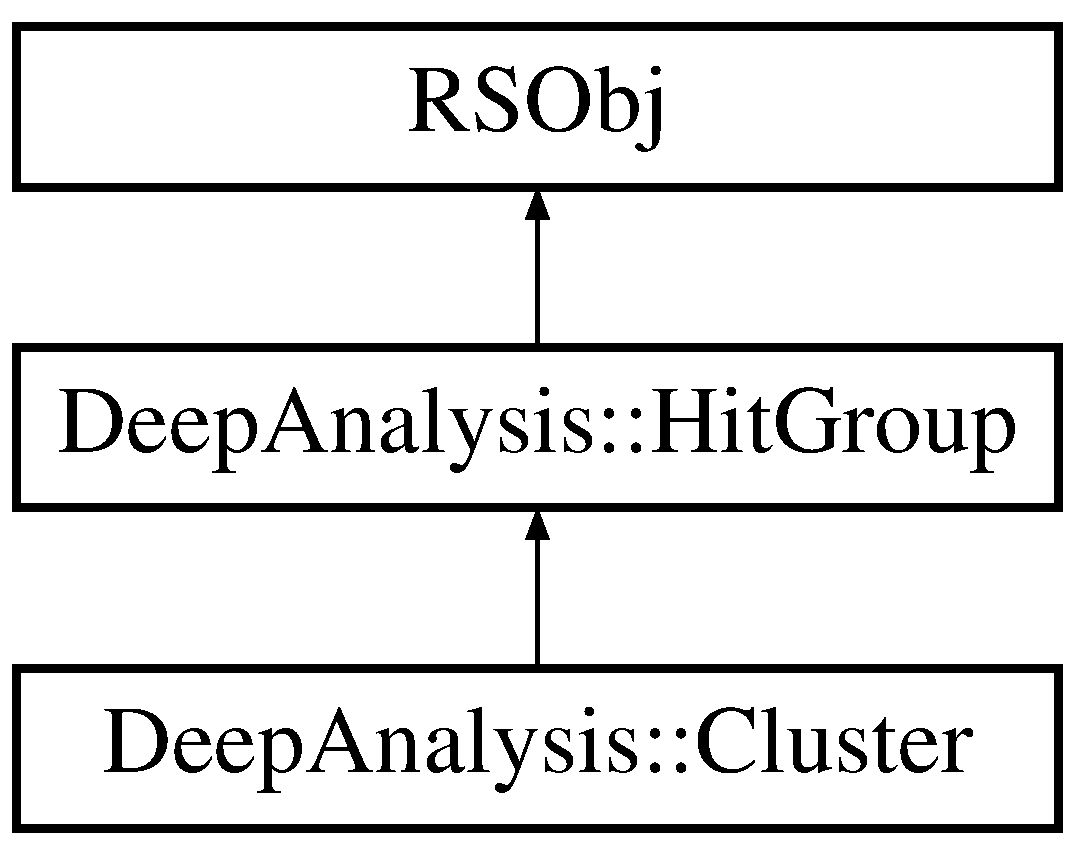
\includegraphics[height=3cm]{classDeepAnalysis_1_1Cluster}
\end{center}
\end{figure}
\subsection*{Public Types}
\begin{DoxyCompactItemize}
\item 
enum \{ \par
{\bf EMPTY}, 
{\bf ONEHIT}, 
{\bf CL2D}, 
{\bf CHAIN}, 
\par
{\bf JOINED}, 
{\bf EXT}
 \}
\begin{DoxyCompactList}\small\item\em An enumeration. \item\end{DoxyCompactList}\end{DoxyCompactItemize}
\subsection*{Public Member Functions}
\begin{DoxyCompactItemize}
\item 
{\bf Cluster} ()\label{classDeepAnalysis_1_1Cluster_ab9a273e3a8e188deaf3edc3d9ec20ab0}

\begin{DoxyCompactList}\small\item\em Constructor. \item\end{DoxyCompactList}\item 
void {\bf calc\_\-color} ({\bf DeepAnalysis} \&rs)\label{classDeepAnalysis_1_1Cluster_ae51c00039fbcf1b6308a3a596a371fd2}

\begin{DoxyCompactList}\small\item\em Set the cluster color depending on the hit and cluster type and colors. \item\end{DoxyCompactList}\item 
void {\bf inertia\_\-3d} (float $\ast$wr)\label{classDeepAnalysis_1_1Cluster_a53d3ab2e062c3c05de19a5bb977f0b91}

\begin{DoxyCompactList}\small\item\em Calculate cluster tensor of inertia and its principal axes. \item\end{DoxyCompactList}\item 
void {\bf calc\_\-prop} ({\bf DeepAnalysis} \&rs, bool for\_\-em=false)\label{classDeepAnalysis_1_1Cluster_a1b6a9b571ebf340ddba682a51be515e4}

\begin{DoxyCompactList}\small\item\em Calculate properties of \doxyref{Cluster}{p.}{classDeepAnalysis_1_1Cluster}. \item\end{DoxyCompactList}\item 
void {\bf finalize} ({\bf DeepAnalysis} \&rs)\label{classDeepAnalysis_1_1Cluster_ab88af1f7e158cfa3ffd262ad28fd5c3d}

\begin{DoxyCompactList}\small\item\em Finalize: mainly works with the rest of the hits that do not belongs to any cluster and also recolored some of the clusters. \item\end{DoxyCompactList}\item 
void {\bf rotate\_\-point} (Point3D \&point)
\begin{DoxyCompactList}\small\item\em Rotate 3D point. \item\end{DoxyCompactList}\item 
void {\bf print} ()\label{classDeepAnalysis_1_1Cluster_ace18b07f58322eac1dbc7a234b377e31}

\begin{DoxyCompactList}\small\item\em Print out info. \item\end{DoxyCompactList}\item 
void {\bf line} (const Point3D \&p0, const Point3D \&p1, unsigned {\bf type}, unsigned size, unsigned color)\label{classDeepAnalysis_1_1Cluster_a89f061c2bc38c88fbf842f3c694f01db}

\begin{DoxyCompactList}\small\item\em Draw line between 2 points. \item\end{DoxyCompactList}\item 
void {\bf draw\_\-star} (unsigned {\bf type}, unsigned color)\label{classDeepAnalysis_1_1Cluster_ac516666e7c03195b1e1fa11787552494}

\begin{DoxyCompactList}\small\item\em Draw star. \item\end{DoxyCompactList}\item 
void {\bf draw\_\-tree} (unsigned {\bf type}, unsigned color)
\begin{DoxyCompactList}\small\item\em Draw tree. \item\end{DoxyCompactList}\item 
void {\bf draw\_\-ellipse} (unsigned {\bf type}, unsigned color)\label{classDeepAnalysis_1_1Cluster_a9d7f5c176df6785e8dcf8f1d3ead0eea}

\begin{DoxyCompactList}\small\item\em Draw ellipsoid. \item\end{DoxyCompactList}\end{DoxyCompactItemize}
\subsection*{Data Fields}
\begin{DoxyCompactItemize}
\item 
enum DeepAnalysis::Cluster:: \{ ... \}  {\bf type}\label{classDeepAnalysis_1_1Cluster_ad204dc8ea429d6bafbedc19aab8299a0}

\begin{DoxyCompactList}\small\item\em An enumeration. \item\end{DoxyCompactList}\item 
Sphere3D {\bf sp2d}\label{classDeepAnalysis_1_1Cluster_a4a293fe7d9a0d78506c4d13fbdb0c13f}

\begin{DoxyCompactList}\small\item\em temporary variable, for use in 2D clustering \item\end{DoxyCompactList}\item 
double {\bf e2d}\label{classDeepAnalysis_1_1Cluster_a4cec96aed3a9af9653b6412406ae95be}

\begin{DoxyCompactList}\small\item\em temporary variable, for use in 2D clustering \item\end{DoxyCompactList}\item 
{\bf KIND} {\bf col}\label{classDeepAnalysis_1_1Cluster_adeb3b57d6dd388878ca239508beec600}

\begin{DoxyCompactList}\small\item\em type (M\_\-cl\_\-col) \item\end{DoxyCompactList}\item 
Vector3D {\bf clusterAxisVector}\label{classDeepAnalysis_1_1Cluster_a3425bd5baead7b66119095fd75067b7f}

\begin{DoxyCompactList}\small\item\em main principal axis (Cx\_\-clust) \item\end{DoxyCompactList}\item 
double {\bf clusterRadius}\label{classDeepAnalysis_1_1Cluster_ad4975a52e8c168074ce7493c57271420}

\begin{DoxyCompactList}\small\item\em radius vector length (R\_\-clust) \item\end{DoxyCompactList}\item 
double {\bf clusterLongestRadius}\label{classDeepAnalysis_1_1Cluster_a6fb307299011bdd227c81bd429672206}

\begin{DoxyCompactList}\small\item\em longest radius (r1\_\-clust) \item\end{DoxyCompactList}\item 
double {\bf forwRadius}\label{classDeepAnalysis_1_1Cluster_a36fc7d171877ef8084e7ab3f944d4018}

\begin{DoxyCompactList}\small\item\em forward radius \item\end{DoxyCompactList}\item 
double {\bf backwRadius}\label{classDeepAnalysis_1_1Cluster_ac7ae47244c3cbd8c2b6e63412cb3fe2f}

\begin{DoxyCompactList}\small\item\em backward radius \item\end{DoxyCompactList}\item 
double {\bf r2}\label{classDeepAnalysis_1_1Cluster_a4e918af2cb90f1a9b91cb8d94d2180aa}

\begin{DoxyCompactList}\small\item\em short one \item\end{DoxyCompactList}\item 
double {\bf r3}\label{classDeepAnalysis_1_1Cluster_a2d16c60415ab31b3a90d37abb4252de9}

\begin{DoxyCompactList}\small\item\em short two \item\end{DoxyCompactList}\item 
double {\bf ecc}\label{classDeepAnalysis_1_1Cluster_a980eb35cf5fa3c1fda5857ad911f37ec}

\begin{DoxyCompactList}\small\item\em eccentricity (ecc\_\-clust) \item\end{DoxyCompactList}\item 
double {\bf ellipAverageRadius}\label{classDeepAnalysis_1_1Cluster_a3801c3f27c4a245951c99bcacaa74b68}

\begin{DoxyCompactList}\small\item\em elipsoid average radius \item\end{DoxyCompactList}\item 
double {\bf volume}\label{classDeepAnalysis_1_1Cluster_aac8bbd1695898f7c5f0367d33301bb8c}

\begin{DoxyCompactList}\small\item\em elipsoid volume \item\end{DoxyCompactList}\item 
double {\bf density}\label{classDeepAnalysis_1_1Cluster_aada07d33993528136a3815783a006db3}

\begin{DoxyCompactList}\small\item\em cluster density \item\end{DoxyCompactList}\item 
double {\bf chi} [3]\label{classDeepAnalysis_1_1Cluster_a4bdb105189350d277eb669bd1be45f66}

\begin{DoxyCompactList}\small\item\em Chisquare W -\/ quadratic, W linear, W=1 -\/ pure spatial. \item\end{DoxyCompactList}\item 
{\bf Hit} $\ast$ {\bf begn}\label{classDeepAnalysis_1_1Cluster_a7c1a3b2beb89d28a926e975a3889aacf}

\begin{DoxyCompactList}\small\item\em address of first cluster point (L\_\-cl\_\-begn) \item\end{DoxyCompactList}\item 
{\bf Hit} $\ast$ {\bf last}\label{classDeepAnalysis_1_1Cluster_a6b72c48bea2c4fe6cd6f5d6b80cc45c1}

\begin{DoxyCompactList}\small\item\em address of last cluster point (L\_\-cl\_\-last) \item\end{DoxyCompactList}\item 
double {\bfseries v1} [3]\label{classDeepAnalysis_1_1Cluster_a03fd541ee1458241de240db5432b36f6}

\item 
double {\bfseries v2} [3]\label{classDeepAnalysis_1_1Cluster_aeec5e4fedcbf07aa8fe10dc451ed7941}

\item 
double {\bf v3} [3]\label{classDeepAnalysis_1_1Cluster_a8b748f394bfee834ad0441d107b2accd}

\begin{DoxyCompactList}\small\item\em elipsoid axis \item\end{DoxyCompactList}\end{DoxyCompactItemize}
\subsection*{Static Public Attributes}
\begin{DoxyCompactItemize}
\item 
static const unsigned {\bf RS\_\-TYPE} = 6\label{classDeepAnalysis_1_1Cluster_aa72122f9aef00ce8f424dc6484449937}

\begin{DoxyCompactList}\small\item\em type of \doxyref{RS}{p.}{classRS} object \item\end{DoxyCompactList}\end{DoxyCompactItemize}


\subsection{Detailed Description}
\doxyref{Cluster}{p.}{classDeepAnalysis_1_1Cluster} is the main object to work with and to keep the main results of the analisys \doxyref{Cluster}{p.}{classDeepAnalysis_1_1Cluster} consists of its properties: like parameters of the inertia tensor, average density, whole volume, a few topological Chisq and pointers to first and last hits in cluster. 

Definition at line 325 of file DeepAnalysis.hh.

\subsection{Member Enumeration Documentation}
\subsubsection[{"@0}]{\setlength{\rightskip}{0pt plus 5cm}anonymous enum}\label{classDeepAnalysis_1_1Cluster_af5293b0f3ebc5caf2273b669e5645077}


An enumeration. \begin{Desc}
\item[Enumerator: ]\par
\begin{description}
\index{EMPTY@{EMPTY}!DeepAnalysis::Cluster@{DeepAnalysis::Cluster}}\index{DeepAnalysis::Cluster@{DeepAnalysis::Cluster}!EMPTY@{EMPTY}}\item[{\em 
EMPTY\label{classDeepAnalysis_1_1Cluster_af5293b0f3ebc5caf2273b669e5645077a72a88701d4eca87d7a4d10718ec58713}
}]empty (no hit) \index{ONEHIT@{ONEHIT}!DeepAnalysis::Cluster@{DeepAnalysis::Cluster}}\index{DeepAnalysis::Cluster@{DeepAnalysis::Cluster}!ONEHIT@{ONEHIT}}\item[{\em 
ONEHIT\label{classDeepAnalysis_1_1Cluster_af5293b0f3ebc5caf2273b669e5645077ab47d5f340993268b096bdcad05af9bb1}
}]contains one hit \index{CL2D@{CL2D}!DeepAnalysis::Cluster@{DeepAnalysis::Cluster}}\index{DeepAnalysis::Cluster@{DeepAnalysis::Cluster}!CL2D@{CL2D}}\item[{\em 
CL2D\label{classDeepAnalysis_1_1Cluster_af5293b0f3ebc5caf2273b669e5645077adf70ce9e9700cddc5edd761a4fef0464}
}]2D cluster \index{CHAIN@{CHAIN}!DeepAnalysis::Cluster@{DeepAnalysis::Cluster}}\index{DeepAnalysis::Cluster@{DeepAnalysis::Cluster}!CHAIN@{CHAIN}}\item[{\em 
CHAIN\label{classDeepAnalysis_1_1Cluster_af5293b0f3ebc5caf2273b669e5645077a1e5debab6e368782edb56427399cb41b}
}]chain \index{JOINED@{JOINED}!DeepAnalysis::Cluster@{DeepAnalysis::Cluster}}\index{DeepAnalysis::Cluster@{DeepAnalysis::Cluster}!JOINED@{JOINED}}\item[{\em 
JOINED\label{classDeepAnalysis_1_1Cluster_af5293b0f3ebc5caf2273b669e5645077a81c25157b39debd5e46d8f2cc87805cb}
}]joined \index{EXT@{EXT}!DeepAnalysis::Cluster@{DeepAnalysis::Cluster}}\index{DeepAnalysis::Cluster@{DeepAnalysis::Cluster}!EXT@{EXT}}\item[{\em 
EXT\label{classDeepAnalysis_1_1Cluster_af5293b0f3ebc5caf2273b669e5645077a1f478e59def62f3981ba8ae6c1ce1da7}
}]external \end{description}
\end{Desc}



Definition at line 330 of file DeepAnalysis.hh.

\subsection{Member Function Documentation}
\index{DeepAnalysis::Cluster@{DeepAnalysis::Cluster}!draw\_\-tree@{draw\_\-tree}}
\index{draw\_\-tree@{draw\_\-tree}!DeepAnalysis::Cluster@{DeepAnalysis::Cluster}}
\subsubsection[{draw\_\-tree}]{\setlength{\rightskip}{0pt plus 5cm}void DeepAnalysis::Cluster::draw\_\-tree (unsigned {\em type}, \/  unsigned {\em color})\hspace{0.3cm}{\ttfamily  [inline]}}\label{classDeepAnalysis_1_1Cluster_a869d6edc0f3b1bffb5e27804662531c4}


Draw tree. .. 

Definition at line 678 of file DeepAnalysis.hh.

References begn, DeepAnalysis::Hit::cartesianPoint, and line().\index{DeepAnalysis::Cluster@{DeepAnalysis::Cluster}!rotate\_\-point@{rotate\_\-point}}
\index{rotate\_\-point@{rotate\_\-point}!DeepAnalysis::Cluster@{DeepAnalysis::Cluster}}
\subsubsection[{rotate\_\-point}]{\setlength{\rightskip}{0pt plus 5cm}void DeepAnalysis::Cluster::rotate\_\-point (Point3D \& {\em point})\hspace{0.3cm}{\ttfamily  [inline]}}\label{classDeepAnalysis_1_1Cluster_aa639336101fc5d3a49fa32ce35fc69c2}


Rotate 3D point. 
\begin{DoxyParams}{Parameters}
\item[{\em point}]3D point where to rotate \end{DoxyParams}


Definition at line 633 of file DeepAnalysis.hh.

References DeepAnalysis::HitGroup::centerOfGravity, and v3.

Referenced by draw\_\-ellipse().

The documentation for this class was generated from the following file:\begin{DoxyCompactItemize}
\item 
DeepAnalysis.hh\end{DoxyCompactItemize}

\section{DeepAnalysis Class Reference}
\label{classDeepAnalysis}\index{DeepAnalysis@{DeepAnalysis}}


\doxyref{Cluster}{p.}{classDeepAnalysis_1_1Cluster} finding and analysis.  


{\ttfamily \#include $<$DeepAnalysis.hh$>$}Inheritance diagram for DeepAnalysis::\begin{figure}[H]
\begin{center}
\leavevmode
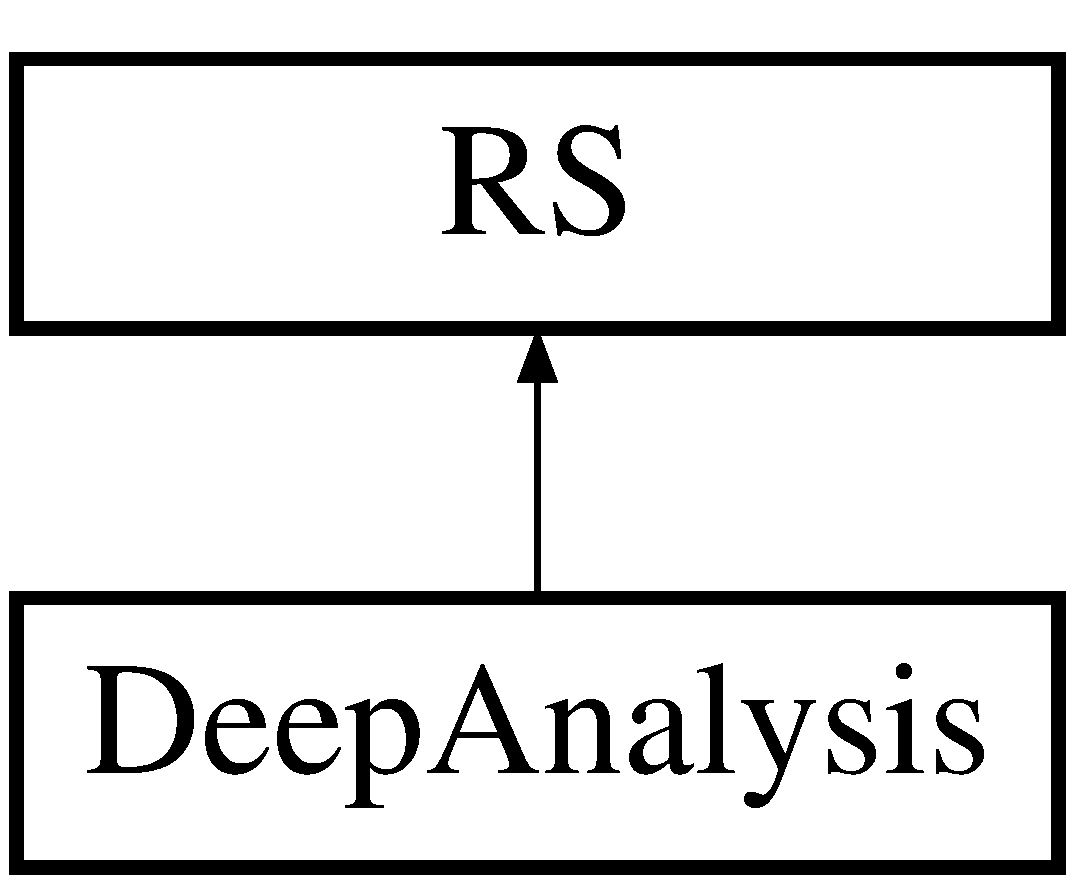
\includegraphics[height=2cm]{classDeepAnalysis}
\end{center}
\end{figure}
\subsection*{Data Structures}
\begin{DoxyCompactItemize}
\item 
class {\bf Cluster}
\begin{DoxyCompactList}\small\item\em \doxyref{Cluster}{p.}{classDeepAnalysis_1_1Cluster} is the main object to work with and to keep the main results of the analisys \doxyref{Cluster}{p.}{classDeepAnalysis_1_1Cluster} consists of its properties: like parameters of the inertia tensor, average density, whole volume, a few topological Chisq and pointers to first and last hits in cluster. \item\end{DoxyCompactList}\item 
class {\bf Detector}
\begin{DoxyCompactList}\small\item\em Class for detector and algorithm parameters. \item\end{DoxyCompactList}\item 
class {\bf Group}
\begin{DoxyCompactList}\small\item\em Class for general multipurpose grouping. \item\end{DoxyCompactList}\item 
class {\bf Hit}
\begin{DoxyCompactList}\small\item\em Class for hit: consists of:. \item\end{DoxyCompactList}\item 
class {\bf HitGroup}
\begin{DoxyCompactList}\small\item\em This class is not a cluster, but this is as it said in name -\/-\/ \doxyref{Group}{p.}{classDeepAnalysis_1_1Group} of Hits, that has a boundaries in 3-\/D cartesian coordinate system and spherical coordinate system, center of gravity and whole energy. \item\end{DoxyCompactList}\item 
class {\bf JoinGroup}
\begin{DoxyCompactList}\small\item\em Class for joining groups (juts a working intermediate class) (for \doxyref{cluster\_\-join}{p.}{classDeepAnalysis_a11f0ad635e5acf4b82c36170b9db6293} method). \item\end{DoxyCompactList}\item 
class {\bf KindGroup}
\begin{DoxyCompactList}\small\item\em This class has a represents of RGB types of Groups. \item\end{DoxyCompactList}\item 
class {\bf NeutGroup}
\begin{DoxyCompactList}\small\item\em Neutrons group (specific for technical reasons). \item\end{DoxyCompactList}\item 
class {\bf SpecialHist2D}
\begin{DoxyCompactList}\small\item\em Special 2D histograms. \item\end{DoxyCompactList}\end{DoxyCompactItemize}
\subsection*{Public Types}
\begin{DoxyCompactItemize}
\item 
enum {\bf KIND} \{ \par
{\bf EM} = 0, 
{\bf TRK}, 
{\bf HAD}, 
{\bf KIND\_\-COUNT}, 
\par
{\bf NEUTR}
 \}
\begin{DoxyCompactList}\small\item\em An enumeration -\/-\/ colors for RGB scheme for hit spectrum RED is most dense hit(calorimeter cell) BLUE is intermediate GREEN is MIP-\/like, or around the MIP density. \item\end{DoxyCompactList}\end{DoxyCompactItemize}
\subsection*{Public Member Functions}
\begin{DoxyCompactItemize}
\item 
{\bf DeepAnalysis} ()\label{classDeepAnalysis_a922be045364409dca5f7fdc517dceea7}

\begin{DoxyCompactList}\small\item\em Constructor. \item\end{DoxyCompactList}\item 
void {\bf cluster\_\-from\_\-singles} ({\bf KindGroup} \&gr, bool mark\_\-neutrons)\label{classDeepAnalysis_a3272cc7e90359df6241e0ef5d3493d09}

\begin{DoxyCompactList}\small\item\em Create clusters from single hits. \item\end{DoxyCompactList}\item 
void {\bf cluster\_\-finder\_\-2d\_\-split} ({\bf Hit} \&hit, unsigned InClust\_\-count, {\bf Cluster} $\ast$$\ast$InClust)\label{classDeepAnalysis_a51aa039e800972d2eb4bb9dce5a99783}

\begin{DoxyCompactList}\small\item\em Distribute hits at the spherical shell onto found 2D cluster seeds. \item\end{DoxyCompactList}\item 
void {\bf cluster\_\-finder\_\-2d} ({\bf HitGroup} \&hitGroup, {\bf Group} \&ring)\label{classDeepAnalysis_abf4d67264d95678b7fd012d1e053c551}

\begin{DoxyCompactList}\small\item\em 2D clustering procedure to find clusters by histogramming technique at the one spherical shell in Theta-\/Phi. \item\end{DoxyCompactList}\item 
void {\bf cluster\_\-finder\_\-3d} ({\bf KindGroup} \&gr, bool mark\_\-neutrons)
\begin{DoxyCompactList}\small\item\em Find 3D clusters. \item\end{DoxyCompactList}\item 
void {\bf join\_\-group} ({\bf Cluster} $\ast$cl, {\bf JoinGroup} $\ast$jg)\label{classDeepAnalysis_ac71417b351b1863345d8dc5fe03e1107}

\begin{DoxyCompactList}\small\item\em Technical function used in cluster\_\-join. \item\end{DoxyCompactList}\item 
void {\bf make\_\-join\_\-group} ({\bf Cluster} $\ast$cl0, {\bf Cluster} $\ast$cl1, {\bf Cluster} $\ast$cl2=0)\label{classDeepAnalysis_a86fa610ab5bc688a31ac2637df3e17b8}

\begin{DoxyCompactList}\small\item\em Technical function used in cluster\_\-join. \item\end{DoxyCompactList}\item 
void {\bf cluster\_\-join} (bool for\_\-em)\label{classDeepAnalysis_a11f0ad635e5acf4b82c36170b9db6293}

\begin{DoxyCompactList}\small\item\em Join clusters together. \item\end{DoxyCompactList}\item 
void {\bf em\_\-shower\_\-find} ()\label{classDeepAnalysis_a430c22c153af3cc4213d8f4278000c3a}

\begin{DoxyCompactList}\small\item\em Find electromagnetic shower: it collects additional (not RED) hits around the EM cluster core. \item\end{DoxyCompactList}\item 
void {\bf reassignment\_\-small\_\-clusters} ({\bf KIND} k)\label{classDeepAnalysis_a6248d82766ae25095c0c02b8ba6d2814}

\begin{DoxyCompactList}\small\item\em Reassign small clusters. \item\end{DoxyCompactList}\item 
void {\bf low\_\-e\_\-clean} ()\label{classDeepAnalysis_a3c0d64094110d97819ea2910d9ae5c8e}

\begin{DoxyCompactList}\small\item\em Clean low energy clusters. \item\end{DoxyCompactList}\item 
{\bf Hit} $\ast$ {\bf add\_\-hit} (double \_\-x, double \_\-y, double \_\-z, double \_\-am, double \_\-ampl\_\-mip, double \_\-thr, unsigned \_\-lay, {\bf KIND} type, int \_\-addr)\label{classDeepAnalysis_ace5c5cc371d13a3a3e4c4bb7c1e6c7a4}

\begin{DoxyCompactList}\small\item\em Create \doxyref{Hit}{p.}{classDeepAnalysis_1_1Hit} object. \item\end{DoxyCompactList}\item 
void {\bf draw} ()\label{classDeepAnalysis_a3296261a9ec689302d1d0105f0b70a6b}

\begin{DoxyCompactList}\small\item\em Draw ?? \item\end{DoxyCompactList}\item 
void {\bf draw\_\-to\_\-layer} (unsigned layer)\label{classDeepAnalysis_af86fccd30742311ff86392d997e6ad36}

\begin{DoxyCompactList}\small\item\em Draw ?? \item\end{DoxyCompactList}\item 
void {\bf color\_\-clusters\_\-stat} ({\bf KIND} k, unsigned \&ncl, unsigned \&n\_\-sum, double \&e\_\-sum)
\begin{DoxyCompactList}\small\item\em Calculate cluster statistics. \item\end{DoxyCompactList}\item 
void {\bf color\_\-clusters\_\-print\_\-stat} ({\bf KIND} k)
\begin{DoxyCompactList}\small\item\em Print clusters statistics. \item\end{DoxyCompactList}\item 
void {\bf result\_\-check} ()\label{classDeepAnalysis_a580d9000ca7ac7a8144ade2abf20f721}

\begin{DoxyCompactList}\small\item\em Check result. \item\end{DoxyCompactList}\item 
void {\bf event\_\-move} ()\label{classDeepAnalysis_adf15194da18059e69c5bd736bc33b308}

\begin{DoxyCompactList}\small\item\em Move event from a pole to equator of spherical coordinate system. \item\end{DoxyCompactList}\item 
void {\bf event\_\-move\_\-back} ()\label{classDeepAnalysis_ac7963f23fe529d8e0074df287ce961f8}

\begin{DoxyCompactList}\small\item\em Move back event to the pole of Sp\_\-CS. \item\end{DoxyCompactList}\item 
void {\bf reconstruction} ()
\begin{DoxyCompactList}\small\item\em Main routine to split event into four different types of clusters: EM -\/ electromagnetic piece of hadronic shower TRK -\/ tracks in hadronic shower HAD -\/ a few tracks in hadronic shower that cannot be splitted into individual tracks. \item\end{DoxyCompactList}\end{DoxyCompactItemize}
\subsection*{Data Fields}
\begin{DoxyCompactItemize}
\item 
{\bf Detector} {\bfseries detector}\label{classDeepAnalysis_ae8df2c2ff1e0c18d7a10f54ba1ce2f2b}

\item 
{\bf HitGroup} $\ast$ {\bf all\_\-hits}
\begin{DoxyCompactList}\small\item\em All main pointer to structures. \item\end{DoxyCompactList}\item 
{\bf Group} $\ast$ {\bf clusters}\label{classDeepAnalysis_a2ebb35e99adf044cf85cc88fa8d3fa0d}

\begin{DoxyCompactList}\small\item\em clusters \item\end{DoxyCompactList}\item 
{\bf Group} $\ast$ {\bf joingroups}\label{classDeepAnalysis_a3d81237d4f1f894876149f096059217b}

\begin{DoxyCompactList}\small\item\em joined groups \item\end{DoxyCompactList}\item 
{\bf KindGroup} $\ast$ {\bf kind} [KIND\_\-COUNT]\label{classDeepAnalysis_a63269ac67462b5e1a5891a6fcc36e831}

\begin{DoxyCompactList}\small\item\em hit type \item\end{DoxyCompactList}\item 
{\bf NeutGroup} $\ast$ {\bf neutrons}\label{classDeepAnalysis_a0bccfdab6b95f7d359995a82da828ebd}

\begin{DoxyCompactList}\small\item\em neutrons group \item\end{DoxyCompactList}\item 
unsigned {\bf all\_\-hits\_\-count}\label{classDeepAnalysis_afa56405784e372bdf9c7f11fc59f1bf9}

\begin{DoxyCompactList}\small\item\em counter for all hits \item\end{DoxyCompactList}\end{DoxyCompactItemize}


\subsection{Detailed Description}
\doxyref{Cluster}{p.}{classDeepAnalysis_1_1Cluster} finding and analysis. Hadronic shower analysis using hit density, shower topology and cluster shapes to find shower component of different physical origin, such as pure tracks, electromagnetic cascades inside hadronic shower; and hits that produced by neutrons.

\begin{DoxyAuthor}{Author}
V.L. Morgunov 
\end{DoxyAuthor}
\begin{DoxyDate}{Date}
18 September 2007 
\end{DoxyDate}


Definition at line 52 of file DeepAnalysis.hh.

\subsection{Member Enumeration Documentation}
\index{DeepAnalysis@{DeepAnalysis}!KIND@{KIND}}
\index{KIND@{KIND}!DeepAnalysis@{DeepAnalysis}}
\subsubsection[{KIND}]{\setlength{\rightskip}{0pt plus 5cm}enum {\bf DeepAnalysis::KIND}}\label{classDeepAnalysis_a8e37d65f57d59e268a839b039848815c}


An enumeration -\/-\/ colors for RGB scheme for hit spectrum RED is most dense hit(calorimeter cell) BLUE is intermediate GREEN is MIP-\/like, or around the MIP density. \begin{Desc}
\item[Enumerator: ]\par
\begin{description}
\index{EM@{EM}!DeepAnalysis@{DeepAnalysis}}\index{DeepAnalysis@{DeepAnalysis}!EM@{EM}}\item[{\em 
EM\label{classDeepAnalysis_a8e37d65f57d59e268a839b039848815ca3993fe069642f9ef25af6471a711ba7a}
}]former 2 color red \index{TRK@{TRK}!DeepAnalysis@{DeepAnalysis}}\index{DeepAnalysis@{DeepAnalysis}!TRK@{TRK}}\item[{\em 
TRK\label{classDeepAnalysis_a8e37d65f57d59e268a839b039848815ca15b5219f26836651924a14051eeacee6}
}]former 3 color green \index{HAD@{HAD}!DeepAnalysis@{DeepAnalysis}}\index{DeepAnalysis@{DeepAnalysis}!HAD@{HAD}}\item[{\em 
HAD\label{classDeepAnalysis_a8e37d65f57d59e268a839b039848815ca9f39fc8015a438a8f8140a4519d46810}
}]former 4 color blue \index{KIND\_\-COUNT@{KIND\_\-COUNT}!DeepAnalysis@{DeepAnalysis}}\index{DeepAnalysis@{DeepAnalysis}!KIND\_\-COUNT@{KIND\_\-COUNT}}\item[{\em 
KIND\_\-COUNT\label{classDeepAnalysis_a8e37d65f57d59e268a839b039848815ca0edf8eebee148f30a1dac100dcb70d96}
}]counter for kinds (types) \index{NEUTR@{NEUTR}!DeepAnalysis@{DeepAnalysis}}\index{DeepAnalysis@{DeepAnalysis}!NEUTR@{NEUTR}}\item[{\em 
NEUTR\label{classDeepAnalysis_a8e37d65f57d59e268a839b039848815ca460d128073038dbfb0e1d21a1cca3e61}
}]after count, since it is not \doxyref{KindGroup}{p.}{classDeepAnalysis_1_1KindGroup}. \end{description}
\end{Desc}



Definition at line 159 of file DeepAnalysis.hh.

\subsection{Member Function Documentation}
\index{DeepAnalysis@{DeepAnalysis}!cluster\_\-finder\_\-3d@{cluster\_\-finder\_\-3d}}
\index{cluster\_\-finder\_\-3d@{cluster\_\-finder\_\-3d}!DeepAnalysis@{DeepAnalysis}}
\subsubsection[{cluster\_\-finder\_\-3d}]{\setlength{\rightskip}{0pt plus 5cm}void DeepAnalysis::cluster\_\-finder\_\-3d ({\bf KindGroup} \& {\em gr}, \/  bool {\em mark\_\-neutrons})\hspace{0.3cm}{\ttfamily  [inline]}}\label{classDeepAnalysis_a0f5264f0bbbab0caf1069c8faafc3d25}


Find 3D clusters. Method is: to create spherilal shells in the event volume, make 2D clustering at each shell, then connect near by 2D clusters into 3D trees. 

!!!!!!!!!!!!!!!!!!!!!!!!!!!!!!!!!!!!!!!!!!!!!!!!!!!!!!!!!!!!!!!!!

!!!!!!!!!!!!!!!!!!!!!!!!!!!!!!!!!!!!!!!!!!!!!!!!!!!!!!!!!!!!!!!!! 

Definition at line 1003 of file DeepAnalysis.hh.

References DeepAnalysis::Cluster::calc\_\-prop(), DeepAnalysis::HitGroup::calc\_\-stat(), DeepAnalysis::Cluster::CHAIN, cluster\_\-finder\_\-2d(), cluster\_\-from\_\-singles(), clusters, DeepAnalysis::Cluster::EMPTY, DeepAnalysis::Detector::ext\_\-cell\_\-size, HAD, DeepAnalysis::Detector::join\_\-factor, kind, DeepAnalysis::HitGroup::layer\_\-g, Range$<$ \_\-T $>$::max, Range$<$ \_\-T $>$::min, DeepAnalysis::Cluster::ONEHIT, DeepAnalysis::HitGroup::radius\_\-g, DeepAnalysis::Detector::sampling, TRK, and DeepAnalysis::Cluster::type.

Referenced by reconstruction().\index{DeepAnalysis@{DeepAnalysis}!color\_\-clusters\_\-print\_\-stat@{color\_\-clusters\_\-print\_\-stat}}
\index{color\_\-clusters\_\-print\_\-stat@{color\_\-clusters\_\-print\_\-stat}!DeepAnalysis@{DeepAnalysis}}
\subsubsection[{color\_\-clusters\_\-print\_\-stat}]{\setlength{\rightskip}{0pt plus 5cm}void DeepAnalysis::color\_\-clusters\_\-print\_\-stat ({\bf KIND} {\em k})\hspace{0.3cm}{\ttfamily  [inline]}}\label{classDeepAnalysis_afdc891004ebb437b7058ed0cc9068164}


Print clusters statistics. 
\begin{DoxyParams}{Parameters}
\item[{\em k}]kind of cluster \end{DoxyParams}


Definition at line 1514 of file DeepAnalysis.hh.

References color\_\-clusters\_\-stat().\index{DeepAnalysis@{DeepAnalysis}!color\_\-clusters\_\-stat@{color\_\-clusters\_\-stat}}
\index{color\_\-clusters\_\-stat@{color\_\-clusters\_\-stat}!DeepAnalysis@{DeepAnalysis}}
\subsubsection[{color\_\-clusters\_\-stat}]{\setlength{\rightskip}{0pt plus 5cm}void DeepAnalysis::color\_\-clusters\_\-stat ({\bf KIND} {\em k}, \/  unsigned \& {\em ncl}, \/  unsigned \& {\em n\_\-sum}, \/  double \& {\em e\_\-sum})\hspace{0.3cm}{\ttfamily  [inline]}}\label{classDeepAnalysis_a6c35bfd21af8c49247ac819935b744a5}


Calculate cluster statistics. 
\begin{DoxyParams}{Parameters}
\item[{\em k}]type of cluster \item[{\em ncl}]number of clusters \item[{\em n\_\-sum}]total number of hits \item[{\em e\_\-sum}]total energy sum \end{DoxyParams}


Definition at line 1499 of file DeepAnalysis.hh.

References clusters.

Referenced by color\_\-clusters\_\-print\_\-stat(), and CALICE::DeepAnalysisProcessor::processEvent().\index{DeepAnalysis@{DeepAnalysis}!reconstruction@{reconstruction}}
\index{reconstruction@{reconstruction}!DeepAnalysis@{DeepAnalysis}}
\subsubsection[{reconstruction}]{\setlength{\rightskip}{0pt plus 5cm}void DeepAnalysis::reconstruction ()\hspace{0.3cm}{\ttfamily  [inline]}}\label{classDeepAnalysis_a44b9f2a02510918b2c5909045a8beb19}


Main routine to split event into four different types of clusters: EM -\/ electromagnetic piece of hadronic shower TRK -\/ tracks in hadronic shower HAD -\/ a few tracks in hadronic shower that cannot be splitted into individual tracks. NEUT -\/ neutron component of hadronic shower 

Definition at line 1599 of file DeepAnalysis.hh.

References all\_\-hits, DeepAnalysis::HitGroup::calc\_\-stat(), cluster\_\-finder\_\-3d(), cluster\_\-join(), clusters, EM, em\_\-shower\_\-find(), event\_\-move(), event\_\-move\_\-back(), HAD, DeepAnalysis::Detector::init(), kind, Range$<$ \_\-T $>$::min, DeepAnalysis::HitGroup::radius\_\-g, reassignment\_\-small\_\-clusters(), and TRK.

Referenced by CALICE::DeepAnalysisProcessor::processEvent().

\subsection{Field Documentation}
\index{DeepAnalysis@{DeepAnalysis}!all\_\-hits@{all\_\-hits}}
\index{all\_\-hits@{all\_\-hits}!DeepAnalysis@{DeepAnalysis}}
\subsubsection[{all\_\-hits}]{\setlength{\rightskip}{0pt plus 5cm}{\bf HitGroup}$\ast$ {\bf DeepAnalysis::all\_\-hits}}\label{classDeepAnalysis_a1cc6f5295b6a6ea5f74abc9d7b2f4236}


All main pointer to structures. hit group 

Definition at line 772 of file DeepAnalysis.hh.

Referenced by add\_\-hit(), DeepAnalysis(), em\_\-shower\_\-find(), event\_\-move(), event\_\-move\_\-back(), reconstruction(), and result\_\-check().

The documentation for this class was generated from the following file:\begin{DoxyCompactItemize}
\item 
DeepAnalysis.hh\end{DoxyCompactItemize}

\section{CALICE::DeepAnalysisProcessor Class Reference}
\label{classCALICE_1_1DeepAnalysisProcessor}\index{CALICE::DeepAnalysisProcessor@{CALICE::DeepAnalysisProcessor}}


Processor for the deep analysis according to the algorithm developed by Vasiliy Morgunov.  


{\ttfamily \#include $<$DeepAnalysisProcessor.hh$>$}\subsection*{Public Member Functions}
\begin{DoxyCompactItemize}
\item 
virtual Processor $\ast$ {\bf newProcessor} ()
\begin{DoxyCompactList}\small\item\em Return a new instance of the processor. \item\end{DoxyCompactList}\item 
{\bf DeepAnalysisProcessor} ()
\begin{DoxyCompactList}\small\item\em Default constructor. \item\end{DoxyCompactList}\item 
virtual void {\bf init} ()
\begin{DoxyCompactList}\small\item\em Called at the begin of the job before anything is read. \item\end{DoxyCompactList}\item 
virtual void {\bf processRunHeader} (LCRunHeader $\ast$run)
\begin{DoxyCompactList}\small\item\em Called for every run. \item\end{DoxyCompactList}\item 
virtual void {\bf processEvent} (LCEvent $\ast$evt)\label{classCALICE_1_1DeepAnalysisProcessor_a8bb1c75b7e2cd2cd78a06f3e2844c7f5}

\begin{DoxyCompactList}\small\item\em Classification of hits into clusters, according to the deep analysis algorithm, on an event by event basis. \item\end{DoxyCompactList}\item 
virtual double {\bf GeVperMip} (unsigned detectorIndex, unsigned layerIndex)
\item 
virtual unsigned {\bf PopulatedLayerIndex} (unsigned detectorIndex, unsigned layerIndex)
\item 
virtual void {\bf check} (LCEvent $\ast$evt)
\begin{DoxyCompactList}\small\item\em Called for every event -\/ right after \doxyref{processEvent()}{p.}{classCALICE_1_1DeepAnalysisProcessor_a8bb1c75b7e2cd2cd78a06f3e2844c7f5} has been called for all processors. \item\end{DoxyCompactList}\item 
std::vector$<$ float $>$ {\bf GetRotatedPositionIfRquested} (bool switchRotation, CalorimeterHit $\ast$a\_\-hit)
\begin{DoxyCompactList}\small\item\em The coordinate system used in \doxyref{DeepAnalysis}{p.}{classDeepAnalysis} is different from the one used in Calice. \item\end{DoxyCompactList}\item 
virtual void {\bf end} ()
\begin{DoxyCompactList}\small\item\em Called after data processing for clean up in the inverse order of the \doxyref{init()}{p.}{classCALICE_1_1DeepAnalysisProcessor_a11f1a2deda4534e902e57dd599f23f61} method so that resources allocated in the first processor also will be available for all following processors. \item\end{DoxyCompactList}\end{DoxyCompactItemize}
\subsection*{Protected Member Functions}
\begin{DoxyCompactItemize}
\item 
virtual void {\bf updateCorrelations} ()\label{classCALICE_1_1DeepAnalysisProcessor_aa4f944063dd8cd11af71b356a999a617}

\begin{DoxyCompactList}\small\item\em Check out which layers contain hits, and fill the \doxyref{\_\-gevPerMip}{p.}{classCALICE_1_1DeepAnalysisProcessor_a16a1b8281abc3829debe0bb943c046c2} vectors. \item\end{DoxyCompactList}\item 
virtual void {\bf moduleTypeChanged} (lcio::LCCollection $\ast$col, unsigned int detectorIndex)
\begin{DoxyCompactList}\small\item\em Listen to changes of the module type (needed to correctly map the DAQ signals to cells and to calculate the 3D spacial coordinates for hits). \item\end{DoxyCompactList}\item 
virtual void {\bf moduleLocationChanged} (lcio::LCCollection $\ast$col, unsigned int detectorIndex)
\begin{DoxyCompactList}\small\item\em Listen to changes of the module location (needed to correctly map the DAQ signals to cells and to calculate the 3D spacial coordinates for hits). \item\end{DoxyCompactList}\item 
virtual void {\bf moduleConnectionChanged} (lcio::LCCollection $\ast$col, unsigned int detectorIndex)
\begin{DoxyCompactList}\small\item\em Listen to changes of the module connection (needed to correctly map the DAQ signals to cells and to calculate the 3D spacial coordinates for hits). \item\end{DoxyCompactList}\end{DoxyCompactItemize}
\subsection*{Protected Attributes}
\begin{DoxyCompactItemize}
\item 
lcio::FloatVec {\bf \_\-thresholds}
\begin{DoxyCompactList}\small\item\em Thresholds to be put into deep analysis algorithm. \item\end{DoxyCompactList}\item 
lcio::StringVec {\bf \_\-inputCollectionNames}
\begin{DoxyCompactList}\small\item\em List of input hit collection names (default: CalorimeterHits). \item\end{DoxyCompactList}\item 
std::string {\bf \_\-outputCollectionName}\label{classCALICE_1_1DeepAnalysisProcessor_abf2ff400523e0d0d643232ba24b274df}

\begin{DoxyCompactList}\small\item\em Name of output collection (default: AhcClusters). \item\end{DoxyCompactList}\item 
std::string {\bf \_\-outputNeutrCollectionName}\label{classCALICE_1_1DeepAnalysisProcessor_a65f26be8425efe29b7d90211c7b631c8}

\begin{DoxyCompactList}\small\item\em Name of neutral output collection (default: AhcNeutrClusters). \item\end{DoxyCompactList}\item 
lcio::StringVec {\bf \_\-colNamesModuleDescription}\label{classCALICE_1_1DeepAnalysisProcessor_ae66c855547e22a6915532a79fd44f86a}

\begin{DoxyCompactList}\small\item\em Name of the conditions data collection containing module descriptions. \item\end{DoxyCompactList}\item 
lcio::StringVec {\bf \_\-colNamesModuleLocation}
\begin{DoxyCompactList}\small\item\em Name of the conditions data collection containing module location. \item\end{DoxyCompactList}\item 
lcio::StringVec {\bf \_\-colNamesModuleConnection}
\begin{DoxyCompactList}\small\item\em Name of the conditions data collection containing module connection. \item\end{DoxyCompactList}\item 
std::vector$<$ MultipleConditionsChangeDelegator$<$ {\bf DeepAnalysisProcessor} $>$ $>$ {\bf \_\-moduleTypeChange}
\begin{DoxyCompactList}\small\item\em Helper to listen for module type change (conditions data). \item\end{DoxyCompactList}\item 
std::vector$<$ MultipleConditionsChangeDelegator$<$ {\bf DeepAnalysisProcessor} $>$ $>$ {\bf \_\-moduleLocationChange}
\begin{DoxyCompactList}\small\item\em Helper to listen for module location change (conditions data). \item\end{DoxyCompactList}\item 
std::vector$<$ MultipleConditionsChangeDelegator$<$ {\bf DeepAnalysisProcessor} $>$ $>$ {\bf \_\-moduleConnectionChange}
\begin{DoxyCompactList}\small\item\em Helper to listen for module connection change (conditions data). \item\end{DoxyCompactList}\item 
std::vector$<$ MappingAndAlignment $>$ {\bf \_\-mapping}
\begin{DoxyCompactList}\small\item\em Vector of MappingAndAlignment (which handles the translation into unique layer/cell ids and 3D space coordinates). \item\end{DoxyCompactList}\item 
int {\bf \_\-viewConnectionTree}
\begin{DoxyCompactList}\small\item\em View the mapping between channels and modules whenever the module location or module connection conditions data change (set to 0 or !=0). \item\end{DoxyCompactList}\item 
std::vector$<$ std::vector$<$ float $>$ $>$ {\bf \_\-gevPerMip}
\begin{DoxyCompactList}\small\item\em Store the conversion factors from E[MIPs] to E[GeV] (depend on the sampling fractions and on the index of the occupied layer). \item\end{DoxyCompactList}\item 
std::vector$<$ std::vector$<$ int $>$ $>$ {\bf \_\-populatedLayerIndex}
\begin{DoxyCompactList}\small\item\em Store the index of layers containing hits. \item\end{DoxyCompactList}\item 
lcio::FloatVec {\bf \_\-samplingFractionA}
\begin{DoxyCompactList}\small\item\em First part of parametrisation of the sampling fraction. \item\end{DoxyCompactList}\item 
lcio::FloatVec {\bf \_\-samplingFractionB}
\begin{DoxyCompactList}\small\item\em Second part of parametrisation of the sampling fraction. \item\end{DoxyCompactList}\item 
double {\bf \_\-samplingFactor}
\begin{DoxyCompactList}\small\item\em Sampling factor (in GeV) for transforming E[GeV] in E[MIPs], default MC value 875 keV. \item\end{DoxyCompactList}\item 
int {\bf \_\-switchRotation}\label{classCALICE_1_1DeepAnalysisProcessor_a763658ffcef0344381719245edf455ae}

\begin{DoxyCompactList}\small\item\em Switch rotation ON/OFF. \item\end{DoxyCompactList}\item 
double {\bf \_\-mipThreshold}\label{classCALICE_1_1DeepAnalysisProcessor_a5e24ceb1ccb0fd90f0f70b272477030f}

\begin{DoxyCompactList}\small\item\em Minimal energy deposition in units of MIPs to keep the hit (default 0.5). \item\end{DoxyCompactList}\item 
bool {\bfseries \_\-fIsMC}\label{classCALICE_1_1DeepAnalysisProcessor_a3d1adc1b1061a356d7bf585dfe2440b2}

\end{DoxyCompactItemize}


\subsection{Detailed Description}
Processor for the deep analysis according to the algorithm developed by Vasiliy Morgunov. Input: calibrated CalorimeterHits, output: AhcClusters -\/ collection of classified clusters, according to their energy. For details, see {\tt http://www.desy.de/$\sim$garutti/DOCU/deepanalysis.pdf}

\begin{DoxyAuthor}{Author}
S. Schmidt, DESY 
\end{DoxyAuthor}
\begin{DoxyDate}{Date}
Apr 4 2007 
\end{DoxyDate}


Definition at line 41 of file DeepAnalysisProcessor.hh.

\subsection{Constructor \& Destructor Documentation}
\index{CALICE::DeepAnalysisProcessor@{CALICE::DeepAnalysisProcessor}!DeepAnalysisProcessor@{DeepAnalysisProcessor}}
\index{DeepAnalysisProcessor@{DeepAnalysisProcessor}!CALICE::DeepAnalysisProcessor@{CALICE::DeepAnalysisProcessor}}
\subsubsection[{DeepAnalysisProcessor}]{\setlength{\rightskip}{0pt plus 5cm}CALICE::DeepAnalysisProcessor::DeepAnalysisProcessor ()}\label{classCALICE_1_1DeepAnalysisProcessor_af0f7402850bf0d1c75294e285756efe0}


Default constructor. 

Definition at line 29 of file DeepAnalysisProcessor.cc.

References \_\-colNamesModuleConnection, \_\-colNamesModuleDescription, \_\-colNamesModuleLocation, \_\-inputCollectionNames, \_\-mipThreshold, \_\-outputCollectionName, \_\-outputNeutrCollectionName, \_\-samplingFactor, \_\-samplingFractionA, \_\-samplingFractionB, \_\-switchRotation, \_\-thresholds, and \_\-viewConnectionTree.

\subsection{Member Function Documentation}
\index{CALICE::DeepAnalysisProcessor@{CALICE::DeepAnalysisProcessor}!check@{check}}
\index{check@{check}!CALICE::DeepAnalysisProcessor@{CALICE::DeepAnalysisProcessor}}
\subsubsection[{check}]{\setlength{\rightskip}{0pt plus 5cm}void CALICE::DeepAnalysisProcessor::check (LCEvent $\ast$ {\em evt})\hspace{0.3cm}{\ttfamily  [virtual]}}\label{classCALICE_1_1DeepAnalysisProcessor_a6cced09085aae251c4864a6af6520ab0}


Called for every event -\/ right after \doxyref{processEvent()}{p.}{classCALICE_1_1DeepAnalysisProcessor_a8bb1c75b7e2cd2cd78a06f3e2844c7f5} has been called for all processors. Use to check processing and/or produce check plots. 

Definition at line 574 of file DeepAnalysisProcessor.cc.\index{CALICE::DeepAnalysisProcessor@{CALICE::DeepAnalysisProcessor}!end@{end}}
\index{end@{end}!CALICE::DeepAnalysisProcessor@{CALICE::DeepAnalysisProcessor}}
\subsubsection[{end}]{\setlength{\rightskip}{0pt plus 5cm}void CALICE::DeepAnalysisProcessor::end ()\hspace{0.3cm}{\ttfamily  [virtual]}}\label{classCALICE_1_1DeepAnalysisProcessor_afea0f203cb78214cfb45a36d6693ca4a}


Called after data processing for clean up in the inverse order of the \doxyref{init()}{p.}{classCALICE_1_1DeepAnalysisProcessor_a11f1a2deda4534e902e57dd599f23f61} method so that resources allocated in the first processor also will be available for all following processors. 

Definition at line 614 of file DeepAnalysisProcessor.cc.\index{CALICE::DeepAnalysisProcessor@{CALICE::DeepAnalysisProcessor}!GetRotatedPositionIfRquested@{GetRotatedPositionIfRquested}}
\index{GetRotatedPositionIfRquested@{GetRotatedPositionIfRquested}!CALICE::DeepAnalysisProcessor@{CALICE::DeepAnalysisProcessor}}
\subsubsection[{GetRotatedPositionIfRquested}]{\setlength{\rightskip}{0pt plus 5cm}std::vector$<$ float $>$ CALICE::DeepAnalysisProcessor::GetRotatedPositionIfRquested (bool {\em switchRotation}, \/  CalorimeterHit $\ast$ {\em a\_\-hit})}\label{classCALICE_1_1DeepAnalysisProcessor_a82046cb494d223d964fbac5aba9295f3}


The coordinate system used in \doxyref{DeepAnalysis}{p.}{classDeepAnalysis} is different from the one used in Calice. The relations are: x\_\-deepAnalysis = -\/x\_\-calice y\_\-deepAnalysis = y\_\-calice z\_\-deepAnalysis = -\/z\_\-calice

double x\_\-calice = a\_\-hit-\/$>$getPosition()[0]; double y\_\-calice = a\_\-hit-\/$>$getPosition()[1]; double z\_\-calice = a\_\-hit-\/$>$getPosition()[2];

double x\_\-deepAnalysis = -\/x\_\-calice; double y\_\-deepAnalysis = y\_\-calice; double z\_\-deepAnalysis = -\/z\_\-calice; 

Definition at line 581 of file DeepAnalysisProcessor.cc.

Referenced by processEvent().\index{CALICE::DeepAnalysisProcessor@{CALICE::DeepAnalysisProcessor}!GeVperMip@{GeVperMip}}
\index{GeVperMip@{GeVperMip}!CALICE::DeepAnalysisProcessor@{CALICE::DeepAnalysisProcessor}}
\subsubsection[{GeVperMip}]{\setlength{\rightskip}{0pt plus 5cm}double CALICE::DeepAnalysisProcessor::GeVperMip (unsigned {\em detectorIndex}, \/  unsigned {\em layerIndex})\hspace{0.3cm}{\ttfamily  [virtual]}}\label{classCALICE_1_1DeepAnalysisProcessor_a7195518a4115255e9d91e10b1f7ee224}
\begin{DoxyReturn}{Returns}
\doxyref{\_\-gevPerMip}{p.}{classCALICE_1_1DeepAnalysisProcessor_a16a1b8281abc3829debe0bb943c046c2} 
\end{DoxyReturn}

\begin{DoxyParams}{Parameters}
\item[{\em detectorIndex}]index of the input collections \item[{\em layerIndex}]index of the layer \end{DoxyParams}


Definition at line 490 of file DeepAnalysisProcessor.cc.

References \_\-gevPerMip.

Referenced by processEvent().\index{CALICE::DeepAnalysisProcessor@{CALICE::DeepAnalysisProcessor}!init@{init}}
\index{init@{init}!CALICE::DeepAnalysisProcessor@{CALICE::DeepAnalysisProcessor}}
\subsubsection[{init}]{\setlength{\rightskip}{0pt plus 5cm}void CALICE::DeepAnalysisProcessor::init ()\hspace{0.3cm}{\ttfamily  [virtual]}}\label{classCALICE_1_1DeepAnalysisProcessor_a11f1a2deda4534e902e57dd599f23f61}


Called at the begin of the job before anything is read. Used to initialize the processor. 

Definition at line 120 of file DeepAnalysisProcessor.cc.

References \_\-colNamesModuleConnection, \_\-colNamesModuleDescription, \_\-colNamesModuleLocation, \_\-inputCollectionNames, \_\-mapping, \_\-moduleConnectionChange, \_\-moduleLocationChange, \_\-moduleTypeChange, \_\-samplingFractionA, \_\-samplingFractionB, \_\-thresholds, \_\-viewConnectionTree, moduleConnectionChanged(), moduleLocationChanged(), and moduleTypeChanged().\index{CALICE::DeepAnalysisProcessor@{CALICE::DeepAnalysisProcessor}!moduleConnectionChanged@{moduleConnectionChanged}}
\index{moduleConnectionChanged@{moduleConnectionChanged}!CALICE::DeepAnalysisProcessor@{CALICE::DeepAnalysisProcessor}}
\subsubsection[{moduleConnectionChanged}]{\setlength{\rightskip}{0pt plus 5cm}virtual void CALICE::DeepAnalysisProcessor::moduleConnectionChanged (lcio::LCCollection $\ast$ {\em col}, \/  unsigned int {\em detectorIndex})\hspace{0.3cm}{\ttfamily  [inline, protected, virtual]}}\label{classCALICE_1_1DeepAnalysisProcessor_a4ff699042d1bd0f80c4057a87015b4c4}


Listen to changes of the module connection (needed to correctly map the DAQ signals to cells and to calculate the 3D spacial coordinates for hits). 
\begin{DoxyParams}{Parameters}
\item[{\em col}]input collections names \item[{\em detectorIndex}]index of the input collections \end{DoxyParams}


Definition at line 179 of file DeepAnalysisProcessor.hh.

References \_\-mapping, and updateCorrelations().

Referenced by init().\index{CALICE::DeepAnalysisProcessor@{CALICE::DeepAnalysisProcessor}!moduleLocationChanged@{moduleLocationChanged}}
\index{moduleLocationChanged@{moduleLocationChanged}!CALICE::DeepAnalysisProcessor@{CALICE::DeepAnalysisProcessor}}
\subsubsection[{moduleLocationChanged}]{\setlength{\rightskip}{0pt plus 5cm}virtual void CALICE::DeepAnalysisProcessor::moduleLocationChanged (lcio::LCCollection $\ast$ {\em col}, \/  unsigned int {\em detectorIndex})\hspace{0.3cm}{\ttfamily  [inline, protected, virtual]}}\label{classCALICE_1_1DeepAnalysisProcessor_acaf0d0c6883f4783b398712d4c17bea2}


Listen to changes of the module location (needed to correctly map the DAQ signals to cells and to calculate the 3D spacial coordinates for hits). 
\begin{DoxyParams}{Parameters}
\item[{\em col}]input collections names \item[{\em detectorIndex}]index of the input collections \end{DoxyParams}


Definition at line 167 of file DeepAnalysisProcessor.hh.

References \_\-mapping, and updateCorrelations().

Referenced by init().\index{CALICE::DeepAnalysisProcessor@{CALICE::DeepAnalysisProcessor}!moduleTypeChanged@{moduleTypeChanged}}
\index{moduleTypeChanged@{moduleTypeChanged}!CALICE::DeepAnalysisProcessor@{CALICE::DeepAnalysisProcessor}}
\subsubsection[{moduleTypeChanged}]{\setlength{\rightskip}{0pt plus 5cm}virtual void CALICE::DeepAnalysisProcessor::moduleTypeChanged (lcio::LCCollection $\ast$ {\em col}, \/  unsigned int {\em detectorIndex})\hspace{0.3cm}{\ttfamily  [inline, protected, virtual]}}\label{classCALICE_1_1DeepAnalysisProcessor_a1e6a910a439fc62c183039ab50ef2eca}


Listen to changes of the module type (needed to correctly map the DAQ signals to cells and to calculate the 3D spacial coordinates for hits). 
\begin{DoxyParams}{Parameters}
\item[{\em col}]input collections names \item[{\em detectorIndex}]index of the input collections \end{DoxyParams}


Definition at line 156 of file DeepAnalysisProcessor.hh.

References \_\-mapping, and updateCorrelations().

Referenced by init().\index{CALICE::DeepAnalysisProcessor@{CALICE::DeepAnalysisProcessor}!newProcessor@{newProcessor}}
\index{newProcessor@{newProcessor}!CALICE::DeepAnalysisProcessor@{CALICE::DeepAnalysisProcessor}}
\subsubsection[{newProcessor}]{\setlength{\rightskip}{0pt plus 5cm}virtual Processor$\ast$ CALICE::DeepAnalysisProcessor::newProcessor ()\hspace{0.3cm}{\ttfamily  [inline, virtual]}}\label{classCALICE_1_1DeepAnalysisProcessor_a8c48cc1b602f4ecb5bdd253ffc796f14}


Return a new instance of the processor. 

Definition at line 46 of file DeepAnalysisProcessor.hh.\index{CALICE::DeepAnalysisProcessor@{CALICE::DeepAnalysisProcessor}!PopulatedLayerIndex@{PopulatedLayerIndex}}
\index{PopulatedLayerIndex@{PopulatedLayerIndex}!CALICE::DeepAnalysisProcessor@{CALICE::DeepAnalysisProcessor}}
\subsubsection[{PopulatedLayerIndex}]{\setlength{\rightskip}{0pt plus 5cm}unsigned CALICE::DeepAnalysisProcessor::PopulatedLayerIndex (unsigned {\em detectorIndex}, \/  unsigned {\em layerIndex})\hspace{0.3cm}{\ttfamily  [virtual]}}\label{classCALICE_1_1DeepAnalysisProcessor_aa2e6f47b82d17cee7226faa2e427214e}
\begin{DoxyReturn}{Returns}
\doxyref{\_\-populatedLayerIndex}{p.}{classCALICE_1_1DeepAnalysisProcessor_aa8c5ca35a74569b33c641242eb559cc5} 
\end{DoxyReturn}

\begin{DoxyParams}{Parameters}
\item[{\em detectorIndex}]index of the input collections \item[{\em layerIndex}]index of the layer \end{DoxyParams}


Definition at line 499 of file DeepAnalysisProcessor.cc.

References \_\-populatedLayerIndex.

Referenced by processEvent().\index{CALICE::DeepAnalysisProcessor@{CALICE::DeepAnalysisProcessor}!processRunHeader@{processRunHeader}}
\index{processRunHeader@{processRunHeader}!CALICE::DeepAnalysisProcessor@{CALICE::DeepAnalysisProcessor}}
\subsubsection[{processRunHeader}]{\setlength{\rightskip}{0pt plus 5cm}void CALICE::DeepAnalysisProcessor::processRunHeader (LCRunHeader $\ast$ {\em run})\hspace{0.3cm}{\ttfamily  [virtual]}}\label{classCALICE_1_1DeepAnalysisProcessor_aa95f1ffefdea07fd542085667f469588}


Called for every run. 

Definition at line 193 of file DeepAnalysisProcessor.cc.

\subsection{Field Documentation}
\index{CALICE::DeepAnalysisProcessor@{CALICE::DeepAnalysisProcessor}!\_\-colNamesModuleConnection@{\_\-colNamesModuleConnection}}
\index{\_\-colNamesModuleConnection@{\_\-colNamesModuleConnection}!CALICE::DeepAnalysisProcessor@{CALICE::DeepAnalysisProcessor}}
\subsubsection[{\_\-colNamesModuleConnection}]{\setlength{\rightskip}{0pt plus 5cm}lcio::StringVec {\bf CALICE::DeepAnalysisProcessor::\_\-colNamesModuleConnection}\hspace{0.3cm}{\ttfamily  [protected]}}\label{classCALICE_1_1DeepAnalysisProcessor_a765b1b5e6845a77acfd690b482a7d3de}


Name of the conditions data collection containing module connection. 

Definition at line 111 of file DeepAnalysisProcessor.hh.

Referenced by DeepAnalysisProcessor(), and init().\index{CALICE::DeepAnalysisProcessor@{CALICE::DeepAnalysisProcessor}!\_\-colNamesModuleLocation@{\_\-colNamesModuleLocation}}
\index{\_\-colNamesModuleLocation@{\_\-colNamesModuleLocation}!CALICE::DeepAnalysisProcessor@{CALICE::DeepAnalysisProcessor}}
\subsubsection[{\_\-colNamesModuleLocation}]{\setlength{\rightskip}{0pt plus 5cm}lcio::StringVec {\bf CALICE::DeepAnalysisProcessor::\_\-colNamesModuleLocation}\hspace{0.3cm}{\ttfamily  [protected]}}\label{classCALICE_1_1DeepAnalysisProcessor_a7968c4389c0d106e7d9779c42ba95c2e}


Name of the conditions data collection containing module location. 

Definition at line 109 of file DeepAnalysisProcessor.hh.

Referenced by DeepAnalysisProcessor(), and init().\index{CALICE::DeepAnalysisProcessor@{CALICE::DeepAnalysisProcessor}!\_\-gevPerMip@{\_\-gevPerMip}}
\index{\_\-gevPerMip@{\_\-gevPerMip}!CALICE::DeepAnalysisProcessor@{CALICE::DeepAnalysisProcessor}}
\subsubsection[{\_\-gevPerMip}]{\setlength{\rightskip}{0pt plus 5cm}std::vector$<$std::vector$<$float$>$ $>$ {\bf CALICE::DeepAnalysisProcessor::\_\-gevPerMip}\hspace{0.3cm}{\ttfamily  [protected]}}\label{classCALICE_1_1DeepAnalysisProcessor_a16a1b8281abc3829debe0bb943c046c2}


Store the conversion factors from E[MIPs] to E[GeV] (depend on the sampling fractions and on the index of the occupied layer). 

Definition at line 130 of file DeepAnalysisProcessor.hh.

Referenced by GeVperMip(), and updateCorrelations().\index{CALICE::DeepAnalysisProcessor@{CALICE::DeepAnalysisProcessor}!\_\-inputCollectionNames@{\_\-inputCollectionNames}}
\index{\_\-inputCollectionNames@{\_\-inputCollectionNames}!CALICE::DeepAnalysisProcessor@{CALICE::DeepAnalysisProcessor}}
\subsubsection[{\_\-inputCollectionNames}]{\setlength{\rightskip}{0pt plus 5cm}lcio::StringVec {\bf CALICE::DeepAnalysisProcessor::\_\-inputCollectionNames}\hspace{0.3cm}{\ttfamily  [protected]}}\label{classCALICE_1_1DeepAnalysisProcessor_ac7000e5b7e29c0d18a43a3860cbcab06}


List of input hit collection names (default: CalorimeterHits). 

Definition at line 103 of file DeepAnalysisProcessor.hh.

Referenced by DeepAnalysisProcessor(), init(), processEvent(), and updateCorrelations().\index{CALICE::DeepAnalysisProcessor@{CALICE::DeepAnalysisProcessor}!\_\-mapping@{\_\-mapping}}
\index{\_\-mapping@{\_\-mapping}!CALICE::DeepAnalysisProcessor@{CALICE::DeepAnalysisProcessor}}
\subsubsection[{\_\-mapping}]{\setlength{\rightskip}{0pt plus 5cm}std::vector$<$MappingAndAlignment$>$ {\bf CALICE::DeepAnalysisProcessor::\_\-mapping}\hspace{0.3cm}{\ttfamily  [protected]}}\label{classCALICE_1_1DeepAnalysisProcessor_a8eb73fb7bc4baec3832dfe7f51c3ae7c}


Vector of MappingAndAlignment (which handles the translation into unique layer/cell ids and 3D space coordinates). 

Definition at line 124 of file DeepAnalysisProcessor.hh.

Referenced by init(), moduleConnectionChanged(), moduleLocationChanged(), moduleTypeChanged(), and updateCorrelations().\index{CALICE::DeepAnalysisProcessor@{CALICE::DeepAnalysisProcessor}!\_\-moduleConnectionChange@{\_\-moduleConnectionChange}}
\index{\_\-moduleConnectionChange@{\_\-moduleConnectionChange}!CALICE::DeepAnalysisProcessor@{CALICE::DeepAnalysisProcessor}}
\subsubsection[{\_\-moduleConnectionChange}]{\setlength{\rightskip}{0pt plus 5cm}std::vector$<$MultipleConditionsChangeDelegator$<${\bf DeepAnalysisProcessor}$>$ $>$ {\bf CALICE::DeepAnalysisProcessor::\_\-moduleConnectionChange}\hspace{0.3cm}{\ttfamily  [protected]}}\label{classCALICE_1_1DeepAnalysisProcessor_a214ca8e9c5941d2b760e94d18e5cfec2}


Helper to listen for module connection change (conditions data). 

Definition at line 120 of file DeepAnalysisProcessor.hh.

Referenced by init().\index{CALICE::DeepAnalysisProcessor@{CALICE::DeepAnalysisProcessor}!\_\-moduleLocationChange@{\_\-moduleLocationChange}}
\index{\_\-moduleLocationChange@{\_\-moduleLocationChange}!CALICE::DeepAnalysisProcessor@{CALICE::DeepAnalysisProcessor}}
\subsubsection[{\_\-moduleLocationChange}]{\setlength{\rightskip}{0pt plus 5cm}std::vector$<$MultipleConditionsChangeDelegator$<${\bf DeepAnalysisProcessor}$>$ $>$ {\bf CALICE::DeepAnalysisProcessor::\_\-moduleLocationChange}\hspace{0.3cm}{\ttfamily  [protected]}}\label{classCALICE_1_1DeepAnalysisProcessor_a95b27435a9ac32c1f1410a87de569383}


Helper to listen for module location change (conditions data). 

Definition at line 117 of file DeepAnalysisProcessor.hh.

Referenced by init().\index{CALICE::DeepAnalysisProcessor@{CALICE::DeepAnalysisProcessor}!\_\-moduleTypeChange@{\_\-moduleTypeChange}}
\index{\_\-moduleTypeChange@{\_\-moduleTypeChange}!CALICE::DeepAnalysisProcessor@{CALICE::DeepAnalysisProcessor}}
\subsubsection[{\_\-moduleTypeChange}]{\setlength{\rightskip}{0pt plus 5cm}std::vector$<$MultipleConditionsChangeDelegator$<${\bf DeepAnalysisProcessor}$>$ $>$ {\bf CALICE::DeepAnalysisProcessor::\_\-moduleTypeChange}\hspace{0.3cm}{\ttfamily  [protected]}}\label{classCALICE_1_1DeepAnalysisProcessor_a6edf54b93f74b7488426301b1f5d71b0}


Helper to listen for module type change (conditions data). 

Definition at line 114 of file DeepAnalysisProcessor.hh.

Referenced by init().\index{CALICE::DeepAnalysisProcessor@{CALICE::DeepAnalysisProcessor}!\_\-populatedLayerIndex@{\_\-populatedLayerIndex}}
\index{\_\-populatedLayerIndex@{\_\-populatedLayerIndex}!CALICE::DeepAnalysisProcessor@{CALICE::DeepAnalysisProcessor}}
\subsubsection[{\_\-populatedLayerIndex}]{\setlength{\rightskip}{0pt plus 5cm}std::vector$<$std::vector$<$int$>$ $>$ {\bf CALICE::DeepAnalysisProcessor::\_\-populatedLayerIndex}\hspace{0.3cm}{\ttfamily  [protected]}}\label{classCALICE_1_1DeepAnalysisProcessor_aa8c5ca35a74569b33c641242eb559cc5}


Store the index of layers containing hits. 

Definition at line 133 of file DeepAnalysisProcessor.hh.

Referenced by PopulatedLayerIndex(), and updateCorrelations().\index{CALICE::DeepAnalysisProcessor@{CALICE::DeepAnalysisProcessor}!\_\-samplingFactor@{\_\-samplingFactor}}
\index{\_\-samplingFactor@{\_\-samplingFactor}!CALICE::DeepAnalysisProcessor@{CALICE::DeepAnalysisProcessor}}
\subsubsection[{\_\-samplingFactor}]{\setlength{\rightskip}{0pt plus 5cm}double {\bf CALICE::DeepAnalysisProcessor::\_\-samplingFactor}\hspace{0.3cm}{\ttfamily  [protected]}}\label{classCALICE_1_1DeepAnalysisProcessor_a8f722ccb18f82134e2197547eee6244c}


Sampling factor (in GeV) for transforming E[GeV] in E[MIPs], default MC value 875 keV. 

Definition at line 137 of file DeepAnalysisProcessor.hh.

Referenced by DeepAnalysisProcessor(), and updateCorrelations().\index{CALICE::DeepAnalysisProcessor@{CALICE::DeepAnalysisProcessor}!\_\-samplingFractionA@{\_\-samplingFractionA}}
\index{\_\-samplingFractionA@{\_\-samplingFractionA}!CALICE::DeepAnalysisProcessor@{CALICE::DeepAnalysisProcessor}}
\subsubsection[{\_\-samplingFractionA}]{\setlength{\rightskip}{0pt plus 5cm}lcio::FloatVec {\bf CALICE::DeepAnalysisProcessor::\_\-samplingFractionA}\hspace{0.3cm}{\ttfamily  [protected]}}\label{classCALICE_1_1DeepAnalysisProcessor_a386ae896d3e81b1e8e5335bdd99ef639}


First part of parametrisation of the sampling fraction. 

Definition at line 135 of file DeepAnalysisProcessor.hh.

Referenced by DeepAnalysisProcessor(), init(), and updateCorrelations().\index{CALICE::DeepAnalysisProcessor@{CALICE::DeepAnalysisProcessor}!\_\-samplingFractionB@{\_\-samplingFractionB}}
\index{\_\-samplingFractionB@{\_\-samplingFractionB}!CALICE::DeepAnalysisProcessor@{CALICE::DeepAnalysisProcessor}}
\subsubsection[{\_\-samplingFractionB}]{\setlength{\rightskip}{0pt plus 5cm}lcio::FloatVec {\bf CALICE::DeepAnalysisProcessor::\_\-samplingFractionB}\hspace{0.3cm}{\ttfamily  [protected]}}\label{classCALICE_1_1DeepAnalysisProcessor_ae663c30fc08de31bedc6792110247b15}


Second part of parametrisation of the sampling fraction. 

Definition at line 136 of file DeepAnalysisProcessor.hh.

Referenced by DeepAnalysisProcessor(), init(), and updateCorrelations().\index{CALICE::DeepAnalysisProcessor@{CALICE::DeepAnalysisProcessor}!\_\-thresholds@{\_\-thresholds}}
\index{\_\-thresholds@{\_\-thresholds}!CALICE::DeepAnalysisProcessor@{CALICE::DeepAnalysisProcessor}}
\subsubsection[{\_\-thresholds}]{\setlength{\rightskip}{0pt plus 5cm}lcio::FloatVec {\bf CALICE::DeepAnalysisProcessor::\_\-thresholds}\hspace{0.3cm}{\ttfamily  [protected]}}\label{classCALICE_1_1DeepAnalysisProcessor_abced7b7536bce66e026bf27acb7f02a3}


Thresholds to be put into deep analysis algorithm. 

Definition at line 102 of file DeepAnalysisProcessor.hh.

Referenced by DeepAnalysisProcessor(), init(), and processEvent().\index{CALICE::DeepAnalysisProcessor@{CALICE::DeepAnalysisProcessor}!\_\-viewConnectionTree@{\_\-viewConnectionTree}}
\index{\_\-viewConnectionTree@{\_\-viewConnectionTree}!CALICE::DeepAnalysisProcessor@{CALICE::DeepAnalysisProcessor}}
\subsubsection[{\_\-viewConnectionTree}]{\setlength{\rightskip}{0pt plus 5cm}int {\bf CALICE::DeepAnalysisProcessor::\_\-viewConnectionTree}\hspace{0.3cm}{\ttfamily  [protected]}}\label{classCALICE_1_1DeepAnalysisProcessor_a6f07cd4ccd368734695eecc8692c2e3f}


View the mapping between channels and modules whenever the module location or module connection conditions data change (set to 0 or !=0). 

Definition at line 127 of file DeepAnalysisProcessor.hh.

Referenced by DeepAnalysisProcessor(), and init().

The documentation for this class was generated from the following files:\begin{DoxyCompactItemize}
\item 
DeepAnalysisProcessor.hh\item 
DeepAnalysisProcessor.cc\end{DoxyCompactItemize}

\section{DeepAnalysis::Detector Class Reference}
\label{classDeepAnalysis_1_1Detector}\index{DeepAnalysis::Detector@{DeepAnalysis::Detector}}


Class for detector and algorithm parameters.  


{\ttfamily \#include $<$DeepAnalysis.hh$>$}\subsection*{Public Member Functions}
\begin{DoxyCompactItemize}
\item 
{\bf Detector} ()
\begin{DoxyCompactList}\small\item\em Constructor. \item\end{DoxyCompactList}\item 
void {\bf init} (double hit\_\-dist)
\begin{DoxyCompactList}\small\item\em Initialize detector constants and parameters from that has direct input values. \item\end{DoxyCompactList}\end{DoxyCompactItemize}
\subsection*{Data Fields}
\begin{DoxyCompactItemize}
\item 
double {\bf sampling}\label{classDeepAnalysis_1_1Detector_a5d4e2fd38f01156c20f84816433b369d}

\begin{DoxyCompactList}\small\item\em thickness of one calorimeter layer [mm] \item\end{DoxyCompactList}\item 
double {\bf cell\_\-size}\label{classDeepAnalysis_1_1Detector_afabe7007b58b1375246c18dd7d9d20d3}

\begin{DoxyCompactList}\small\item\em cell size [mm] \item\end{DoxyCompactList}\item 
double {\bf ext\_\-cell\_\-size}\label{classDeepAnalysis_1_1Detector_a314297278178abfed53b28212aaf3403}

\begin{DoxyCompactList}\small\item\em used as intermediate cell size [mm] \item\end{DoxyCompactList}\item 
double {\bf neut\_\-thresh}\label{classDeepAnalysis_1_1Detector_a114be573c7073f49bf04b1998ba7b87b}

\begin{DoxyCompactList}\small\item\em neutron threshold [MIP] (influents the neutron hits collection efficiency) \item\end{DoxyCompactList}\item 
double {\bf normal\_\-thresh}\label{classDeepAnalysis_1_1Detector_a5f70ea7b0b17eade3462cf0da58e7655}

\begin{DoxyCompactList}\small\item\em normal threshold [MIP] \item\end{DoxyCompactList}\item 
double {\bf zoom\_\-dist}
\begin{DoxyCompactList}\small\item\em distance to look at the event [mm]; by changing this value one changes the spherical shell curvature; should be recalculated using real distance to the first event hit. \item\end{DoxyCompactList}\item 
double {\bf shift}\label{classDeepAnalysis_1_1Detector_a9d492b2a1c405d6eea0c7c7273d87e18}

\begin{DoxyCompactList}\small\item\em distance to move event, calculated [mm] \item\end{DoxyCompactList}\item 
double {\bf a\_\-delta}
\begin{DoxyCompactList}\small\item\em bin size for angular histogram [radians]. \item\end{DoxyCompactList}\item 
double {\bf elips\_\-trans\_\-to\_\-catch}\label{classDeepAnalysis_1_1Detector_a5dd97d0cc7dabe089212ab639aefb9bc}

\begin{DoxyCompactList}\small\item\em coefficient to increase ellipsoid \item\end{DoxyCompactList}\item 
double {\bf elips\_\-forw\_\-to\_\-catch}\label{classDeepAnalysis_1_1Detector_a77b3bf04bab6b285f2fb3808706e7b42}

\begin{DoxyCompactList}\small\item\em coefficient to increase ellipsoid \item\end{DoxyCompactList}\item 
double {\bf elips\_\-back\_\-to\_\-catch}\label{classDeepAnalysis_1_1Detector_add94b7d17684d76847b8170da5918a6f}

\begin{DoxyCompactList}\small\item\em coefficient to increase ellipsoid \item\end{DoxyCompactList}\item 
double {\bf join\_\-factor}\label{classDeepAnalysis_1_1Detector_a186726eac821fd90e8638c0ba9d0cc9c}

\begin{DoxyCompactList}\small\item\em coefficient to calculated distance to join in 3-\/d \item\end{DoxyCompactList}\item 
double {\bf sph\_\-cut}
\begin{DoxyCompactList}\small\item\em coefficient to convert energy to angular size. \item\end{DoxyCompactList}\item 
double {\bf cut\_\-3d\_\-em}\label{classDeepAnalysis_1_1Detector_adf47a8478cdfedfc4265a9641a44e568}

\begin{DoxyCompactList}\small\item\em criteria for cluster to join [mm] \item\end{DoxyCompactList}\item 
double {\bf cut\_\-3d\_\-had}
\begin{DoxyCompactList}\small\item\em criteria for cluster to join [mm]. \item\end{DoxyCompactList}\item 
double {\bf ecc\_\-trk\_\-hadr\_\-sel}\label{classDeepAnalysis_1_1Detector_a165ef75ffb1ffba3a833c00d346a9728}

\begin{DoxyCompactList}\small\item\em eccentricity selection cut level \item\end{DoxyCompactList}\end{DoxyCompactItemize}


\subsection{Detailed Description}
Class for detector and algorithm parameters. 

Definition at line 58 of file DeepAnalysis.hh.

\subsection{Constructor \& Destructor Documentation}
\index{DeepAnalysis::Detector@{DeepAnalysis::Detector}!Detector@{Detector}}
\index{Detector@{Detector}!DeepAnalysis::Detector@{DeepAnalysis::Detector}}
\subsubsection[{Detector}]{\setlength{\rightskip}{0pt plus 5cm}DeepAnalysis::Detector::Detector ()\hspace{0.3cm}{\ttfamily  [inline]}}\label{classDeepAnalysis_1_1Detector_a509e9cb64988132ac7862c61704231be}


Constructor. The parameters are set to as default for HCAL (it is not valid for ECAL):
\begin{DoxyItemize}
\item sampling = 30.0;
\item cell\_\-size = 30.0;
\item ext\_\-cell\_\-size = 30.0;
\item neut\_\-thresh = 0.6;
\item normal\_\-thresh = 0.5;
\item elips\_\-trans\_\-to\_\-catch= 1.5;
\item elips\_\-forw\_\-to\_\-catch = 1.5;
\item elips\_\-back\_\-to\_\-catch = 1.0;
\item ecc\_\-trk\_\-hadr\_\-sel = 0.3;
\item a\_\-delta = 0.01;
\item sph\_\-cut = 0.05; // about 3 degree
\item cut\_\-3d\_\-em = 31.0;
\item cut\_\-3d\_\-had = 81.0;
\item join\_\-factor = 1.0;
\item zoom\_\-dist = 200.0. 
\end{DoxyItemize}

Definition at line 100 of file DeepAnalysis.hh.

References a\_\-delta, cell\_\-size, cut\_\-3d\_\-em, cut\_\-3d\_\-had, ecc\_\-trk\_\-hadr\_\-sel, elips\_\-back\_\-to\_\-catch, elips\_\-forw\_\-to\_\-catch, elips\_\-trans\_\-to\_\-catch, ext\_\-cell\_\-size, join\_\-factor, neut\_\-thresh, normal\_\-thresh, sampling, sph\_\-cut, and zoom\_\-dist.

\subsection{Member Function Documentation}
\index{DeepAnalysis::Detector@{DeepAnalysis::Detector}!init@{init}}
\index{init@{init}!DeepAnalysis::Detector@{DeepAnalysis::Detector}}
\subsubsection[{init}]{\setlength{\rightskip}{0pt plus 5cm}void DeepAnalysis::Detector::init (double {\em hit\_\-dist})\hspace{0.3cm}{\ttfamily  [inline]}}\label{classDeepAnalysis_1_1Detector_af1367d6f7b438f4a33bd5fe86fcb5281}


Initialize detector constants and parameters from that has direct input values. 
\begin{DoxyParams}{Parameters}
\item[{\em hit\_\-dist}]\end{DoxyParams}


Definition at line 123 of file DeepAnalysis.hh.

References a\_\-delta, cell\_\-size, cut\_\-3d\_\-em, cut\_\-3d\_\-had, ext\_\-cell\_\-size, join\_\-factor, neut\_\-thresh, normal\_\-thresh, sampling, shift, sph\_\-cut, and zoom\_\-dist.

Referenced by DeepAnalysis::reconstruction().

\subsection{Field Documentation}
\index{DeepAnalysis::Detector@{DeepAnalysis::Detector}!a\_\-delta@{a\_\-delta}}
\index{a\_\-delta@{a\_\-delta}!DeepAnalysis::Detector@{DeepAnalysis::Detector}}
\subsubsection[{a\_\-delta}]{\setlength{\rightskip}{0pt plus 5cm}double {\bf DeepAnalysis::Detector::a\_\-delta}}\label{classDeepAnalysis_1_1Detector_a73833e2ee36a7ade0f7960a9344692be}


bin size for angular histogram [radians]. Used for EM part of shower only to catch hits around em-\/shower core 

Definition at line 70 of file DeepAnalysis.hh.

Referenced by DeepAnalysis::cluster\_\-finder\_\-2d(), Detector(), and init().\index{DeepAnalysis::Detector@{DeepAnalysis::Detector}!cut\_\-3d\_\-had@{cut\_\-3d\_\-had}}
\index{cut\_\-3d\_\-had@{cut\_\-3d\_\-had}!DeepAnalysis::Detector@{DeepAnalysis::Detector}}
\subsubsection[{cut\_\-3d\_\-had}]{\setlength{\rightskip}{0pt plus 5cm}double {\bf DeepAnalysis::Detector::cut\_\-3d\_\-had}}\label{classDeepAnalysis_1_1Detector_a5cbc531fe713289bc6682f4086129b5c}


criteria for cluster to join [mm]. /Used at the cluster ID definition. 

Definition at line 79 of file DeepAnalysis.hh.

Referenced by DeepAnalysis::cluster\_\-join(), Detector(), and init().\index{DeepAnalysis::Detector@{DeepAnalysis::Detector}!sph\_\-cut@{sph\_\-cut}}
\index{sph\_\-cut@{sph\_\-cut}!DeepAnalysis::Detector@{DeepAnalysis::Detector}}
\subsubsection[{sph\_\-cut}]{\setlength{\rightskip}{0pt plus 5cm}double {\bf DeepAnalysis::Detector::sph\_\-cut}}\label{classDeepAnalysis_1_1Detector_a0c215c59b599b6a585056c880278b860}


coefficient to convert energy to angular size. Used in cluster joining function as cuts. 

Definition at line 76 of file DeepAnalysis.hh.

Referenced by DeepAnalysis::cluster\_\-finder\_\-2d(), Detector(), and init().\index{DeepAnalysis::Detector@{DeepAnalysis::Detector}!zoom\_\-dist@{zoom\_\-dist}}
\index{zoom\_\-dist@{zoom\_\-dist}!DeepAnalysis::Detector@{DeepAnalysis::Detector}}
\subsubsection[{zoom\_\-dist}]{\setlength{\rightskip}{0pt plus 5cm}double {\bf DeepAnalysis::Detector::zoom\_\-dist}}\label{classDeepAnalysis_1_1Detector_a33227b51d64d96fdaba6c0c52e6caa5e}


distance to look at the event [mm]; by changing this value one changes the spherical shell curvature; should be recalculated using real distance to the first event hit. 

Definition at line 66 of file DeepAnalysis.hh.

Referenced by Detector(), and init().

The documentation for this class was generated from the following file:\begin{DoxyCompactItemize}
\item 
DeepAnalysis.hh\end{DoxyCompactItemize}

\section{FastSpaceHolder$<$ \_\-Tp $>$ Class Template Reference}
\label{classFastSpaceHolder}\index{FastSpaceHolder@{FastSpaceHolder}}


Fast version, but: it is impossible put into this container something with implicit or explicit ctor/dtor (no virtual functions).  


{\ttfamily \#include $<$RecoUtil.hh$>$}Inheritance diagram for FastSpaceHolder$<$ \_\-Tp $>$::\begin{figure}[H]
\begin{center}
\leavevmode
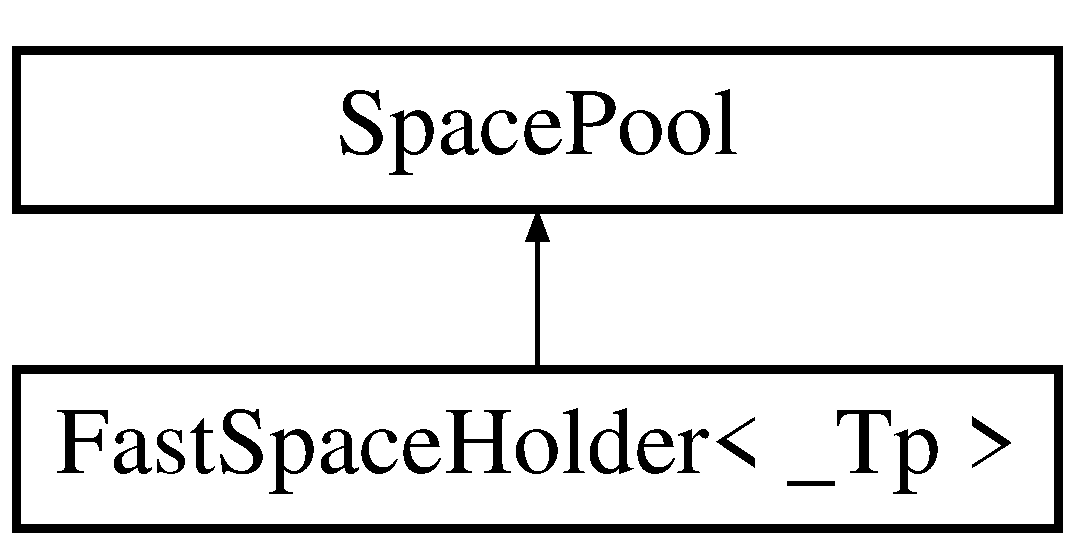
\includegraphics[height=2cm]{classFastSpaceHolder}
\end{center}
\end{figure}
\subsection*{Public Member Functions}
\begin{DoxyCompactItemize}
\item 
{\bfseries FastSpaceHolder} ({\bf SpacePool} \&pool, unsigned prealloc=256)\label{classFastSpaceHolder_a167f87252ec3e7efe1733d7471f873af}

\item 
virtual {\bf $\sim$FastSpaceHolder} ()\label{classFastSpaceHolder_a9159af3587150c073efbdf9767675eae}

\begin{DoxyCompactList}\small\item\em Destructor. \item\end{DoxyCompactList}\item 
\_\-Tp $\ast$ {\bf array} (unsigned n)
\begin{DoxyCompactList}\small\item\em Create array of type \_\-Tp. \item\end{DoxyCompactList}\item 
\_\-Tp $\ast$ {\bf alloc} ()\label{classFastSpaceHolder_a0ad44bb4cc8378a4f5596c523ea1c8a9}

\begin{DoxyCompactList}\small\item\em Allocate space for \_\-Tp. \item\end{DoxyCompactList}\end{DoxyCompactItemize}
\subsection*{Private Member Functions}
\begin{DoxyCompactItemize}
\item 
{\bfseries FastSpaceHolder} ({\bf FastSpaceHolder}$<$ \_\-Tp $>$ \&x, bool)\label{classFastSpaceHolder_a8d48587881491d4aa72aad07e5899a2e}

\end{DoxyCompactItemize}
\subsection*{Private Attributes}
\begin{DoxyCompactItemize}
\item 
\_\-Tp $\ast$ {\bfseries data}\label{classFastSpaceHolder_abb9b40a2bbb5b57766b28c406af250f9}

\end{DoxyCompactItemize}


\subsection{Detailed Description}
\subsubsection*{template$<$class \_\-Tp$>$ class FastSpaceHolder$<$ \_\-Tp $>$}

Fast version, but: it is impossible put into this container something with implicit or explicit ctor/dtor (no virtual functions). 

Definition at line 123 of file RecoUtil.hh.

\subsection{Member Function Documentation}
\index{FastSpaceHolder@{FastSpaceHolder}!array@{array}}
\index{array@{array}!FastSpaceHolder@{FastSpaceHolder}}
\subsubsection[{array}]{\setlength{\rightskip}{0pt plus 5cm}template$<$class \_\-Tp$>$ \_\-Tp$\ast$ {\bf FastSpaceHolder}$<$ \_\-Tp $>$::array (unsigned {\em n})\hspace{0.3cm}{\ttfamily  [inline]}}\label{classFastSpaceHolder_abbfd87752276f2833ed20a1410bfaa74}


Create array of type \_\-Tp. 
\begin{DoxyParams}{Parameters}
\item[{\em n}]size of array \end{DoxyParams}


Definition at line 142 of file RecoUtil.hh.

Referenced by FastSpaceHolder$<$ RSLink $>$::alloc().

The documentation for this class was generated from the following file:\begin{DoxyCompactItemize}
\item 
RecoUtil.hh\end{DoxyCompactItemize}

\section{DeepAnalysis::Group Class Reference}
\label{classDeepAnalysis_1_1Group}\index{DeepAnalysis::Group@{DeepAnalysis::Group}}


Class for general multipurpose grouping.  


{\ttfamily \#include $<$DeepAnalysis.hh$>$}Inheritance diagram for DeepAnalysis::Group::\begin{figure}[H]
\begin{center}
\leavevmode
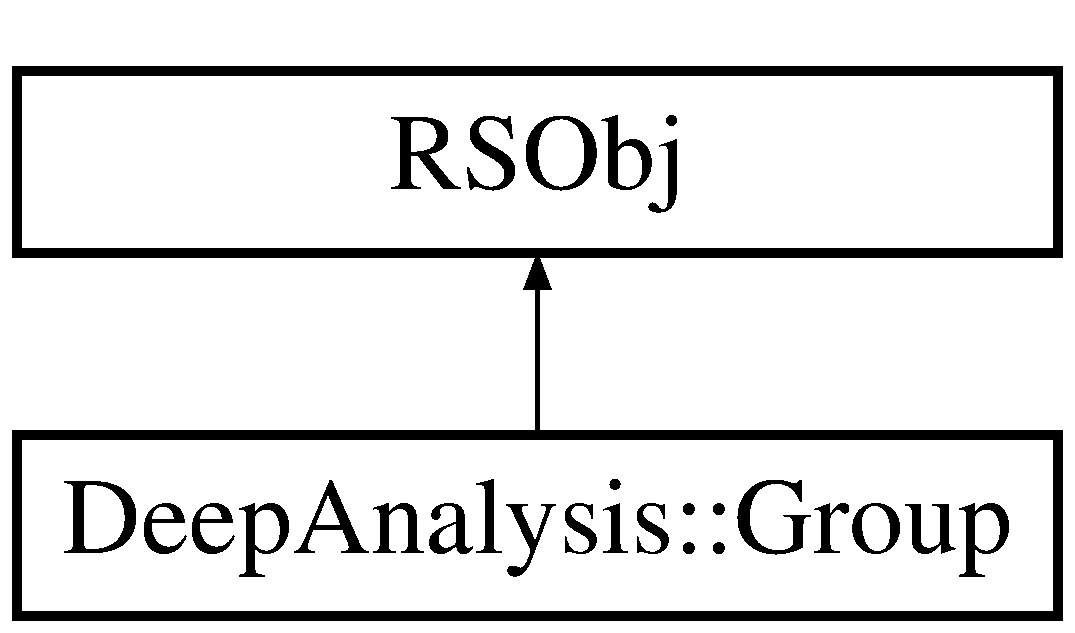
\includegraphics[height=2cm]{classDeepAnalysis_1_1Group}
\end{center}
\end{figure}
\subsection*{Public Member Functions}
\begin{DoxyCompactItemize}
\item 
{\bf Group} ()\label{classDeepAnalysis_1_1Group_a8cd4cf91d461db9ac2ed340a0ed3476c}

\begin{DoxyCompactList}\small\item\em Constructor. \item\end{DoxyCompactList}\end{DoxyCompactItemize}
\subsection*{Static Public Attributes}
\begin{DoxyCompactItemize}
\item 
static const unsigned {\bf RS\_\-TYPE} = 1\label{classDeepAnalysis_1_1Group_af2bcdbabac63b181d06571d7bd4ae010}

\begin{DoxyCompactList}\small\item\em type of \doxyref{RS}{p.}{classRS} object \item\end{DoxyCompactList}\end{DoxyCompactItemize}


\subsection{Detailed Description}
Class for general multipurpose grouping. 

Definition at line 233 of file DeepAnalysis.hh.

The documentation for this class was generated from the following file:\begin{DoxyCompactItemize}
\item 
DeepAnalysis.hh\end{DoxyCompactItemize}

\section{HistogrammPT::HCell Struct Reference}
\label{structHistogrammPT_1_1HCell}\index{HistogrammPT::HCell@{HistogrammPT::HCell}}
\subsection*{Data Fields}
\begin{DoxyCompactItemize}
\item 
double {\bfseries val}\label{structHistogrammPT_1_1HCell_a1feacd0780567226c7270ed8ab7fe784}

\item 
unsigned {\bfseries p\_\-i}\label{structHistogrammPT_1_1HCell_adb761ef250b282c8bd8ea3068462f51b}

\item 
unsigned {\bfseries t\_\-i}\label{structHistogrammPT_1_1HCell_af1baacf510aa664689756a994096a369}

\end{DoxyCompactItemize}


\subsection{Detailed Description}


Definition at line 18 of file HistogrammPT.h.

The documentation for this struct was generated from the following file:\begin{DoxyCompactItemize}
\item 
HistogrammPT.h\end{DoxyCompactItemize}

\section{HistogrammPT Class Reference}
\label{classHistogrammPT}\index{HistogrammPT@{HistogrammPT}}


Histogram class.  


{\ttfamily \#include $<$HistogrammPT.h$>$}Inheritance diagram for HistogrammPT::\begin{figure}[H]
\begin{center}
\leavevmode
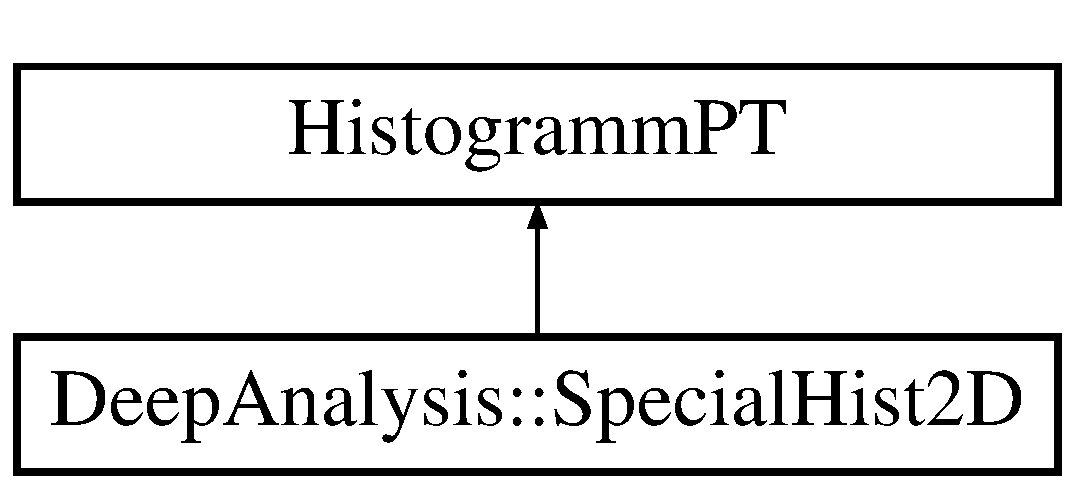
\includegraphics[height=2cm]{classHistogrammPT}
\end{center}
\end{figure}
\subsection*{Data Structures}
\begin{DoxyCompactItemize}
\item 
class {\bf AxisRange}
\begin{DoxyCompactList}\small\item\em Class for axis range. \item\end{DoxyCompactList}\item 
struct {\bf HCell}
\end{DoxyCompactItemize}
\subsection*{Public Member Functions}
\begin{DoxyCompactItemize}
\item 
{\bf HistogrammPT} ()\label{classHistogrammPT_a5eb56dc8f443470d3f2e64261adfcf68}

\begin{DoxyCompactList}\small\item\em Constructor. \item\end{DoxyCompactList}\item 
virtual {\bf $\sim$HistogrammPT} ()\label{classHistogrammPT_a919d7136a094d78a3160f82796ddc390}

\begin{DoxyCompactList}\small\item\em Destructor. \item\end{DoxyCompactList}\item 
virtual bool {\bf Book} (const {\bf MinMaxRange}$<$ double $>$ \&p\_\-lim, const {\bf MinMaxRange}$<$ double $>$ \&t\_\-lim, double \_\-step=0.006)\label{classHistogrammPT_a9f55c84ff9433921ad550901d77a40ce}

\begin{DoxyCompactList}\small\item\em Book histogram. \item\end{DoxyCompactList}\item 
bool {\bf Fill} (const Sphere3D \&sp, double e)\label{classHistogrammPT_a6f2b6c655ae17e89360f57de164c6e67}

\begin{DoxyCompactList}\small\item\em Fill histogram. \item\end{DoxyCompactList}\item 
{\bf HCell} $\ast$ {\bf get} (const Sphere3D \&sp)\label{classHistogrammPT_afde466a0d65f230d96919bdccce12042}

\begin{DoxyCompactList}\small\item\em Get ? \item\end{DoxyCompactList}\item 
{\bf HCell} $\ast$ {\bf get\_\-by\_\-index} (unsigned p\_\-i, unsigned t\_\-i)\label{classHistogrammPT_ab553651b0281a37e947f6326e72f05bf}

\begin{DoxyCompactList}\small\item\em Get by index ? \item\end{DoxyCompactList}\item 
double {\bf get\_\-t} (const {\bf HCell} \&c)\label{classHistogrammPT_a3649641c88c82a93e12339a21de0379d}

\begin{DoxyCompactList}\small\item\em Get t ? \item\end{DoxyCompactList}\item 
double {\bf get\_\-p} (const {\bf HCell} \&c)\label{classHistogrammPT_ac979daa0f17d147c523e2e927617738e}

\begin{DoxyCompactList}\small\item\em Get p ? \item\end{DoxyCompactList}\end{DoxyCompactItemize}
\subsection*{Data Fields}
\begin{DoxyCompactItemize}
\item 
{\bf HCell} $\ast$ {\bfseries c}\label{classHistogrammPT_a7ef98513afbbef61a4a764082dec2dc2}

\item 
unsigned {\bfseries c\_\-count}\label{classHistogrammPT_a253cf428378cf4d9b11aac5344a4e5ed}

\item 
{\bf AxisRange} {\bfseries p}\label{classHistogrammPT_a785c1c78da66f092a60351a39e9661bb}

\item 
{\bf AxisRange} {\bfseries t}\label{classHistogrammPT_a35d3ffa3da74524aeb263212286d2988}

\end{DoxyCompactItemize}


\subsection{Detailed Description}
Histogram class. 

Definition at line 16 of file HistogrammPT.h.

The documentation for this class was generated from the following files:\begin{DoxyCompactItemize}
\item 
HistogrammPT.h\item 
HistogrammPT.cc\end{DoxyCompactItemize}

\section{DeepAnalysis::Hit Class Reference}
\label{classDeepAnalysis_1_1Hit}\index{DeepAnalysis::Hit@{DeepAnalysis::Hit}}


Class for hit: consists of:.  


{\ttfamily \#include $<$DeepAnalysis.hh$>$}Inheritance diagram for DeepAnalysis::Hit::\begin{figure}[H]
\begin{center}
\leavevmode
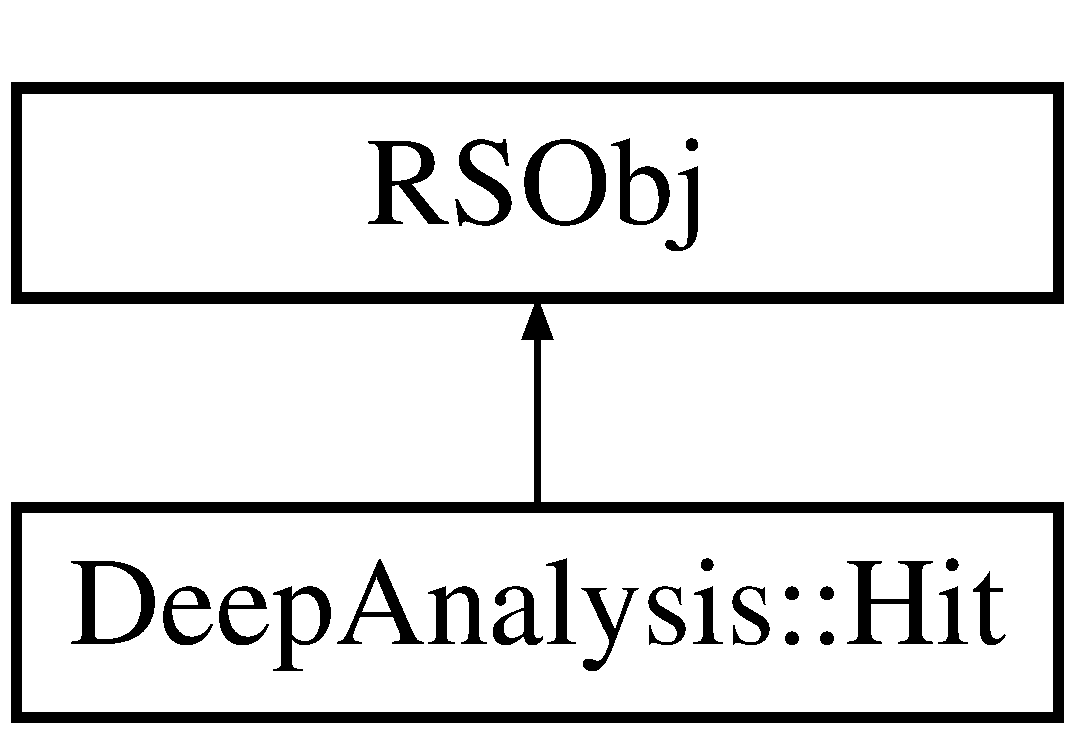
\includegraphics[height=2cm]{classDeepAnalysis_1_1Hit}
\end{center}
\end{figure}
\subsection*{Public Member Functions}
\begin{DoxyCompactItemize}
\item 
{\bf Hit} ()\label{classDeepAnalysis_1_1Hit_ae07a53b3fc9dc9ee0c3a7bcd6dadb748}

\begin{DoxyCompactList}\small\item\em Constructor. \item\end{DoxyCompactList}\item 
void {\bf set} (unsigned \_\-idx, double \_\-x, double \_\-y, double \_\-z, double \_\-am, double \_\-ampl\_\-mip, double \_\-thr, unsigned \_\-lay, int \_\-addr)
\begin{DoxyCompactList}\small\item\em Set hit parameters. \item\end{DoxyCompactList}\item 
void {\bf draw} (unsigned type, unsigned size, unsigned color)
\begin{DoxyCompactList}\small\item\em Draw hit. \item\end{DoxyCompactList}\item 
{\bf KIND} {\bf get\_\-color} ({\bf DeepAnalysis} \&rs)
\begin{DoxyCompactList}\small\item\em Get hit color. \item\end{DoxyCompactList}\end{DoxyCompactItemize}
\subsection*{Data Fields}
\begin{DoxyCompactItemize}
\item 
unsigned {\bf idx}\label{classDeepAnalysis_1_1Hit_adcc608658d5021b8acfd56f34d2e57cc}

\begin{DoxyCompactList}\small\item\em index in input hits \item\end{DoxyCompactList}\item 
Point3D {\bf cartesianPoint}\label{classDeepAnalysis_1_1Hit_a4be7f547d9bb071d195dbbcdbc8fe900}

\begin{DoxyCompactList}\small\item\em cartesian coordinates \item\end{DoxyCompactList}\item 
Sphere3D {\bf sphere3d}\label{classDeepAnalysis_1_1Hit_af2fa1f58d38c3a02f006f8b5289b7648}

\begin{DoxyCompactList}\small\item\em spherical coordinates \item\end{DoxyCompactList}\item 
double {\bf amplGeV}\label{classDeepAnalysis_1_1Hit_a3b8f817d02b3171fdb57c997ee9a558c}

\begin{DoxyCompactList}\small\item\em amplitude [GeV] \item\end{DoxyCompactList}\item 
double {\bf ampl\_\-mip}\label{classDeepAnalysis_1_1Hit_ae28b50dafae6721b055170d2d367c956}

\begin{DoxyCompactList}\small\item\em amplitude in MIPs \item\end{DoxyCompactList}\item 
double {\bf thr}\label{classDeepAnalysis_1_1Hit_a4dab2d64d7e398e42b8cb74f2bbb0fbc}

\begin{DoxyCompactList}\small\item\em threshold in MIPs \item\end{DoxyCompactList}\item 
unsigned {\bf lay}\label{classDeepAnalysis_1_1Hit_a31a55598c143d18d3443365e496e7515}

\begin{DoxyCompactList}\small\item\em layer number \item\end{DoxyCompactList}\item 
int {\bf addr}\label{classDeepAnalysis_1_1Hit_a8a8f5aae460bf9ba23eff1066aa72a99}

\begin{DoxyCompactList}\small\item\em address in initial event array \item\end{DoxyCompactList}\end{DoxyCompactItemize}
\subsection*{Static Public Attributes}
\begin{DoxyCompactItemize}
\item 
static const unsigned {\bf RS\_\-TYPE} = 0\label{classDeepAnalysis_1_1Hit_a0da168f06fb6b3d48524db3f3b226d47}

\begin{DoxyCompactList}\small\item\em type of \doxyref{RS}{p.}{classRS} object \item\end{DoxyCompactList}\end{DoxyCompactItemize}


\subsection{Detailed Description}
Class for hit: consists of:. 

Definition at line 170 of file DeepAnalysis.hh.

\subsection{Member Function Documentation}
\index{DeepAnalysis::Hit@{DeepAnalysis::Hit}!draw@{draw}}
\index{draw@{draw}!DeepAnalysis::Hit@{DeepAnalysis::Hit}}
\subsubsection[{draw}]{\setlength{\rightskip}{0pt plus 5cm}void DeepAnalysis::Hit::draw (unsigned {\em type}, \/  unsigned {\em size}, \/  unsigned {\em color})\hspace{0.3cm}{\ttfamily  [inline]}}\label{classDeepAnalysis_1_1Hit_a5ac3851b0250e454434733fd18923a56}


Draw hit. 
\begin{DoxyParams}{Parameters}
\item[{\em type}]hit type \item[{\em size}]size of point/size of cross \item[{\em color}]color n RGB form (e.g. 0xff0000 is RED) \end{DoxyParams}


Definition at line 216 of file DeepAnalysis.hh.\index{DeepAnalysis::Hit@{DeepAnalysis::Hit}!get\_\-color@{get\_\-color}}
\index{get\_\-color@{get\_\-color}!DeepAnalysis::Hit@{DeepAnalysis::Hit}}
\subsubsection[{get\_\-color}]{\setlength{\rightskip}{0pt plus 5cm}{\bf DeepAnalysis::KIND} DeepAnalysis::Hit::get\_\-color ({\bf DeepAnalysis} \& {\em deepAnalysis})\hspace{0.3cm}{\ttfamily  [inline]}}\label{classDeepAnalysis_1_1Hit_a78087dea3baa8b9fd1ffcf99c820a496}


Get hit color. 
\begin{DoxyParams}{Parameters}
\item[{\em deepAnalysis}]\end{DoxyParams}


Definition at line 1633 of file DeepAnalysis.hh.

References DeepAnalysis::EM, DeepAnalysis::HAD, DeepAnalysis::kind, DeepAnalysis::NEUTR, and DeepAnalysis::TRK.\index{DeepAnalysis::Hit@{DeepAnalysis::Hit}!set@{set}}
\index{set@{set}!DeepAnalysis::Hit@{DeepAnalysis::Hit}}
\subsubsection[{set}]{\setlength{\rightskip}{0pt plus 5cm}void DeepAnalysis::Hit::set (unsigned {\em \_\-idx}, \/  double {\em \_\-x}, \/  double {\em \_\-y}, \/  double {\em \_\-z}, \/  double {\em \_\-am}, \/  double {\em \_\-ampl\_\-mip}, \/  double {\em \_\-thr}, \/  unsigned {\em \_\-lay}, \/  int {\em \_\-addr})\hspace{0.3cm}{\ttfamily  [inline]}}\label{classDeepAnalysis_1_1Hit_aee70433682ef0e0b4d33f374d8686fb8}


Set hit parameters. 
\begin{DoxyParams}{Parameters}
\item[{\em \_\-idx}]index in input hits \item[{\em \_\-x}]x-\/coordinate \item[{\em \_\-y}]y-\/coordinate \item[{\em \_\-z}]z-\/coordinate \item[{\em \_\-am}]amplitude (in GeV) \item[{\em \_\-ampl\_\-mip}]amplitude (in MIPs) \item[{\em \_\-thr}]threshold in MIPs \item[{\em \_\-lay}]layer number \item[{\em \_\-addr}]address in initial event array \end{DoxyParams}


Definition at line 198 of file DeepAnalysis.hh.

References addr, ampl\_\-mip, amplGeV, cartesianPoint, idx, lay, sphere3d, and thr.

Referenced by DeepAnalysis::add\_\-hit().

The documentation for this class was generated from the following file:\begin{DoxyCompactItemize}
\item 
DeepAnalysis.hh\end{DoxyCompactItemize}

\section{DeepAnalysis::HitGroup Class Reference}
\label{classDeepAnalysis_1_1HitGroup}\index{DeepAnalysis::HitGroup@{DeepAnalysis::HitGroup}}


This class is not a cluster, but this is as it said in name -\/-\/ \doxyref{Group}{p.}{classDeepAnalysis_1_1Group} of Hits, that has a boundaries in 3-\/D cartesian coordinate system and spherical coordinate system, center of gravity and whole energy.  


{\ttfamily \#include $<$DeepAnalysis.hh$>$}Inheritance diagram for DeepAnalysis::HitGroup::\begin{figure}[H]
\begin{center}
\leavevmode
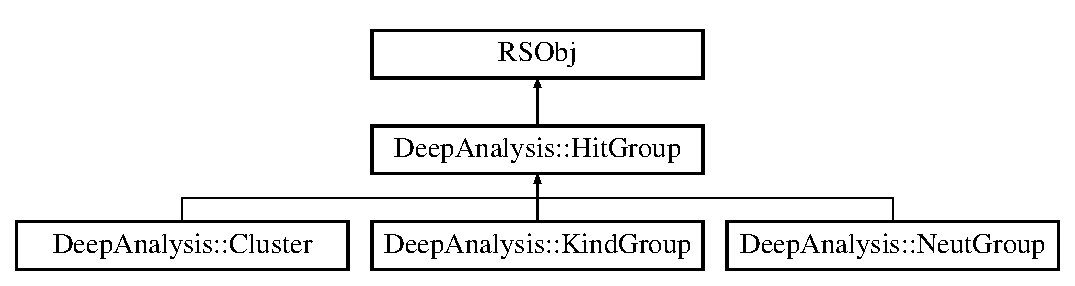
\includegraphics[height=3cm]{classDeepAnalysis_1_1HitGroup}
\end{center}
\end{figure}
\subsection*{Public Member Functions}
\begin{DoxyCompactItemize}
\item 
{\bf HitGroup} ()\label{classDeepAnalysis_1_1HitGroup_ad5d6fbecb4b545154e96c6e7645753fa}

\begin{DoxyCompactList}\small\item\em Constructor. \item\end{DoxyCompactList}\item 
void {\bf calc\_\-stat} ()\label{classDeepAnalysis_1_1HitGroup_aaf039464568eec388ec2aac8ec7de56a}

\begin{DoxyCompactList}\small\item\em Calculate initial statistics of this \doxyref{Group}{p.}{classDeepAnalysis_1_1Group} of Hits. \item\end{DoxyCompactList}\item 
void {\bf draw} (unsigned type, unsigned size, unsigned color)
\begin{DoxyCompactList}\small\item\em Draw hits. \item\end{DoxyCompactList}\end{DoxyCompactItemize}
\subsection*{Data Fields}
\begin{DoxyCompactItemize}
\item 
Vector3D {\bf centerOfGravity}
\begin{DoxyCompactList}\small\item\em center of gravity (X\_\-clust. \item\end{DoxyCompactList}\item 
double {\bf energySum}\label{classDeepAnalysis_1_1HitGroup_a4e559ed6aea2b05f50209579ed04565f}

\begin{DoxyCompactList}\small\item\em sum of energy \item\end{DoxyCompactList}\item 
{\bf MinMaxRange}$<$ int $>$ {\bf layer\_\-g}\label{classDeepAnalysis_1_1HitGroup_a7889f649bed4ae5eeabbdb6611eef5e2}

\begin{DoxyCompactList}\small\item\em layer \item\end{DoxyCompactList}\item 
{\bf MinMaxRange}$<$ double $>$ {\bf radius\_\-g}\label{classDeepAnalysis_1_1HitGroup_a79beed76651f6412ede510c4d185a3ce}

\begin{DoxyCompactList}\small\item\em radius \item\end{DoxyCompactList}\item 
{\bf MinMaxRange}$<$ double $>$ {\bf theta\_\-g}\label{classDeepAnalysis_1_1HitGroup_a8d1e2c21b771032f2554a68f9e6491b9}

\begin{DoxyCompactList}\small\item\em theta \item\end{DoxyCompactList}\item 
{\bf MinMaxRange}$<$ double $>$ {\bf phi\_\-g}\label{classDeepAnalysis_1_1HitGroup_a82f638c2e9a04adfa458debbe6fcf4d1}

\begin{DoxyCompactList}\small\item\em phi \item\end{DoxyCompactList}\end{DoxyCompactItemize}
\subsection*{Static Public Attributes}
\begin{DoxyCompactItemize}
\item 
static const unsigned {\bf RS\_\-TYPE} = 2\label{classDeepAnalysis_1_1HitGroup_a71e1f65d89bff32b0729454b1027b9ea}

\begin{DoxyCompactList}\small\item\em type of \doxyref{RS}{p.}{classRS} object \item\end{DoxyCompactList}\end{DoxyCompactItemize}


\subsection{Detailed Description}
This class is not a cluster, but this is as it said in name -\/-\/ \doxyref{Group}{p.}{classDeepAnalysis_1_1Group} of Hits, that has a boundaries in 3-\/D cartesian coordinate system and spherical coordinate system, center of gravity and whole energy. 

Definition at line 245 of file DeepAnalysis.hh.

\subsection{Member Function Documentation}
\index{DeepAnalysis::HitGroup@{DeepAnalysis::HitGroup}!draw@{draw}}
\index{draw@{draw}!DeepAnalysis::HitGroup@{DeepAnalysis::HitGroup}}
\subsubsection[{draw}]{\setlength{\rightskip}{0pt plus 5cm}void DeepAnalysis::HitGroup::draw (unsigned {\em type}, \/  unsigned {\em size}, \/  unsigned {\em color})\hspace{0.3cm}{\ttfamily  [inline]}}\label{classDeepAnalysis_1_1HitGroup_a66d1fe2165387c9b25990aa369a7bc51}


Draw hits. 
\begin{DoxyParams}{Parameters}
\item[{\em type}]hit type \item[{\em size}]size of point/size of cross \item[{\em color}]color n RGB form (e.g. 0xff0000 is RED) \end{DoxyParams}


Definition at line 287 of file DeepAnalysis.hh.

\subsection{Field Documentation}
\index{DeepAnalysis::HitGroup@{DeepAnalysis::HitGroup}!centerOfGravity@{centerOfGravity}}
\index{centerOfGravity@{centerOfGravity}!DeepAnalysis::HitGroup@{DeepAnalysis::HitGroup}}
\subsubsection[{centerOfGravity}]{\setlength{\rightskip}{0pt plus 5cm}Vector3D {\bf DeepAnalysis::HitGroup::centerOfGravity}}\label{classDeepAnalysis_1_1HitGroup_a66e5d49bbb2fd5737e2b43872461d59f}


center of gravity (X\_\-clust. .., xs...) 

Definition at line 251 of file DeepAnalysis.hh.

Referenced by DeepAnalysis::Cluster::calc\_\-prop(), calc\_\-stat(), DeepAnalysis::Cluster::draw\_\-ellipse(), DeepAnalysis::Cluster::draw\_\-star(), DeepAnalysis::Cluster::inertia\_\-3d(), and DeepAnalysis::Cluster::rotate\_\-point().

The documentation for this class was generated from the following file:\begin{DoxyCompactItemize}
\item 
DeepAnalysis.hh\end{DoxyCompactItemize}

\section{DeepAnalysis::JoinGroup Class Reference}
\label{classDeepAnalysis_1_1JoinGroup}\index{DeepAnalysis::JoinGroup@{DeepAnalysis::JoinGroup}}


Class for joining groups (juts a working intermediate class) (for \doxyref{cluster\_\-join}{p.}{classDeepAnalysis_a11f0ad635e5acf4b82c36170b9db6293} method).  


{\ttfamily \#include $<$DeepAnalysis.hh$>$}Inheritance diagram for DeepAnalysis::JoinGroup::\begin{figure}[H]
\begin{center}
\leavevmode
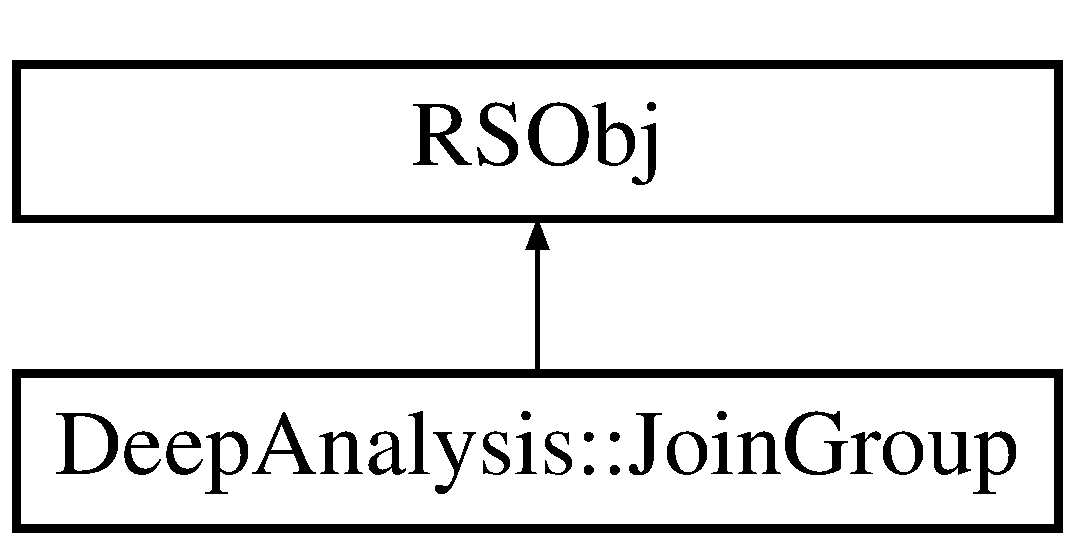
\includegraphics[height=2cm]{classDeepAnalysis_1_1JoinGroup}
\end{center}
\end{figure}
\subsection*{Public Member Functions}
\begin{DoxyCompactItemize}
\item 
{\bf JoinGroup} ()\label{classDeepAnalysis_1_1JoinGroup_a04b24b0c31f7e5c032b8b9cb1f527206}

\begin{DoxyCompactList}\small\item\em Constructor. \item\end{DoxyCompactList}\end{DoxyCompactItemize}
\subsection*{Static Public Attributes}
\begin{DoxyCompactItemize}
\item 
static const unsigned {\bf RS\_\-TYPE} = 5\label{classDeepAnalysis_1_1JoinGroup_aab02e64d0a49fc1e08169cbc64484c59}

\begin{DoxyCompactList}\small\item\em type of \doxyref{RS}{p.}{classRS} object \item\end{DoxyCompactList}\end{DoxyCompactItemize}


\subsection{Detailed Description}
Class for joining groups (juts a working intermediate class) (for \doxyref{cluster\_\-join}{p.}{classDeepAnalysis_a11f0ad635e5acf4b82c36170b9db6293} method). 

Definition at line 314 of file DeepAnalysis.hh.

The documentation for this class was generated from the following file:\begin{DoxyCompactItemize}
\item 
DeepAnalysis.hh\end{DoxyCompactItemize}

\section{DeepAnalysis::KindGroup Class Reference}
\label{classDeepAnalysis_1_1KindGroup}\index{DeepAnalysis::KindGroup@{DeepAnalysis::KindGroup}}


This class has a represents of RGB types of Groups.  


{\ttfamily \#include $<$DeepAnalysis.hh$>$}Inheritance diagram for DeepAnalysis::KindGroup::\begin{figure}[H]
\begin{center}
\leavevmode
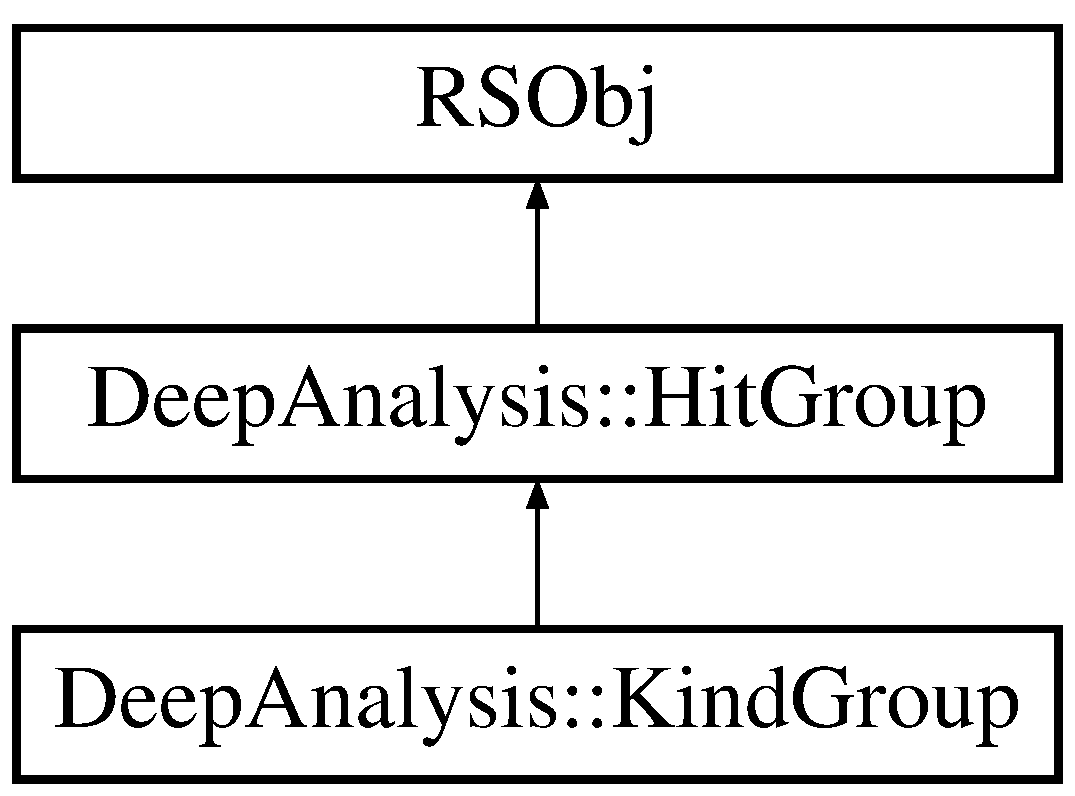
\includegraphics[height=3cm]{classDeepAnalysis_1_1KindGroup}
\end{center}
\end{figure}
\subsection*{Public Member Functions}
\begin{DoxyCompactItemize}
\item 
{\bf KindGroup} ()\label{classDeepAnalysis_1_1KindGroup_a687c4ae2fadfbf1e479b7f1ea84d150b}

\begin{DoxyCompactList}\small\item\em Constructor. \item\end{DoxyCompactList}\end{DoxyCompactItemize}
\subsection*{Static Public Attributes}
\begin{DoxyCompactItemize}
\item 
static const unsigned {\bf RS\_\-TYPE} = 3\label{classDeepAnalysis_1_1KindGroup_aa29cbaca3544cc266487b10229c794c4}

\begin{DoxyCompactList}\small\item\em type of \doxyref{RS}{p.}{classRS} object \item\end{DoxyCompactList}\end{DoxyCompactItemize}


\subsection{Detailed Description}
This class has a represents of RGB types of Groups. 

Definition at line 297 of file DeepAnalysis.hh.

The documentation for this class was generated from the following file:\begin{DoxyCompactItemize}
\item 
DeepAnalysis.hh\end{DoxyCompactItemize}

\section{MinMaxRange$<$ \_\-T $>$ Class Template Reference}
\label{classMinMaxRange}\index{MinMaxRange@{MinMaxRange}}
Inheritance diagram for MinMaxRange$<$ \_\-T $>$::\begin{figure}[H]
\begin{center}
\leavevmode
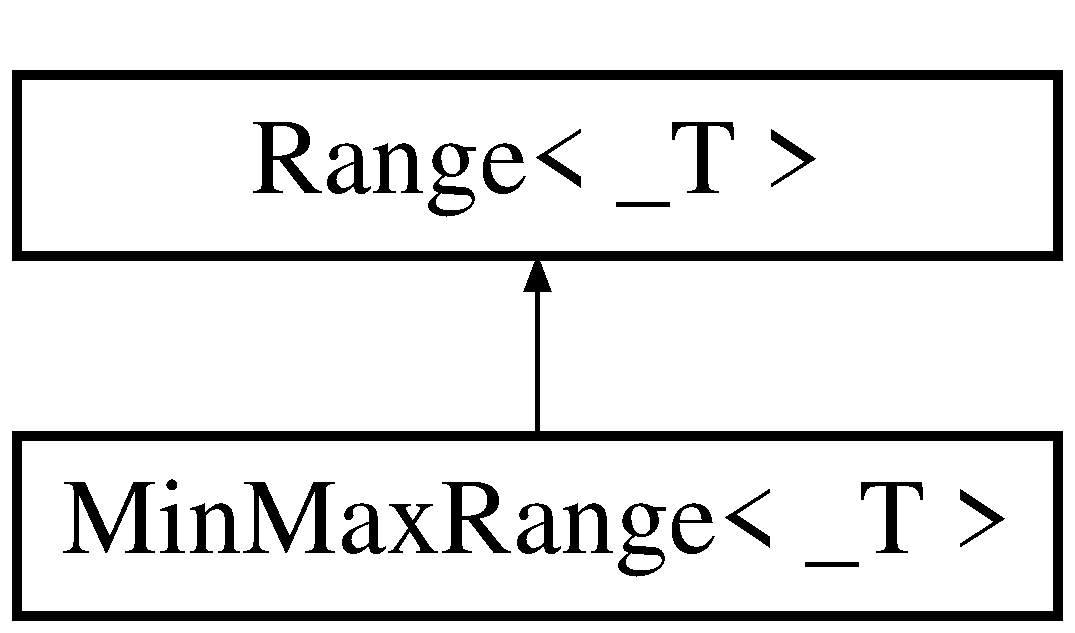
\includegraphics[height=2cm]{classMinMaxRange}
\end{center}
\end{figure}
\subsection*{Public Member Functions}
\begin{DoxyCompactItemize}
\item 
void {\bf set} (\_\-T value)\label{classMinMaxRange_a16b7b6c4aaf960f65df1f168e9b43e06}

\begin{DoxyCompactList}\small\item\em Add value. \item\end{DoxyCompactList}\item 
void {\bfseries init} ()\label{classMinMaxRange_a62a97ff19a090c75c97945983bc56e7a}

\end{DoxyCompactItemize}


\subsection{Detailed Description}
\subsubsection*{template$<$class \_\-T$>$ class MinMaxRange$<$ \_\-T $>$}



Definition at line 241 of file B\_\-Util\_\-DA.h.

The documentation for this class was generated from the following file:\begin{DoxyCompactItemize}
\item 
B\_\-Util\_\-DA.h\end{DoxyCompactItemize}

\section{DeepAnalysis::NeutGroup Class Reference}
\label{classDeepAnalysis_1_1NeutGroup}\index{DeepAnalysis::NeutGroup@{DeepAnalysis::NeutGroup}}


Neutrons group (specific for technical reasons).  


{\ttfamily \#include $<$DeepAnalysis.hh$>$}Inheritance diagram for DeepAnalysis::NeutGroup::\begin{figure}[H]
\begin{center}
\leavevmode
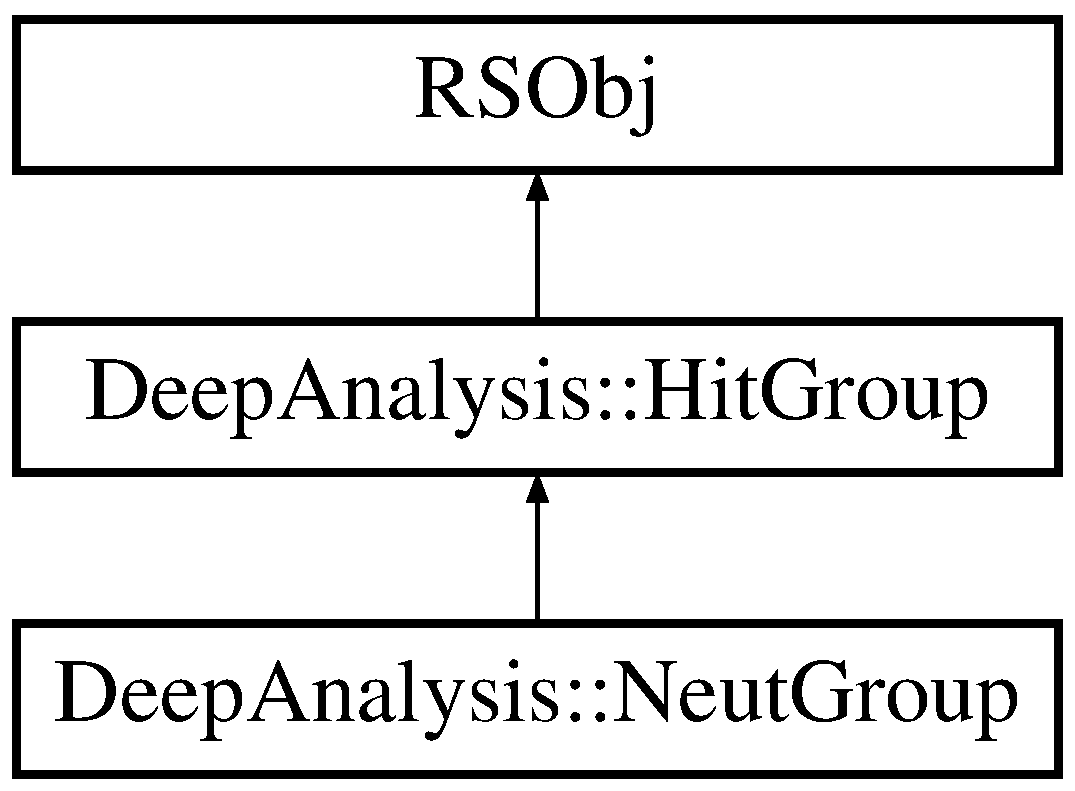
\includegraphics[height=3cm]{classDeepAnalysis_1_1NeutGroup}
\end{center}
\end{figure}
\subsection*{Public Member Functions}
\begin{DoxyCompactItemize}
\item 
{\bf NeutGroup} ()\label{classDeepAnalysis_1_1NeutGroup_a316c2e8aca173e9f0f3b71bef95f79f6}

\begin{DoxyCompactList}\small\item\em Constructor. \item\end{DoxyCompactList}\end{DoxyCompactItemize}
\subsection*{Static Public Attributes}
\begin{DoxyCompactItemize}
\item 
static const unsigned {\bf RS\_\-TYPE} = 4\label{classDeepAnalysis_1_1NeutGroup_a21b1c1fffe547b68fc24ec73bc1025a7}

\begin{DoxyCompactList}\small\item\em type of \doxyref{RS}{p.}{classRS} object \item\end{DoxyCompactList}\end{DoxyCompactItemize}


\subsection{Detailed Description}
Neutrons group (specific for technical reasons). 

Definition at line 306 of file DeepAnalysis.hh.

The documentation for this class was generated from the following file:\begin{DoxyCompactItemize}
\item 
DeepAnalysis.hh\end{DoxyCompactItemize}

\section{Range$<$ \_\-T $>$ Class Template Reference}
\label{classRange}\index{Range@{Range}}
Inheritance diagram for Range$<$ \_\-T $>$::\begin{figure}[H]
\begin{center}
\leavevmode
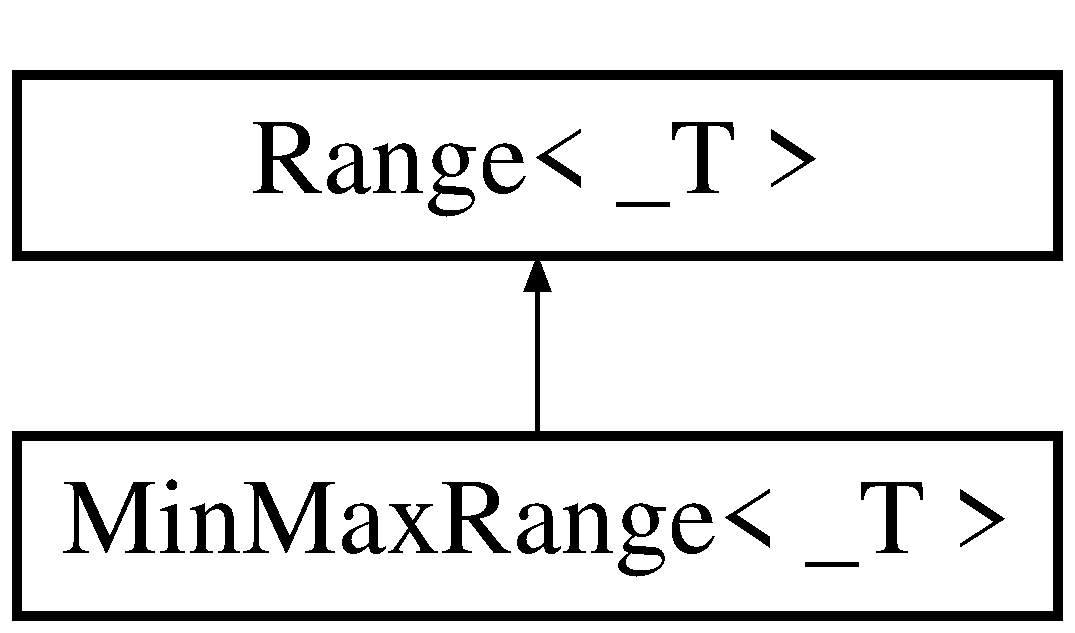
\includegraphics[height=2cm]{classRange}
\end{center}
\end{figure}
\subsection*{Public Member Functions}
\begin{DoxyCompactItemize}
\item 
{\bfseries Range} (\_\-T \_\-min, \_\-T \_\-max)\label{classRange_aaa73dd31c0c629a02e214f6db438e5e1}

\item 
{\bfseries Range} (\_\-T \_\-minmax)\label{classRange_a09e1bb3d87e276a48a855a22602ef677}

\item 
void {\bfseries extend} (\_\-T diff)\label{classRange_ae24bebe307766cef33c471dc8883b7a0}

\item 
\_\-T {\bfseries range} () const \label{classRange_ad24d5d2bcbcaf468dbc9b639cb66ca2c}

\item 
bool {\bfseries inrange} (const \_\-T value) const \label{classRange_aa775f3e2c83c494507c17b9938f04a44}

\item 
bool {\bfseries valid} () const \label{classRange_abdc59f930d73c924f28ba23b83b3ac41}

\end{DoxyCompactItemize}
\subsection*{Data Fields}
\begin{DoxyCompactItemize}
\item 
\_\-T {\bf max}\label{classRange_a3f5b42cf64810fc334f805fd6f146197}

\begin{DoxyCompactList}\small\item\em maximum value \item\end{DoxyCompactList}\item 
\_\-T {\bf min}\label{classRange_ab7904596c5b8a52eb5e6671ed8ca942d}

\begin{DoxyCompactList}\small\item\em minimum value \item\end{DoxyCompactList}\end{DoxyCompactItemize}


\subsection{Detailed Description}
\subsubsection*{template$<$class \_\-T$>$ class Range$<$ \_\-T $>$}



Definition at line 215 of file B\_\-Util\_\-DA.h.

The documentation for this class was generated from the following file:\begin{DoxyCompactItemize}
\item 
B\_\-Util\_\-DA.h\end{DoxyCompactItemize}

\section{RS Class Reference}
\label{classRS}\index{RS@{RS}}


Something.  


{\ttfamily \#include $<$RecoUtil.hh$>$}Inheritance diagram for RS::\begin{figure}[H]
\begin{center}
\leavevmode
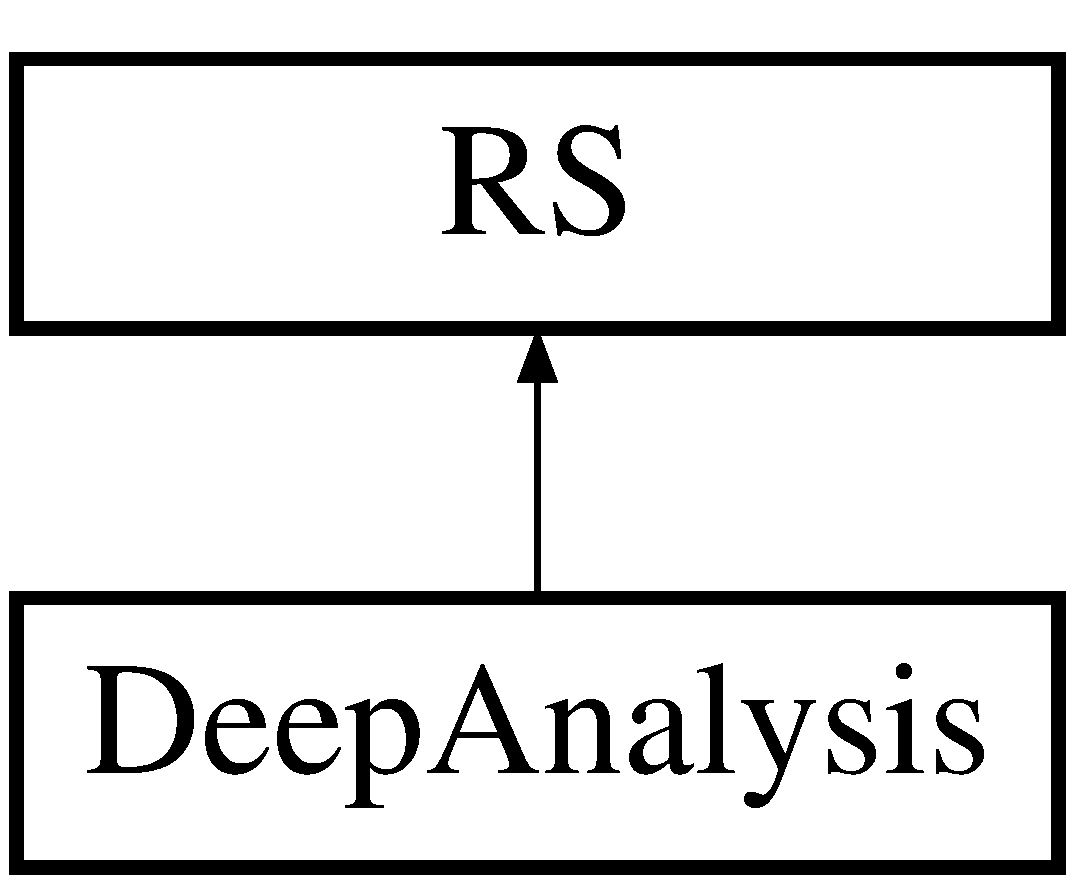
\includegraphics[height=2cm]{classRS}
\end{center}
\end{figure}
\subsection*{Public Member Functions}
\begin{DoxyCompactItemize}
\item 
{\footnotesize template$<$class \_\-Tp $>$ }\\\_\-Tp $\ast$ {\bfseries alloc} ()\label{classRS_ac77e877da97d17cadbaa0684b6f10c58}

\item 
void {\bfseries unlink} ({\bf RSObj} $\ast$cld, {\bf RSObj} $\ast$prt)\label{classRS_add62222b166ede30bc242cf115059409}

\item 
void {\bfseries unlink} ({\bf RSObj} $\ast$obj)\label{classRS_af0e279ecf61559bc9719285a2a8fef0b}

\item 
void {\bfseries prepend} ({\bf RSObj} $\ast$cld, {\bf RSObj} $\ast$prt)\label{classRS_a0135830c1eef7c9c8666fc5ee98e5b2b}

\item 
void {\bfseries append} ({\bf RSObj} $\ast$cld, {\bf RSObj} $\ast$prt)\label{classRS_a1d9b09c9ad252a5211efe8009c205ac8}

\item 
{\footnotesize template$<$class \_\-Tp $>$ }\\void {\bfseries SortChildren} ({\bf RSObj} $\ast$obj, int($\ast$compare)(const \_\-Tp $\ast$$\ast$, const \_\-Tp $\ast$$\ast$))\label{classRS_a4888c2bb20b2ee1b1fd91d8b912ee7be}

\end{DoxyCompactItemize}
\subsection*{Data Fields}
\begin{DoxyCompactItemize}
\item 
void $\ast$ {\bfseries obj\_\-pool} [32]\label{classRS_aff4e259ae5012e7916f8e52f6755b413}

\item 
{\bf SpacePool} {\bfseries pool}\label{classRS_ac985cded70310952e9b69aa86e0d6525}

\end{DoxyCompactItemize}
\subsection*{Private Attributes}
\begin{DoxyCompactItemize}
\item 
{\bf FastSpaceHolder}$<$ {\bf RSLink} $>$ $\ast$ {\bfseries link\_\-pool}\label{classRS_a4fc74f14d80ae96f630d0be93ff418aa}

\item 
{\bf FastSpaceHolder}$<$ {\bf RSLinkGroup} $>$ $\ast$ {\bfseries link\_\-group\_\-pool}\label{classRS_a34c8f9118059702b3a88b53e4ddfe5d6}

\end{DoxyCompactItemize}


\subsection{Detailed Description}
Something. 

Definition at line 311 of file RecoUtil.hh.

The documentation for this class was generated from the following file:\begin{DoxyCompactItemize}
\item 
RecoUtil.hh\end{DoxyCompactItemize}

\section{RSDeepIterator$<$ \_\-Tp $>$ Class Template Reference}
\label{classRSDeepIterator}\index{RSDeepIterator@{RSDeepIterator}}
Inheritance diagram for RSDeepIterator$<$ \_\-Tp $>$::\begin{figure}[H]
\begin{center}
\leavevmode
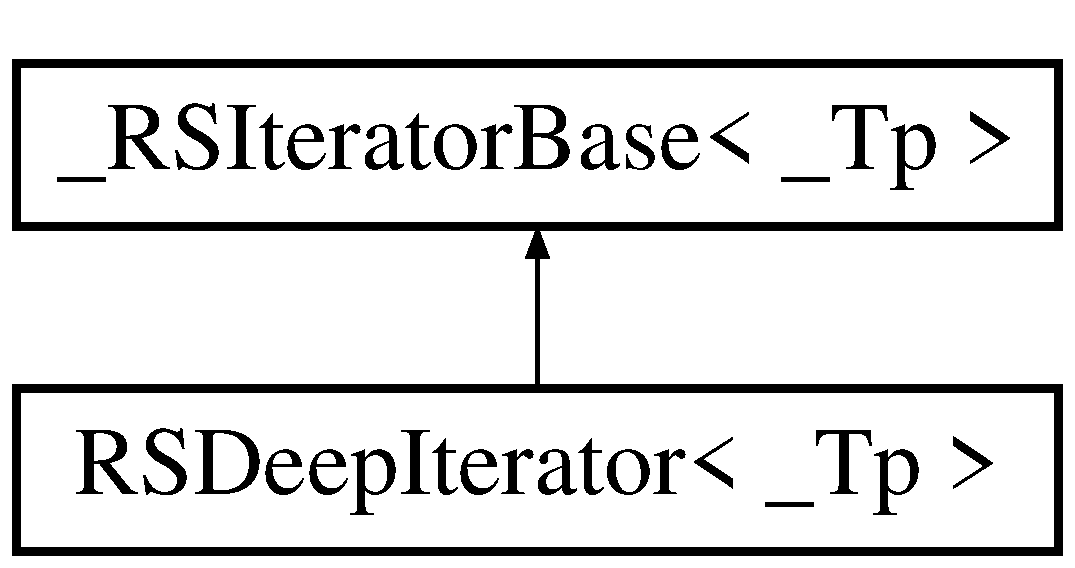
\includegraphics[height=2cm]{classRSDeepIterator}
\end{center}
\end{figure}
\subsection*{Public Member Functions}
\begin{DoxyCompactItemize}
\item 
{\bfseries RSDeepIterator} ({\bf RSObj} $\ast$\_\-root, int \_\-max\_\-depth=31)\label{classRSDeepIterator_a16162dbbc162fe7716f6bd74a8d4b2c1}

\item 
bool {\bfseries next} ()\label{classRSDeepIterator_aae0a761b0662e11ce2e2b1c909c6d74f}

\end{DoxyCompactItemize}
\subsection*{Private Member Functions}
\begin{DoxyCompactItemize}
\item 
bool {\bfseries \_\-find\_\-first} (unsigned depth)\label{classRSDeepIterator_ac7293f782dda57e237f51f389ee58fa5}

\item 
void {\bfseries \_\-find\_\-next} ()\label{classRSDeepIterator_ac7c7e863c1e7a867c66a45e81cd948cb}

\end{DoxyCompactItemize}
\subsection*{Private Attributes}
\begin{DoxyCompactItemize}
\item 
unsigned {\bfseries max\_\-depth}\label{classRSDeepIterator_ac7e35d0bc6564ced0fba22e897de2077}

\item 
unsigned {\bfseries cdepth}\label{classRSDeepIterator_ab9649bd60bd774285389d9e58aa7433f}

\item 
{\bf RSLinkGroup} $\ast$ {\bfseries clg} [32]\label{classRSDeepIterator_ada447dc246ba74d344c20dec4d706345}

\item 
{\bf RSLink} $\ast$ {\bfseries clnk} [32]\label{classRSDeepIterator_a3c744e3562ff2491e8c4c95e7153cfab}

\end{DoxyCompactItemize}


\subsection{Detailed Description}
\subsubsection*{template$<$class \_\-Tp$>$ class RSDeepIterator$<$ \_\-Tp $>$}



Definition at line 540 of file RecoUtil.hh.

The documentation for this class was generated from the following file:\begin{DoxyCompactItemize}
\item 
RecoUtil.hh\end{DoxyCompactItemize}

\section{RSIterator$<$ \_\-Tp $>$ Class Template Reference}
\label{classRSIterator}\index{RSIterator@{RSIterator}}
Inheritance diagram for RSIterator$<$ \_\-Tp $>$::\begin{figure}[H]
\begin{center}
\leavevmode
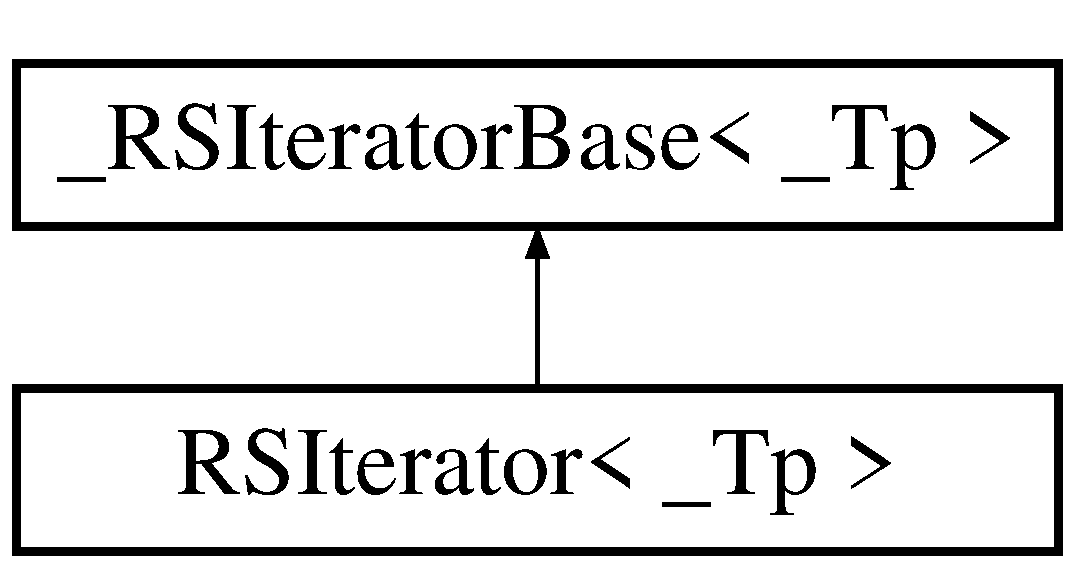
\includegraphics[height=2cm]{classRSIterator}
\end{center}
\end{figure}
\subsection*{Public Member Functions}
\begin{DoxyCompactItemize}
\item 
{\bfseries RSIterator} ({\bf RSObj} $\ast$\_\-root)\label{classRSIterator_a45c2bba6dbcadf418450aa27ac07cc66}

\item 
bool {\bfseries next} ()\label{classRSIterator_a218c6e684151e411d51be7f09ef78cd1}

\item 
bool {\bfseries valid} () const \label{classRSIterator_a0a764a811e825fc874152ba072abb6bf}

\end{DoxyCompactItemize}
\subsection*{Private Member Functions}
\begin{DoxyCompactItemize}
\item 
void {\bfseries \_\-find\_\-first} ()\label{classRSIterator_a0eecc732b9c10c1b66cfe6254eac0a62}

\item 
void {\bfseries \_\-find\_\-next} ()\label{classRSIterator_af89e993afce640fe59ed3a1d34cd35d5}

\end{DoxyCompactItemize}


\subsection{Detailed Description}
\subsubsection*{template$<$class \_\-Tp$>$ class RSIterator$<$ \_\-Tp $>$}



Definition at line 463 of file RecoUtil.hh.

The documentation for this class was generated from the following file:\begin{DoxyCompactItemize}
\item 
RecoUtil.hh\end{DoxyCompactItemize}

\section{RSLink Class Reference}
\label{classRSLink}\index{RSLink@{RSLink}}
Inheritance diagram for RSLink::\begin{figure}[H]
\begin{center}
\leavevmode
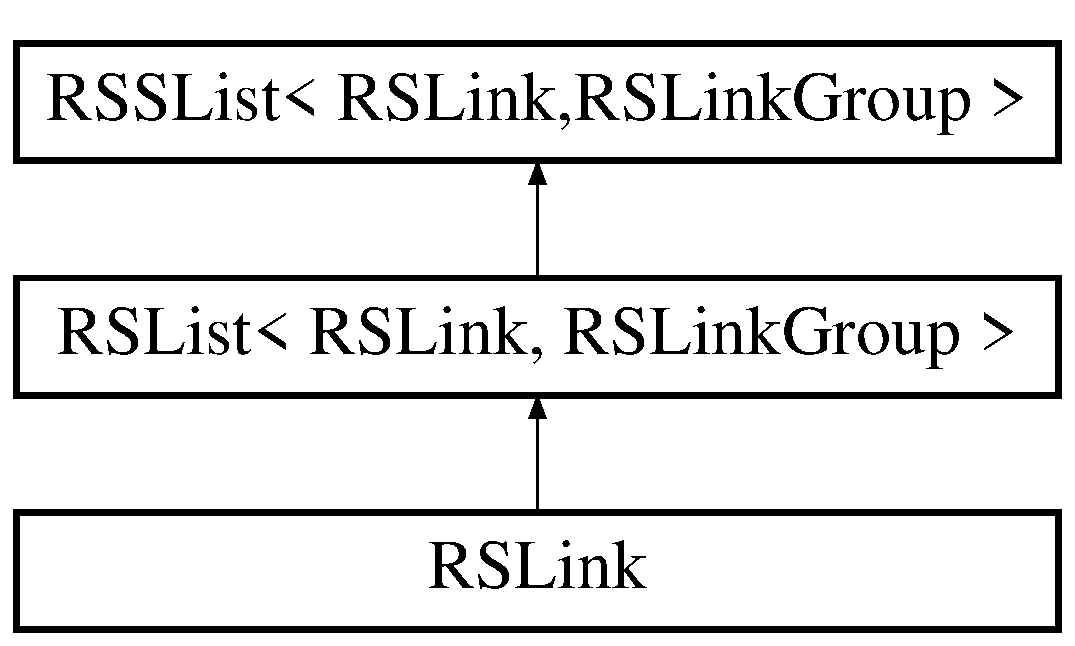
\includegraphics[height=3cm]{classRSLink}
\end{center}
\end{figure}
\subsection*{Data Fields}
\begin{DoxyCompactItemize}
\item 
{\bf RSObj} $\ast$ {\bfseries obj}\label{classRSLink_a3f082748a6ac0ba61e9b49702cde4951}

\item 
{\bf RSLink} $\ast$ {\bfseries nxt\_\-lnk}\label{classRSLink_a8aab02c64d735f834952fd298e805074}

\end{DoxyCompactItemize}


\subsection{Detailed Description}


Definition at line 193 of file RecoUtil.hh.

The documentation for this class was generated from the following file:\begin{DoxyCompactItemize}
\item 
RecoUtil.hh\end{DoxyCompactItemize}

\section{RSLinkGroup Class Reference}
\label{classRSLinkGroup}\index{RSLinkGroup@{RSLinkGroup}}
Inheritance diagram for RSLinkGroup::\begin{figure}[H]
\begin{center}
\leavevmode
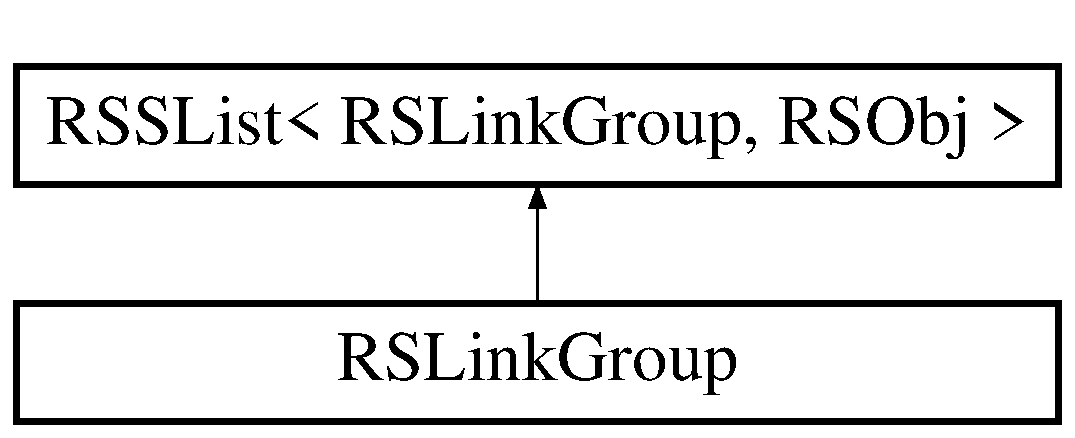
\includegraphics[height=2cm]{classRSLinkGroup}
\end{center}
\end{figure}
\subsection*{Public Member Functions}
\begin{DoxyCompactItemize}
\item 
bool {\bfseries HasA} (RSType type)\label{classRSLinkGroup_a09ff23048e50a78269a5afef1023c805}

\item 
void {\bfseries init} ({\bf RSObj} $\ast$\_\-prt, RSTypeMask tmask)\label{classRSLinkGroup_a3e8eeabe31cc2c627108ae6b063a0974}

\item 
void {\bfseries prepend} ({\bf RSLink} $\ast$lnk)\label{classRSLinkGroup_aa1d93e58ef28b1c8362d2ff7b1b646a0}

\item 
void {\bfseries append} ({\bf RSLink} $\ast$lnk)\label{classRSLinkGroup_ae288366c6b97a2e4324cddb78cdaaa0b}

\item 
void {\bfseries remove} ({\bf RSLink} $\ast$lnk)\label{classRSLinkGroup_a57fcbdedd72e75aa589e64063d2c764a}

\end{DoxyCompactItemize}
\subsection*{Data Fields}
\begin{DoxyCompactItemize}
\item 
{\bf RSLink} $\ast$ {\bfseries cld}\label{classRSLinkGroup_a2687c9fa2cbac82c52e3dfa30d7db47e}

\item 
{\bf RSLink} $\ast$ {\bfseries lcld}\label{classRSLinkGroup_a7ee22bc3581cc2dca827dd0138ea2afe}

\item 
RSTypeMask {\bfseries rs\_\-type\_\-mask}\label{classRSLinkGroup_af9c1848c92c27146984d97ea8a043f19}

\item 
unsigned {\bfseries size}\label{classRSLinkGroup_ad6d4ee713bb4544b5e582cde75fb14d5}

\end{DoxyCompactItemize}


\subsection{Detailed Description}


Definition at line 199 of file RecoUtil.hh.

The documentation for this class was generated from the following files:\begin{DoxyCompactItemize}
\item 
RecoUtil.hh\item 
RecoUtil.cc\end{DoxyCompactItemize}

\section{RSList$<$ \_\-Tp\_\-self, \_\-Tp\_\-prt $>$ Class Template Reference}
\label{classRSList}\index{RSList@{RSList}}
Inheritance diagram for RSList$<$ \_\-Tp\_\-self, \_\-Tp\_\-prt $>$::\begin{figure}[H]
\begin{center}
\leavevmode
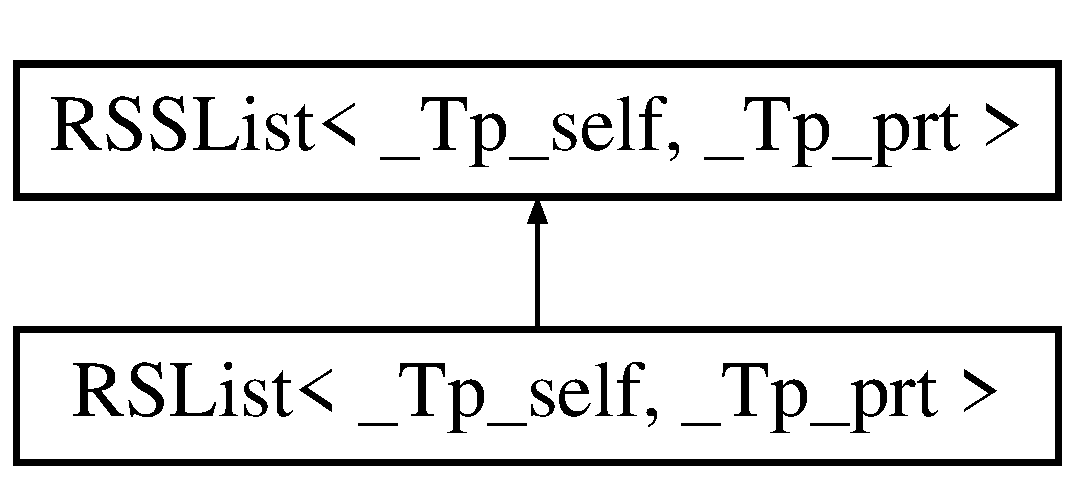
\includegraphics[height=2cm]{classRSList}
\end{center}
\end{figure}
\subsection*{Data Fields}
\begin{DoxyCompactItemize}
\item 
\_\-Tp\_\-self $\ast$ {\bfseries prv}\label{classRSList_acb26209a58ad251d0c451985f6f612dd}

\end{DoxyCompactItemize}


\subsection{Detailed Description}
\subsubsection*{template$<$class \_\-Tp\_\-self, class \_\-Tp\_\-prt$>$ class RSList$<$ \_\-Tp\_\-self, \_\-Tp\_\-prt $>$}



Definition at line 188 of file RecoUtil.hh.

The documentation for this class was generated from the following file:\begin{DoxyCompactItemize}
\item 
RecoUtil.hh\end{DoxyCompactItemize}

\section{RSObj Class Reference}
\label{classRSObj}\index{RSObj@{RSObj}}


Class for ???  


{\ttfamily \#include $<$RecoUtil.hh$>$}Inheritance diagram for RSObj::\begin{figure}[H]
\begin{center}
\leavevmode
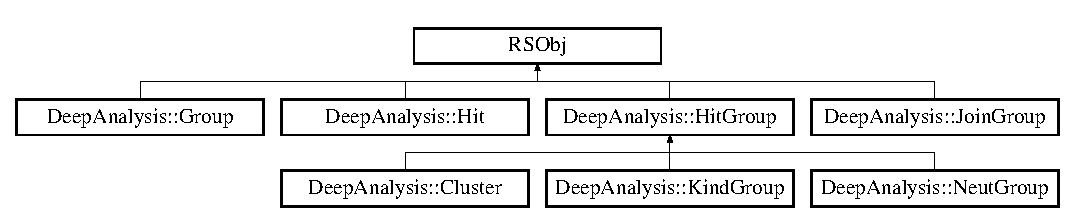
\includegraphics[height=2.54545cm]{classRSObj}
\end{center}
\end{figure}
\subsection*{Public Member Functions}
\begin{DoxyCompactItemize}
\item 
{\footnotesize template$<$class \_\-Tp $>$ }\\bool {\bf IsA} ()\label{classRSObj_af997cbf6eb1ca78a2ae26919322139cd}

\begin{DoxyCompactList}\small\item\em Check if the class is a real \doxyref{RSObj}{p.}{classRSObj}. \item\end{DoxyCompactList}\item 
{\footnotesize template$<$class \_\-Tp $>$ }\\unsigned {\bfseries getNumberOf} ()\label{classRSObj_a7bf3818a093b0fecca70622665f18831}

\item 
{\footnotesize template$<$class \_\-Tp $>$ }\\\_\-Tp $\ast$ {\bfseries getChild} ()\label{classRSObj_a5b3e9f2b277060e6eab66baca7882cbc}

\item 
{\footnotesize template$<$class \_\-Tp $>$ }\\unsigned {\bfseries getNumberOfParents} ()\label{classRSObj_a4b9640e76f27becb8a2cfa3fb1b2c499}

\item 
{\footnotesize template$<$class \_\-Tp $>$ }\\\_\-Tp $\ast$ {\bfseries getParent} ()\label{classRSObj_a84ab8185d507640a6b5cb992de276f27}

\item 
{\bf RSLink} $\ast$ {\bfseries getPrtLink} ({\bf RSObj} $\ast$\_\-prt)\label{classRSObj_af5deb1b2ef4aa69891710ccd2e8ce7ff}

\item 
void {\bfseries remove} ({\bf RSLinkGroup} $\ast$lg)\label{classRSObj_a7b22f5e142588135000e6da11ee010a6}

\item 
unsigned {\bfseries getNumberOf} (RSType type)\label{classRSObj_ab307a0d0940c25a39dd9a1e62c3b8897}

\item 
{\bf RSObj} $\ast$ {\bfseries getParent} (RSType type)\label{classRSObj_a2e987891a30b45701052fd6655df5212}

\item 
bool {\bfseries IsA} (RSType type)\label{classRSObj_a416c4b1b47144ae97331b91bded592ab}

\end{DoxyCompactItemize}
\subsection*{Data Fields}
\begin{DoxyCompactItemize}
\item 
RSTypeMask {\bfseries rs\_\-type\_\-mask}\label{classRSObj_a3ba7c192ba8c0b4f672e107a4ad058ba}

\item 
{\bf RSLinkGroup} $\ast$ {\bfseries cld}\label{classRSObj_ac928b0eb5f69e665a5b5c34ff629e9da}

\item 
{\bf RSLink} $\ast$ {\bfseries prt}\label{classRSObj_a6fea94d99cb0257d1a889110d7ff3f0f}

\end{DoxyCompactItemize}
\subsection*{Protected Member Functions}
\begin{DoxyCompactItemize}
\item 
{\bfseries RSObj} (RSType type)\label{classRSObj_af465287275f7776fdd5f0f8cd6c313f8}

\item 
void {\bfseries AddRSType} (RSType type)\label{classRSObj_a4a343567a829b0ca685bfaa03b37d8b9}

\end{DoxyCompactItemize}


\subsection{Detailed Description}
Class for ??? 

Definition at line 217 of file RecoUtil.hh.

The documentation for this class was generated from the following files:\begin{DoxyCompactItemize}
\item 
RecoUtil.hh\item 
RecoUtil.cc\end{DoxyCompactItemize}

\section{RSParentIterator$<$ \_\-Tp $>$ Class Template Reference}
\label{classRSParentIterator}\index{RSParentIterator@{RSParentIterator}}
Inheritance diagram for RSParentIterator$<$ \_\-Tp $>$::\begin{figure}[H]
\begin{center}
\leavevmode
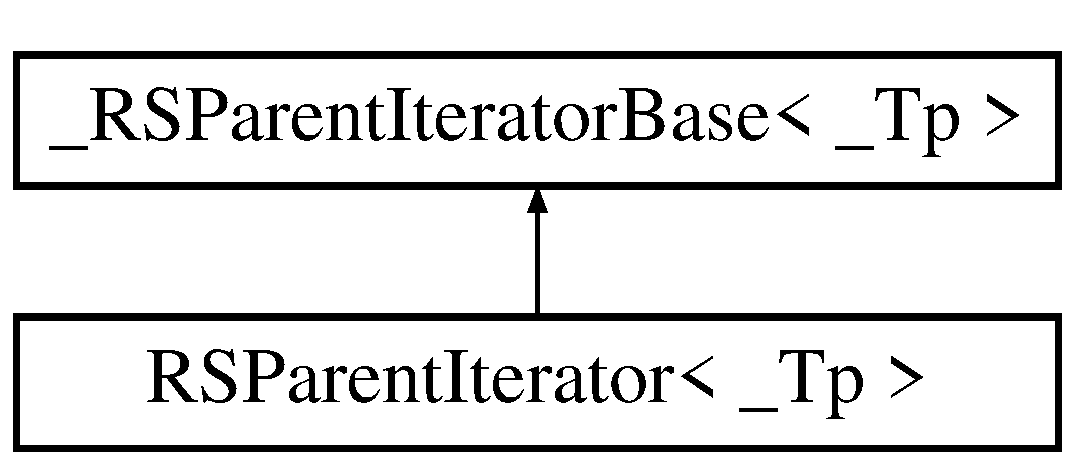
\includegraphics[height=2cm]{classRSParentIterator}
\end{center}
\end{figure}
\subsection*{Public Member Functions}
\begin{DoxyCompactItemize}
\item 
{\bfseries RSParentIterator} ({\bf RSObj} $\ast$\_\-root)\label{classRSParentIterator_a9617420a9952b2226df03c6c3f63875a}

\item 
bool {\bfseries next} ()\label{classRSParentIterator_a6885cd9f51ba64293cf0c4006b956dd7}

\end{DoxyCompactItemize}
\subsection*{Private Member Functions}
\begin{DoxyCompactItemize}
\item 
void {\bfseries \_\-find\_\-first} ()\label{classRSParentIterator_a710e28d238ff48bb73912f506a6601e4}

\item 
void {\bfseries \_\-find\_\-next} ()\label{classRSParentIterator_ad51eac67fa21053e85720cd673970d85}

\end{DoxyCompactItemize}


\subsection{Detailed Description}
\subsubsection*{template$<$class \_\-Tp$>$ class RSParentIterator$<$ \_\-Tp $>$}



Definition at line 514 of file RecoUtil.hh.

The documentation for this class was generated from the following file:\begin{DoxyCompactItemize}
\item 
RecoUtil.hh\end{DoxyCompactItemize}

\section{RSSList$<$ \_\-Tp\_\-self, \_\-Tp\_\-prt $>$ Class Template Reference}
\label{classRSSList}\index{RSSList@{RSSList}}
Inheritance diagram for RSSList$<$ \_\-Tp\_\-self, \_\-Tp\_\-prt $>$::\begin{figure}[H]
\begin{center}
\leavevmode
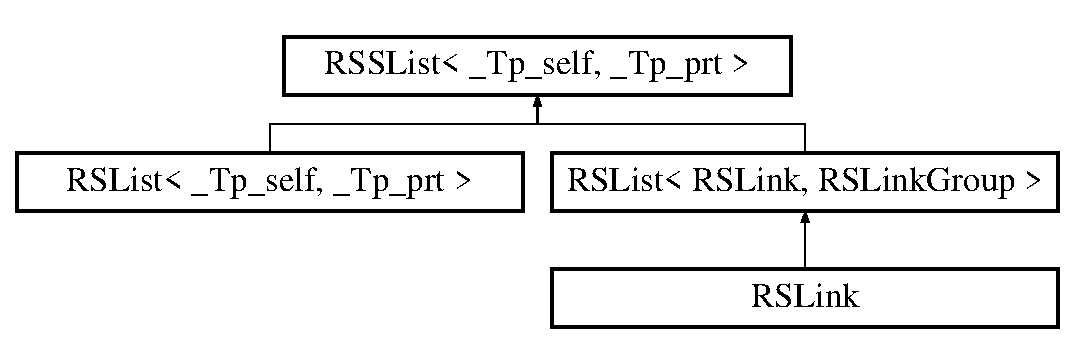
\includegraphics[height=3cm]{classRSSList}
\end{center}
\end{figure}
\subsection*{Data Fields}
\begin{DoxyCompactItemize}
\item 
\_\-Tp\_\-prt $\ast$ {\bfseries prt}\label{classRSSList_a32492faa38b9366095481804cd97bcb4}

\item 
\_\-Tp\_\-self $\ast$ {\bfseries nxt}\label{classRSSList_a871423ffbc31df90605c30c123b2705b}

\end{DoxyCompactItemize}


\subsection{Detailed Description}
\subsubsection*{template$<$class \_\-Tp\_\-self, class \_\-Tp\_\-prt$>$ class RSSList$<$ \_\-Tp\_\-self, \_\-Tp\_\-prt $>$}



Definition at line 181 of file RecoUtil.hh.

The documentation for this class was generated from the following file:\begin{DoxyCompactItemize}
\item 
RecoUtil.hh\end{DoxyCompactItemize}

\section{SpaceHolder$<$ \_\-Tp $>$ Class Template Reference}
\label{classSpaceHolder}\index{SpaceHolder@{SpaceHolder}}


Full version.  


{\ttfamily \#include $<$RecoUtil.hh$>$}Inheritance diagram for SpaceHolder$<$ \_\-Tp $>$::\begin{figure}[H]
\begin{center}
\leavevmode
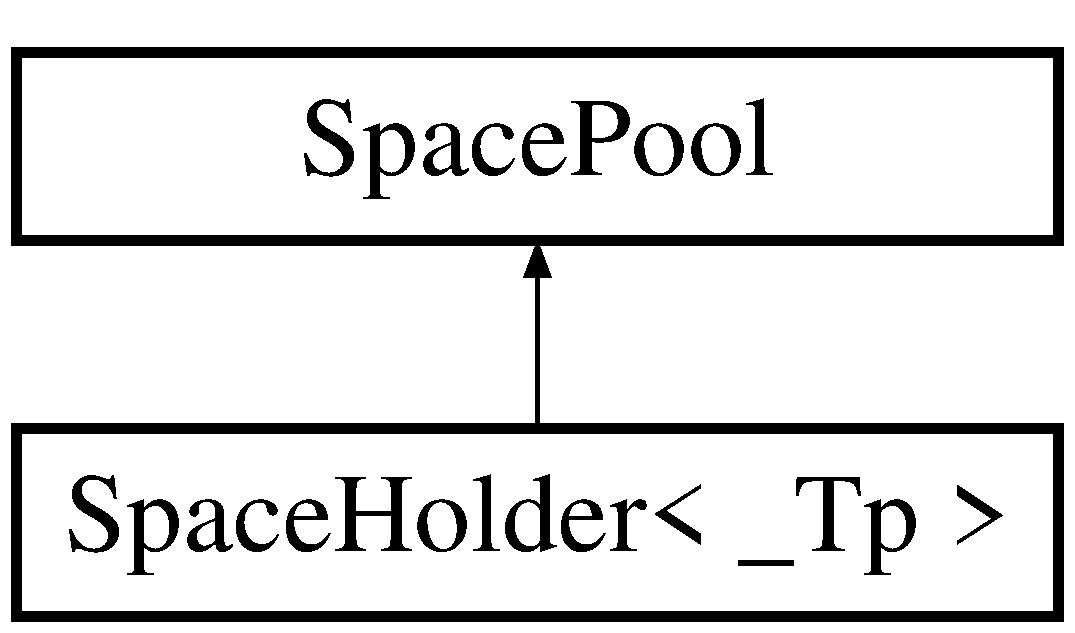
\includegraphics[height=2cm]{classSpaceHolder}
\end{center}
\end{figure}
\subsection*{Public Member Functions}
\begin{DoxyCompactItemize}
\item 
{\bf SpaceHolder} ({\bf SpacePool} \&pool, unsigned prealloc=256)\label{classSpaceHolder_a54fc136f865a5eaacf4d0a69383185dd}

\begin{DoxyCompactList}\small\item\em Constructor. \item\end{DoxyCompactList}\item 
virtual {\bf $\sim$SpaceHolder} ()\label{classSpaceHolder_a93204642d73171e89653999e48e6c277}

\begin{DoxyCompactList}\small\item\em Destructor. \item\end{DoxyCompactList}\item 
\_\-Tp $\ast$ {\bf array} (unsigned n)
\begin{DoxyCompactList}\small\item\em Create array of type \_\-Tp. \item\end{DoxyCompactList}\item 
\_\-Tp $\ast$ {\bf alloc} ()\label{classSpaceHolder_a49d2515207bf9decdf4174851f99e8dd}

\begin{DoxyCompactList}\small\item\em Allocate space for \_\-Tp. \item\end{DoxyCompactList}\end{DoxyCompactItemize}
\subsection*{Private Member Functions}
\begin{DoxyCompactItemize}
\item 
{\bfseries SpaceHolder} ({\bf SpaceHolder}$<$ \_\-Tp $>$ \&x, bool)\label{classSpaceHolder_a81f7ae3364a9449ec8ff81067bf83a53}

\end{DoxyCompactItemize}
\subsection*{Private Attributes}
\begin{DoxyCompactItemize}
\item 
\_\-Tp $\ast$ {\bfseries data}\label{classSpaceHolder_a8ccb66b0e83e4290c6714aa60fda6ace}

\end{DoxyCompactItemize}


\subsection{Detailed Description}
\subsubsection*{template$<$class \_\-Tp$>$ class SpaceHolder$<$ \_\-Tp $>$}

Full version. Items must have ctor and dtor This version can be used with any class, but can be significantly slower then \doxyref{FastSpaceHolder}{p.}{classFastSpaceHolder} 

Definition at line 70 of file RecoUtil.hh.

\subsection{Member Function Documentation}
\index{SpaceHolder@{SpaceHolder}!array@{array}}
\index{array@{array}!SpaceHolder@{SpaceHolder}}
\subsubsection[{array}]{\setlength{\rightskip}{0pt plus 5cm}template$<$class \_\-Tp$>$ \_\-Tp$\ast$ {\bf SpaceHolder}$<$ \_\-Tp $>$::array (unsigned {\em n})\hspace{0.3cm}{\ttfamily  [inline]}}\label{classSpaceHolder_a0baa4414dd62ccef8d783bfa2fe5b479}


Create array of type \_\-Tp. 
\begin{DoxyParams}{Parameters}
\item[{\em n}]number of elements in array ? \end{DoxyParams}


Definition at line 92 of file RecoUtil.hh.

References SpacePool::count.

Referenced by SpaceHolder$<$ \_\-Tp $>$::alloc().

The documentation for this class was generated from the following file:\begin{DoxyCompactItemize}
\item 
RecoUtil.hh\end{DoxyCompactItemize}

\section{SpacePool Class Reference}
\label{classSpacePool}\index{SpacePool@{SpacePool}}


This class is to provide some base class for all templated implementations.  


{\ttfamily \#include $<$RecoUtil.hh$>$}Inheritance diagram for SpacePool::\begin{figure}[H]
\begin{center}
\leavevmode
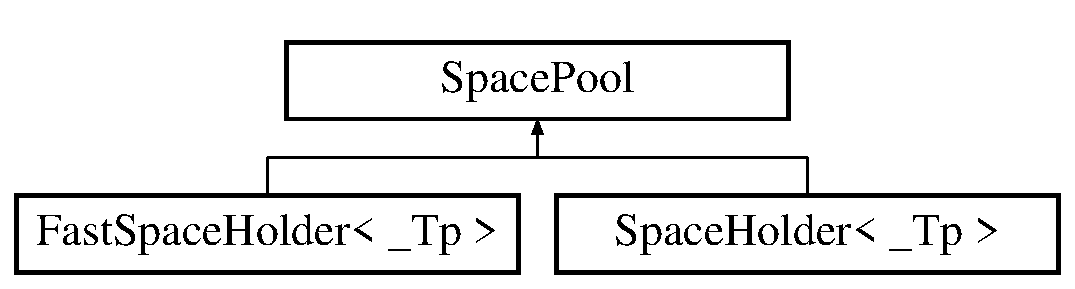
\includegraphics[height=2cm]{classSpacePool}
\end{center}
\end{figure}
\subsection*{Public Member Functions}
\begin{DoxyCompactItemize}
\item 
{\bf SpacePool} (unsigned prealloc=256)\label{classSpacePool_a4778bf95fa19030a2eda2b9652ca66fb}

\begin{DoxyCompactList}\small\item\em Constructor. \item\end{DoxyCompactList}\item 
{\bf SpacePool} ({\bf SpacePool} \&x, unsigned prealloc=256)\label{classSpacePool_ae5816739b4f2ed2b1a41a989e692a644}

\begin{DoxyCompactList}\small\item\em Constructor. \item\end{DoxyCompactList}\item 
virtual {\bf $\sim$SpacePool} ()\label{classSpacePool_a8ddca1507b0d3112b5304572d4a83f97}

\begin{DoxyCompactList}\small\item\em Destructor. \item\end{DoxyCompactList}\end{DoxyCompactItemize}
\subsection*{Protected Member Functions}
\begin{DoxyCompactItemize}
\item 
void {\bfseries connect\_\-to} ({\bf SpacePool} \&x)\label{classSpacePool_a3d1b4392f58b92aed09ac972b1244114}

\item 
{\bfseries SpacePool} ({\bf SpacePool} \&x, bool)\label{classSpacePool_ab80170ef5ee1fbc371ea2ff4ead7a38b}

\end{DoxyCompactItemize}
\subsection*{Protected Attributes}
\begin{DoxyCompactItemize}
\item 
unsigned {\bf count}\label{classSpacePool_ae6b1754e19e2d105a2d3ea870bdca86f}

\begin{DoxyCompactList}\small\item\em common data in all holders \item\end{DoxyCompactList}\item 
unsigned {\bfseries alloced}\label{classSpacePool_a5acf9c577dd6d872d69c24916026f002}

\item 
unsigned {\bfseries \_\-prealloc}\label{classSpacePool_ab88631665439889f3c8981841f6c8ad1}

\end{DoxyCompactItemize}
\subsection*{Private Attributes}
\begin{DoxyCompactItemize}
\item 
{\bf SpacePool} $\ast$ {\bfseries next}\label{classSpacePool_acdbefd16991b86ea2397997074193484}

\end{DoxyCompactItemize}


\subsection{Detailed Description}
This class is to provide some base class for all templated implementations. 

Definition at line 31 of file RecoUtil.hh.

The documentation for this class was generated from the following file:\begin{DoxyCompactItemize}
\item 
RecoUtil.hh\end{DoxyCompactItemize}

\section{DeepAnalysis::SpecialHist2D Class Reference}
\label{classDeepAnalysis_1_1SpecialHist2D}\index{DeepAnalysis::SpecialHist2D@{DeepAnalysis::SpecialHist2D}}


Special 2D histograms.  


{\ttfamily \#include $<$DeepAnalysis.hh$>$}Inheritance diagram for DeepAnalysis::SpecialHist2D::\begin{figure}[H]
\begin{center}
\leavevmode
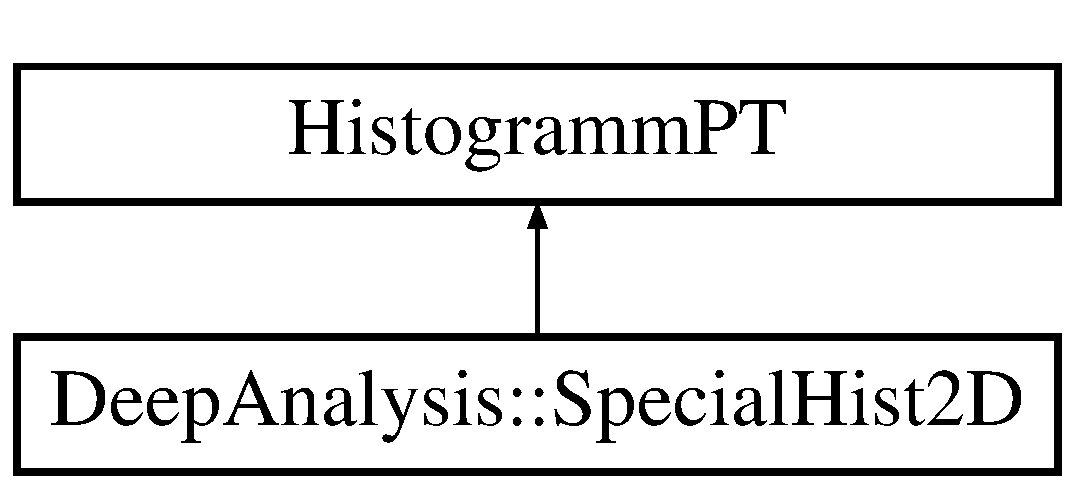
\includegraphics[height=2cm]{classDeepAnalysis_1_1SpecialHist2D}
\end{center}
\end{figure}
\subsection*{Public Member Functions}
\begin{DoxyCompactItemize}
\item 
virtual bool {\bf Book} (const {\bf MinMaxRange}$<$ double $>$ \&p\_\-lim, const {\bf MinMaxRange}$<$ double $>$ \&t\_\-lim, double \_\-step=0.006)\label{classDeepAnalysis_1_1SpecialHist2D_a4e0ed25d3a28a50145c229cac8732836}

\begin{DoxyCompactList}\small\item\em Book histogram. \item\end{DoxyCompactList}\end{DoxyCompactItemize}


\subsection{Detailed Description}
Special 2D histograms. 

Definition at line 836 of file DeepAnalysis.hh.

The documentation for this class was generated from the following file:\begin{DoxyCompactItemize}
\item 
DeepAnalysis.hh\end{DoxyCompactItemize}

\printindex
\end{document}
